%%%%%%%%%%%%%%%%%%%% book.tex %%%%%%%%%%%%%%%%%%%%%%%%%%%%%
%
% sample root file for the chapters of your "monograph"
%
% Use this file as a template for your own input.
%
%%%%%%%%%%%%%%%% Springer-Verlag %%%%%%%%%%%%%%%%%%%%%%%%%%


% RECOMMENDED %%%%%%%%%%%%%%%%%%%%%%%%%%%%%%%%%%%%%%%%%%%%%%%%%%%
\documentclass[graybox,envcountchap,a4paper]{svmono}

% choose options for [] as required from the list
% in the Reference Guide

%\usepackage{mathptmx}
%\usepackage{helvet}
%\usepackage{courier}
%

%% For language-specific hyphenations etc.
\usepackage[english]{babel}
\usepackage[utf8]{inputenc} % Required for inputting international characters
\usepackage[T1]{fontenc} % Output font encoding for international characters
\usepackage{lmodern}
% For subfigures
\usepackage{subcaption}
%\captionsetup{compatibility=false}
%Import the natbib package and sets a bibliography  and citation styles
\usepackage{natbib}
%\setcitestyle{open={[},authoryear,close={]}}
% For nice links
%\usepackage{url}
%Arbitrary size font selection 
\usepackage{type1cm}         
\usepackage{makeidx}         % allows index generation
%\usepackage{cropmark}		% fixes \printindex
\usepackage{graphicx}        % standard LaTeX graphics tool
% when including figure files
\graphicspath{{figures/}}
\usepackage{multicol}        % used for the two-column index
\usepackage[bottom]{footmisc}% places footnotes at page bottom

\usepackage{newtxtext}       % 
\usepackage{newtxmath}       % selects Times Roman as basic font
\usepackage{fancyhdr}% http://ctan.org/pkg/fancyhdr

\usepackage{hyperref}
\hypersetup{
	pdftitle={Mining software development projects},
	pdfauthor={Saimir Bala},
	pdfkeywords={software development, business process management, visualisation, project mining},
	pdfsubject={mining software development projects},
	bookmarksopen=true,
	bookmarksopenlevel=0,
	hypertexnames=true,
	colorlinks=true,       % false: boxed links; true: colored links
%	linkcolor=Firebrick3,          % color of internal links (change box color with linkbordercolor)
%	%linkbordercolor=RedOrange,    
	citecolor=Blue4,        % color of links to bibliography
%	filecolor=magenta,      % color of file links
	urlcolor=blue,           % color of external links
	pdfstartview={FitV},
	unicode=true,
	breaklinks=true,
}

\urlstyle{same}

% For playing with colors in tabular environments
\usepackage{colortbl}

% Compressed, sorted lists of numerical or partly-numerical citations, as regular text or as superscripts
%\usepackage{cite} 

%% For math symbols, such as \nexists
%\usepackage{amssymb}
%% For more math symbols, such as \mapsfrom
%\usepackage{stmaryrd}
\usepackage{textcomp}
%% For advanced graphics
%%% For including figures, graphicx.sty has been loaded in
%%% elsarticle.cls. If you prefer to use the old commands
%%% please give \usepackage{epsfig}
%% For equations, arrays of equations, defining operator names, etc.
%\usepackage{amsmath}
%% For cursive math
%\usepackage{mathrsfs}
%% For math symbols, such as \nexists
%\usepackage{amssymb}
%%% For math environments, such as "definition"
%%\usepackage{amsthm}
%%\theoremstyle{definition}
%%\newdefinition{definition}{Definition}[section]
%%\newtheorem{theorem}{Theorem}[section]
%% For enumerating the line numbers
%\usepackage[left]{lineno}
% For side notes, missing figures and inline to-do's
\usepackage[textsize=scriptsize,backgroundcolor=orange!50]{todonotes}
%% For specifying kewords and acronyms
\usepackage[nonumberlist,acronym]{glossaries}
\glsdisablehyper
%% For commenting out some parts of the text
%\usepackage{comment}
%%\usepackage{etoolbox}
%%\makeatletter
%%\patchcmd\@combinedblfloats{\box\@outputbox}{\unvbox\@outputbox}{}{%
%%	\errmessage{\noexpand\@combinedblfloats could not be patched}%
%%}%
%%\makeatother
%
%% For smart references
\usepackage{cleveref}
\crefname{algocf}{algorithm}{Algorithms}
\crefname{figure}{figure}{figures}
\crefname{table}{table}{tables}
\crefname{missingfigure}{fig.}{figs.}
\crefname{lstlisting}{listing}{listings}
%\Crefname{algocf}{Algorithm}{Algorithms}
%% To have "Figure 3(a)" in place of "Figure 3a" and  "Table 3(a)" in place of "Table 3a"
%\captionsetup[subfigure]{subrefformat=simple,labelformat=simple}
%    \renewcommand\thesubfigure{(\alph{subfigure})}
\captionsetup[subtable]{subrefformat=simple,labelformat=simple}
    \renewcommand\thesubtable{(\alph{subtable})}

% TikZ/Pgf advanced graphics
\usepackage{tkz-base}
\usetikzlibrary{decorations.pathmorphing,trees,arrows,shapes,automata}
%Make a tree diagram
\usepackage{forest}
%% To use inline and other fancy list-like environments (e.g., inparaenum)
%\usepackage{paralist}
%% To divide a text line into multiple columns
%\usepackage{multicol}
%% To create good-looking book-style tables
\usepackage{booktabs}
\usepackage[normalem]{ulem}
\useunder{\uline}{\ul}{}
\usepackage{longtable}
%% To play around with list environments
%\usepackage{enumitem}
% To create multirow cells in tables
\usepackage{multirow}
%% To create rotated cells in tables
%\usepackage{rotating}
%%\usepackage{array}
%% To create enumerated lists, whose numbering is reversed
%\usepackage{etaremune}
%%% To make algorithmic nice-looking pseudocode
\usepackage[linesnumbered,ruled,noline]{algorithm2e}
%%% For creating side-notes
%% \usepackage{marginnote}
%% For superimposing symbols over one another within math env.
%\usepackage{mathtools}
%% For strange math symbols like \Dashv
%\usepackage{mathabx}
%% For LaTeX if/then statements
%\usepackage{ifthen}
%% For strike-through cancellations
%\usepackage[normalem]{ulem}
%%% The lineno packages adds line numbers. Start line numbering with
%%% \begin{linenumbers}, end it with \end{linenumbers}. Or switch it on
%%% for the whole article with \linenumbers.
%\usepackage{lineno}
%% For highlighted text
%\usepackage{soul}
\usepackage{float}
%% To put table environments and co. side by side
%%\usepackage{floatrow}
%%\floatsetup[table]{style=plaintop}
%% To add dummy text
%\usepackage{lipsum}
%% To have newlines in cells, with commands such as \makecell or \thead
%\usepackage{makecell}
%% To enable text protrusion
\usepackage{microtype}
%%\usepackage[showframe]{geometry}
\usepackage{xspace}
\usepackage{pifont}
\newcommand{\cmark}{\ding{51}}%
\newcommand{\xmark}{\ding{55}}%
%% For code
\usepackage{listings}

%
%\AtBeginDocument{
%	\hypersetup{pdftitle=Mining software development projects} % Set the PDF's title to your title
%	\hypersetup{pdfauthor=Saimir Bala} % Set the PDF's author to your name
%	\hypersetup{pdfkeywords={software development, business process management, visualisation, project mining}} % Set the PDF's keywords to your keywords
%}


% see the list of further useful packages
% in the Reference Guide

\makeindex             % used for the subject index
                       % please use the style svind.ist with
                       % your makeindex program

%%%%%%%%%%%%%%%%%%%%%%%%%%%%%%%%%%%%%%%%%%%%%%%%%%%%%%%%%%%%%%%%%%%%%

\begin{document}

\author{Saimir Bala}
\title{Mining software development projects}
\subtitle{-- Monograph --}
%\maketitle

\frontmatter%%%%%%%%%%%%%%%%%%%%%%%%%%%%%%%%%%%%%%%%%%%%%%%%%%%%%%


%%%%%%%%%%%%%%%%%%%%%%% dedic.tex %%%%%%%%%%%%%%%%%%%%%%%%%%%%%%%%%
%
% sample dedication
%
% Use this file as a template for your own input.
%
%%%%%%%%%%%%%%%%%%%%%%%% Springer %%%%%%%%%%%%%%%%%%%%%%%%%%

\begin{dedication}
To my family 
– Saimir
\end{dedication}






\Extrachap{Abstract}

Software development is a highly flexible endeavor. Yet, software development projects
have specific requirements about quality, costs and time to deliver. Therefore, there is need
for monitoring and controlling the software development process. This problem is tackled
separately by three different disciplines, but existing approaches still fail at delivering process
knowledge about software development that can be easily understood by managers. This
dissertation develops novel methods and algorithms that can be used to extract process
knowledge from software development trace data. As a result, it can be positioned as a
bridge between the process mining discipline and the area of software engineering. From
a research point of view, the outcomes of this dissertation are a building block to further
cross-fertilize research streams on process mining and software engineering. From a practical
point of view, the outcomes of this dissertation allow the project manager to obtain a more
familiar means of analysis on software development such as a process view.

\todo[inline]{KR: Confusing. It is not possible to understand the problem and your solution is also not clear. 
	
	You start with software development and then process appears. Later you bring process mining, but it is not clear why. Also, you talk about trace out of the blue. Maybe you can start from process of software developmentt}


%\include{chap/foreword}
%\include{chap/preface}
%%%%%%%%%%%%%%%%%%%%%%acknow.tex%%%%%%%%%%%%%%%%%%%%%%%%%%%%%%%%%%%%%%%%%
% sample acknowledgement chapter
%
% Use this file as a template for your own input.
%
%%%%%%%%%%%%%%%%%%%%%%%% Springer %%%%%%%%%%%%%%%%%%%%%%%%%%

\extrachap{Acknowledgements}

Thanks to Jan and the other people without whom I would not be here. The list is quite long.



\tableofcontents

\listoffigures

\listoftables

%%%%%%%%%%%%%%%%%%%%%%acronym.tex%%%%%%%%%%%%%%%%%%%%%%%%%%%%%%%%%%%%%%%%%
% sample list of acronyms
%
% Use this file as a template for your own input.
%
%%%%%%%%%%%%%%%%%%%%%%%% Springer %%%%%%%%%%%%%%%%%%%%%%%%%%

\extrachap{Acronyms}

List of abbreviations used in this thesis.

\begin{description}[CABR]
\item[BPM]{Business Process Management}
\item[XES]{eXtensible Event Stream}
%\item[CABR]{Spelled-out abbreviation and definition}
\end{description}

\mainmatter%%%%%%%%%%%%%%%%%%%%%%%%%%%%%%%%%%%%%%%%%%%%%%%%%%%%%%%
%\include{part}

%\include{chap/chapter}

\chapter{Introduction}
\label{introduction} % Always give a unique label
% use \chaptermark{}
% to alter or adjust the chapter heading in the running head

\abstract*{This chapter provides an introduction of this doctoral thesis. \Cref{sec:1} provides the motivation
\Cref{sec:2} background ... 
\Cref{sec:3} Research paradigm -- Peffers
\Cref{sec:4} ... Structure
}

\abstract{This chapter provides an introduction of this doctoral thesis. \Cref{sec:1} provides the motivation
	\Cref{sec:2} background ... 
	\Cref{sec:3} Research paradigm -- Peffers
	\Cref{sec:4} Provides ... Structure}



\chapter{Problem Background}
\label{ch2:problem-background}

\section{Software Process}
\label{sec:ch2-software-process}

\section{Theorizing the Software Process}
\label{sec:ch2-theorizing}

\subsection{Organization Routines}
\label{subsec:org-stud}

\subsection{Coordination Theory}

\subsection{Business Process Management}

\subsection{Language-Action (Perspective)}

Winograd \& Flores~\cite{Winograd1986a}

\section{Tool Support for Software Development Processes}
\label{sec:ch2-tool-support}

\section{Software Process Monitoring }
\label{sec:ch2-sw-p-monitoring}

\subsection{What is important to be monitored}

\subsection{How far it is difficult}

\section{Research Questions}
\label{sec:ch2-research-questions}

Addressed in the main chapters.

\begin{description}
	\item[RQ1] description
	\item[RQ2] description
	\item[RQ3] description
\end{description}


\section{Software Process}
\label{sec:ch2-software-process}


\chapter{Solution Background}
\label{chap:ch3-solution-background}

\section{Process Mining}
\label{sec:process-mining}

\section{Mining Software Repositories}
\label{sec:msr}

\section{Software Visualization}
\label{sec:visualization}

\section{Text Mining}
\label{sec:text-mining}

\section{Relevant Techniques}
\label{sec:relevant-techniques}

Here go the techniques relevant for this thesis.



\chapter{Mining Project-Oriented Business Processes}

\todo[inline]{Here goes BPM1}

The class of processes that we discuss in this chapter are long-term engineering
projects. These processes have specific requirements for monitoring. First, they
are executed only once according to the specific needs of a particular project, and
only partially according to recurring process descriptions. Second, they involve
various actors that typically document their work in a semi-structured way using
text and tables. Third, work in the project is usually subject to constraints
regarding the start and end and the temporal order. Fourth, there is typically
no process engine controlling the execution. Fifth, even though these limitations
in terms of traceability exist, there are usually strong requirements in terms of
tracking when which work was conducted.


Here goes the contribution from BPM1. 

\section{Project-Oriented Business Processes}
\todo[inline]{Rephrase here}

A project-oriented business process can be
defined as an ad-hoc plan that specifies the tasks to be performed within a limited
period of time and with a limited set of resources for achieving a specific goal.
Unlike repetitive business processes for which notations such as BPMN [12] or
EPC [1] are commonly used, project-oriented business processes may be properly
represented with PERT or GANTT models.

\section{Approaches to Mine Project-Oriented Business Processes}
\todo[inline]{Rephrase here}

The problem described has been addressed in the literature from different per-
spectives. The first category of related work tackles the problem by transforming
it into a process mining problem. Consequently, approaches have been developed
to preprocess VCS data such that process mining techniques can be applied, and
hence, a business process can be derived from the log data. In this group, Kindler
et al. [9,10] developed an algorithm for extracting software processes that are
mapped to Petri Nets. Activities, which are not explicit in the logs, are discovered
from their input and output artifacts. However, strong assumptions are made on
the filenames as well as on the software process lifecycle. Rubin et al. in [15] ad-
dressed the problem of engineering processes that are not well documented and
are usually unstructured. They provided a bridge from Kindler et al.’s approach
to ProM [5] in order to mine different process perspectives, such as performance
social network analyses. Rubin et al. [16] applied process mining to the touristicMining Project-Oriented Business Processes
5
industry and obtained user processes from web client logs pursuing the goal of
improving the software system by analyzing the underlying process. Poncin et
al. [14] developed the FRASR framework for preprocessing software repositories
to transform the VCS data to logs that conform to the process mining event log
meta model [4] as utilized in ProM [5]. However, these approaches disregard the
single-instance nature of project-oriented business processes and treat them as
procedures that can be repeated over time.
The second category of related work focuses on the visualization of VCS data
for different purposes. Several approaches study the interaction among develop-
ers over time from a visualization point of view. For instance, Ogawa and Ma
[11] drew storyline pathways to show the story of each developer’s contribution.
Other approaches analyze and visualize VCS data at file level in order to discover
file version evolution. Voinea and Telea [20] introduced an interactive navigation
method to surf file version evolution as well as two methods to cluster versions
of the same file in an abstraction layer. Wu et al. [22] also visualized the evolu-
tions of entire projects at file level, emphasizing the evolution moments. Finally,
several approaches study change prediction with the aim of discovering predic-
tion patterns that can help in the process of software development [24,23]. The
approaches mentioned in this category as well as others that apply similar tech-
niques [6,8,3] focus on studying software evolution from different standpoints.
However, the goal pursued differs in all cases from our goal in that they are not
interested in discovering projects tasks out of the log data, and hence, they lack
an explicit notion of work structure that we need to consider for our purpose.
Our approach combines ideas from both areas, as we aim at identifying tasks
like in the approaches that rely on process mining, but we must cluster the data
in an appropriate way, for which techniques developed in the approaches that
pursue visualization may be adapted or extended.

%\chapter{Uncovering the Hidden Co-Evolution in the Work History of Software Projects}
\chapter{Article 2: Uncovering the Hidden Co-Evolution in the Work History of Software Projects}

{\bfseries \Large Authors:}

\noindent Saimir Bala, Kate Revoredo, 
Jo\~{a}o Carlos de A. R. Gon\c{c}alves,
Fernanda Bai\~{a}o,
Jan Mendling, and Flavia~Santoro \hfill

\bigskip

{\noindent\bfseries \Large Published in: \medskip}

\noindent Business Process Management - 15th International Conference, {BPM}
2017, Barcelona, Spain, September 10-15, 2017, Proceedings

\bigskip

{\noindent\bfseries \Large Abstract: \medskip}


\noindent The monitoring of project-oriented business processes is difficult because their state is fragmented and represented by the progress of different documents and artifacts being worked on. This observation holds in particular for software development projects in which various developers work on different parts of the software concurrently. Prior contributions in this area have proposed a plethora of techniques to analyse and visualize the current state of the software artifact as a product. It is surprising that these techniques are missing to provide insights into what types of work are conducted at different stages of the project and how they are dependent upon another. In this paper, we address this research gap and present a technique for mining the software process including dependencies between artifacts. Our evaluation of various open-source projects demonstrates the applicability of our technique. 


\pagebreak



%\todo[inline]{Link this solution to the existing problem. Say e.g. that the previous solution still lacks information about dependency. We would like to know what is inside a specific square in the BPM1 solution. As well, why some squares are connected.}


%\abstract*{The monitoring of project-oriented business processes is difficult because their state is fragmented and represented by the progress
%	of different documents and artifacts being worked on. This observation
%	holds in particular for software development projects in which various
%	developers work on different parts of the software concurrently. Prior contributions in this area have proposed a plethora of techniques to analyze
%	and visualize the current state of the software artifact as a product. It is
%	surprising that these techniques are missing to provide insights into what
%	types of work are conducted at different stages of the project and how
%	they are dependent upon another. In this paper, we address this research
%	gap and present a technique for mining the software process including
%	dependencies between artifacts. Our evaluation of various open-source
%	projects demonstrates the applicability of our technique.}
%
%The monitoring of project-oriented business processes is difficult because their state is fragmented and represented by the progress
%	of different documents and artifacts being worked on. This observation
%	holds in particular for software development projects in which various
%	developers work on different parts of the software concurrently. Prior contributions in this area have proposed a plethora of techniques to analyze
%	and visualize the current state of the software artifact as a product. It is
%	surprising that these techniques are missing to provide insights into what
%	types of work are conducted at different stages of the project and how
%	they are dependent upon another. In this paper, we address this research
%	gap and present a technique for mining the software process including
%	dependencies between artifacts. Our evaluation of various open-source
%	projects demonstrates the applicability of our technique.
%	
%	
%	In this section, we focus on a specific class of project-oriented business processes,
%	namely software development processes. These processes share some common
%	characteristics. First, they involve various resources with different roles. In the 
%	simplest case, we can distinguish project managers and project participants.
%	Project managers are responsible for managing the development process and
%	supervising the work of the project participants, who in turn are responsible for
%	specific work tasks. Second, such processes are usually subject to constraints in
%	terms of cost, time and quality, which is mostly associated with the performance
%	of each of the work tasks. Third, the project participants work on a plethora of
%	artifacts, which are logically organized in a hierarchical structure, with complex
%	interdependencies among them. Given these characteristics, it is the goal of the project manager to organize the software development process in such a way
%	that the work on different files and tasks reflects the complex interdependencies,
%	the constraints and the available participants. Therefore, it is important for the
%	manager to understand the work history of the process in order to monitor the
%	progress systematically.
%
%
%This chapter is structured as follows. Section~\ref{sec:bpm2017background} describes the research problem along with its requirements and summarizes insights from prior research. Section~\ref{sec:bpm2017approach} presents our approach in detail. Section~\ref{sec:bpm2017evaluation} shows a prototypical implementation and evaluates its applicability both in a use case scenario and on real world projects from GitHub. Section~\ref{sec:bpm2017conclusion} concludes the paper.
%
%\section{The Problem of Case Perspective Discovery}
%
%The case perspective of a process focuses on properties of cases \citep{DBLP:books/sp/Aalst16}. There are several characteristics of the cases that are relevant for monitoring. For example in an purchase-to-pay process, along with the information about the order of activities executed to handle an order, it may also be relevant to observe which customer originated the order, the number of products order, the people who handled the order and what data objects were created and maintained to handle the case. In this thesis, extracting information about the characteristics of cases is referred to as \emph{case perspective discovery}.
%
%The problem of case perspective discovery in software development projects aims at uncovering hidden-work dependencies that may exist. They can be structural (e.g., a parent-child relationships between directory and file), functional (e.g., when a method calls an existing library function), or logical. Logical dependencies are complex. One type of such dependencies is when the status of two artifacts evolves similarly through time. These kind of dependencies are not explicit in the structure of the artifact as they are related to the overarching process. Yet, the discovery of such dependencies si vital in order to understand deviations in both planning and maintenance.  
%
%A starting point to detect the hidden work-dependencies is to study the evolution of the various artifacts that are produced. Such evolution is tracked in the history of the various files and other information that is recorded during development. One fundamental system that is used to keep track of the various changes of files is \gls{vcs}. Data from this system can be extracted as a semi-structured dataset. 
%
%%Software tools like \glspl{vcs} do not provide direct support for monitoring work histories.
%%A starting point for analyzing software projects is represented by events that are stored in \glspl{vcs}, which help keeping track of successive versions of artifacts.
%%Table \ref{tab:vcs-log-data} shows an excerpt of log data, where the columns, from left to right, indicate the commit identifier, the project participant who committed the changes, the commit date, the comment written by the project participant and the files affected and the change performed\footnote{cf. unified diff format  \url{https://git-scm.com/docs/git-diff}}. 
%In order to understand the work history and dependencies based upon such data, we identify three major requirements:
%
%\begin{description}
%	\item [\bfseries R1 (Extract the work history):] Discover the process of how artifacts evolve in the project as a \emph{labeled} set of steps. This requirement is difficult because the version changes of a commit in relation to a single file do not directly reveal which type of work has been done. Both commit messages and edit characteristics might inform the labeling.	
%	\item [\bfseries R2 (Uncover Work-Related Dependencies):] Identify that certain work in one part of the project is connected with work in another part. This requirement is difficult because such dependencies might not only exist between files that reside in the same directory. For example, a change in a source code file might have the side effect of triggering work on a configuration file. We refer to this as \emph{co-evolution} of these files.
%	\item [\bfseries R3 (Measure Dependencies):] Determine how strong the co-evolution of different artifacts is. This requirement is difficult because measures of \emph{strength} of dependencies and on the \emph{distance} of   dependent artifacts have to be devised.
%\end{description}


%\section{Related Work }
\label{sec:bpm2017background}
This thesis follows the \gls{dsr} paradigm~\cite{Peffers2008}. In this section, we describe the research problem in more detail and define requirements for a solution. Against these requirements, we analyze related work.
%and some background knowledge important for the understanding of our proposal.

%\subsection{Problem Description}
\label{subsec:prob-desc}
In this work, we focus on a specific class of project-oriented business processes, namely software development processes. These processes share some common characteristics. First, they involve various resources with different roles. In the simplest case, we can distinguish \emph{project managers} and \emph{project participants}. Project managers are responsible for managing the development process and supervising the work of the project participants, who in turn are responsible for specific work tasks. Second, such processes are usually subject to constraints in terms of cost, time and quality, which is mostly associated with the performance of each of the work tasks. Third, the project participants work on a plethora of artifacts, which are logically organized in a hierarchical structure, with complex interdependencies among them.
Given these characteristics, it is the goal of the project manager to organize the software development process in such a way that the work on different files and tasks reflects the complex interdependencies, the constraints and the available participants. Therefore, it is important for the manager to understand the \emph{work history} of the process in order to monitor the progress systematically.

%project specifies the tasks to be performed considering a hierarchy of files, within a limited period of time, and with a limited set of project participants, for achieving a specific goal, typically the release of a new version of a software. Best practices are often used to properly organize the work according, for instance, to good modularization principles. However, monitoring whether this or other guidelines are followed in the actual development process is not easy, due to the lack of an overarching process that defines the work.

%Project managers are interested in an understanding of the running project from a macro level. Useful information is concerns:
%\begin{inparaenum}[\itshape i)]
%	\item project structure;
%	\item profiles of users;
%	\item and the work history.
%\end{inparaenum} Existing tools in software development can help project managers to monitor and control these perspectives individually. For instance, CVS

%Nevertheless, these tools lack on information considering the work process reflected in the artifacts, i.e. artifact evolution, and a dependency among them beyond the structural provided by the hierarchy. Moreover, it is common to have hundreds of versions of thousands of files in a single project, which makes it impractical to browse this data manually.

\input{bpm2017/tables/vcs-data2}

Software tools like \glspl{vcs} do not provide direct support for monitoring work histories, but they provide a good starting point by continuously collecting event data on successive versions of artifacts.
%A starting point for analyzing software projects is represented by events that are stored in \glspl{vcs}, which help keeping track of successive versions of artifacts.
Table \ref{tab:vcs-log-data} shows an excerpt of log data, where the columns, from left to right, indicate the commit identifier, the project participant who committed the changes, the commit date, the comment written by the project participant and the files affected and the change performed\footnote{cf. unified diff format  \url{https://git-scm.com/docs/git-diff}}. In order to understand the work history and dependencies based upon such data, we identify three major requirements:

\begin{description}
	\item [R1 (Extract the work history):] Discover the process of how artifacts evolve in the project as a \emph{labeled} set of steps. This requirement is difficult because the version changes of a commit in relation to a single file do not directly reveal which type of work has been done. Both commit messages and edit characteristics might inform the labeling.	
	\item [R2 (Uncover Work-Related Dependencies):] Identify that certain work in one part of the project is connected with work in another part. This requirement is difficult because such dependencies might not only exist between files that reside in the same directory. For example, a change in a source code file might have the side effect of triggering work on a configuration file. We refer to this as \emph{co-evolution} of these files.
	\item [R3 (Measure Dependencies):] Determine how strong the co-evolution of different artifacts is. This requirement is difficult because measures of \emph{strength} of dependencies and on the \emph{distance} of   dependent artifacts have to be devised.
\end{description}


\subsection{Related Work}
\label{subsec:related}
A solution addressing these requirements can partially build upon research in three main areas:
\begin{inparaenum}[\itshape i)]
	\item work on \gls{msr};
	\item \gls{pm};
	\item and software visualization.
\end{inparaenum}

\input{bpm2017/tables/related-work-table}

Table~\ref{table:related-work} shows that these streams of research have mutual strengths, but no contribution covers the full spectrum. In general, methods from \gls{msr} have a strength in analyzing dependencies in the structure of the software artifact, but an explicit consideration of the type of work is missing. Contributions in this area focus on the users and the artifacts, mining co-evolution or co-change of project parts~\cite{zaidman2008mining,DAmbros2009} and network analysis of file dependency graph based on commit distance~\cite{Zimmermann2008,Abate2009,Weicheng2013}. Hidden work dependencies are mentioned as \emph{logical dependencies}~\cite{Oliva2011}. Also techniques for trend analysis~\cite{Ruohonen2015} and inter-dependencies between developers~\cite{lindberg2016coordinating} are proposed. However, none of these works considers the type of work being done in the process.

In the area of \gls{pm}, research gives more emphasis to the different tasks of the process. Some works focus on applying process mining for software repositories~\cite{Poncin2011a,Mittal2014,Bala2015}. In this context, approaches have been defined that use various queries to extract artifact evolution and resources~\cite{Beheshti2016,Beheshti2013}. There is research on identifying the tasks of the process by elicitation from unstructured data of user comments~\cite{Goncalves2011}. There are also process mining applications that focus on repetitive steps in software engineering, but not on singular project-oriented processes, such as \cite{Kindler2006}. All these works only consider the dependencies between work tasks to a limited extend.

%, but they lack a concept of work dependency. On the other hand, \gls{pm} contributions can help understand the work reflected by the artifacts, although to the best of our knowledge, a solution for hidden artifact dependencies is not existing yet. Moreover, \gls{pm} techniques are limited to recurrent work patterns (e.g., the process of bug fixing) and do not generally apply to the whole software project.

%In the area of \gls{msr}, many works analyze collaborative software development by mining \gls{vcs} log data.

There is also work in the area of software visualization. 
Visualization tools have been proposed in order to allow project managers to have a detailed overview of the software artifact being developed. These tools help to visually inspect artifacts similarities on different levels of granularity~\cite{Voinea2006b}, observe artifacts evolution or project members contribution~\cite{Ripley2007,Greene2015}. In general, they can be characterized as artifact-centric, and largely agnostic to the type of work being done.

%\Cref{table:related-work} summarizes how literature addresses the defined requirements. In general, methods from \gls{msr} are robust on analyzing dependencies in projects, but they lack a concept of work dependency. On the other hand, \gls{pm} contributions can help understand the work reflected by the artifacts, although to the best of our knowledge, a solution for hidden artifact dependencies is not existing yet. Moreover, \gls{pm} techniques are limited to recurrent work patterns (e.g., the process of bug fixing) and do not generally apply to the whole software project.

In the following, we develop a technique that addresses the three requirements and informs prior research on how to extract work histories and to identify the co-evolution of certain parts of a project-oriented software process.



%In this Section, we present closely related work to the approach proposed in this paper. We characterize closely related work as formal studies on providing method to extract or representing software development process. 
%
%Salameh et al. \cite{10.1109/CSIT.2016.7549475}  made a systematic review of literature to discuss Software Visualization and Evolution (SVE) tools and techniques. They analyzed 29 out of 55 papers. They concluded that the main source of information used by such tools is information extracted from software repositories. SVE tools can be classified into five different groups: graph-based, notation-based, matrix-based, metaphor-based and others. Graph-based are the most popular while notation-based are the least. SVEs focus can be either Artifact-centric visualization, Metric-centric visualization, Feature-centric visualization, or Architecture-centric visualization. The authors also identified generic functional requirements for software visualization tools: (i) views \cite{bani2016software}: show different representations; (ii) details-on demand: show more information/details; (iii) filter and search: show something conditionally; (iv) select: mark something as point of interest; (v) re-arrangement: show different arrangements of the data sets (e.g. sort, cluster, and aggregate); (vi) comparison: show the differences between different data sets.
%
%
%In \cite{Mittal:2014:PMS:2591062.2591152}, data achieved from four sources was evaluated: team wiki (used during requirement engineering), version control system (development and maintenance), issue tracking system (corrective and adaptive maintenance) and data generated as a result of constructing software by student teams in an educational setting. The main goal of the paper was to provide metrics and visualizations that better describe the work developed by the students in the discipline. From this analysis, it was possible to observe task distribution among the students in a project or commits behavior. 
%
%% Elsen \cite{DBLP:conf/vissoft/Elsen13} presents the prototype VisGi and a set of strategies for mining and displaying Git repositories. VisGi intends to abstract and visualize the branch structure of a Git, as well as its folder trees. By interpreting branches as groups of aggregated commits, their dependencies are condensed into a directed acyclic graph, and displayed using graph layout strategies. Tagging mechanisms are used to aggregate commits into compact nodes of a group graph. Sunburst diagrams are also proposed to display the content of the branches, the differences between each two branches, and the evolution of a particular selected path. Since the extraction is limited to the last commit of each group, it creates holes in older sections of most repositories. 
%
%%Greene and Fisher \cite{DBLP:conf/vissoft/Greene015} describe ConceptCloud, an interactive browser for SVN and Git repositories which combines an intuitive tag cloud visualization with an underlying concept lattice providing a formal structure for navigation. The authors claim that this solution can be used to answer questions such as \emph{What has happened in this project while I was away/?}, \emph{Which developers collaborate/?}, or \emph{What are the co-changed methods/?}. 
%
%In \cite{DBLP:conf/msr/RayNBNZ15}, Ray et al worry about improving risk analysis, recommendation and program repair techniques by automatic detecting unique changes in a software project history. They argue that unique changes require more expertise or represent code that is more complex or prone to mistakes than the more common similar (or non-unique) changes. Their contribution provides a valuable amount of information to support managers on the monitoring and managing software development processes; %however, they do not focus on visualization issues.
%
%Lehtonen et al.~\cite{DBLP:conf/ejc/LehtonenAKM16} proposed a visualization tool for collecting insights based on data collected through a tracking tool. The authors argue that analysis of this data helped the managers to understand the process more deeply showing what kind of spring lenghts and common deployment times actually exist and the identification of uncommonly long delivery times for some features. %Although the paper is related to ours in the sense that a visualization is proposed to help managers in a better decision making, in our work we focus on explicitin how the work is performed and how dependencies between artifacts combined with containments information can help understand how the development of the software can be improved.
%
%In \cite{Bala2015} a mining approach to help generate GANTT charts was proposed. They allow project managers to visualize work history from the perspective of activities performed inside a workpackage and the resource allocated to the activity.  Data from VCS logs are used for the mining and visualization. 
%
%Based on the literature proposals analyzed, we observed that solutions that deal with monitoring and managing software development process propose visualization tools that use data available from software repositories, version control systems, and IDEs [7]. Many tools have been proposed in order to support managers on the evolution of the software; They have similarities to ours, since it aims to provide insights about the project development to managers, however, they do not consider the files perspective. They do not analyses the evolution of each file over time and their relation, crossing information with structural information, like containments. Moreover, we also contribute presenting a story mining approach for automatically extracting the file evolution and provide representations of the knowledge extracted, thus facilitating the analysis of the managers, and crossing the gathered information.

%\subsection{Story Mining}
\label{subsec:story-mining}

%What is story mining and how we use it in our work
Gon\c{c}alves et al.~\cite{Goncalves2011} proposed a story mining approach to extract process elements from stories, i.e. text descriptions written collaboratively by the process participants. A story is a natural way to transmit and share knowledge. Using both natural language (text) and contextual elements (categorization of parts of the story), storytellers can express their experience and viewpoints about the work processes they participate, interact with and/or perceive. Stories have the advantage of reproducing the situations associated with their contexts - the knowledge that is difficult to capture in interviews or mining from Information Systems logs. Since collectively told, a story incorporates a range of perspectives. Business processes instances can also be viewed as stories played by individuals who perform specific roles depending on the circumstances.

Story Mining  \cite{Goncalves2011} receives as input a story freely written by the participants, describing their work in a particular business process. As an output, the \emph{actors} and the process \emph{activities} executed by them are extracted. To illustrate the approach consider the following story. The terms highlighted in {\bf bold} are the actors of the processes and the terms highlighted in {\color{gray} gray} the activities. 

\begin{figure}[!h]
{ \bf The system} {\color{gray} generates an estimating template consisting of the phases, activities and tasks} selected
for the project or project phase. When planning complete projects the estimating is typically done at the activity level, using the
list of tasks in the work breakdown as input to the estimating process. However {\bf estimators} will likely {\color{gray}add an itemized list of system functions and other deliverables}, to facilitate estimating the construction phase. {\bf Multiple estimators} {\color{gray} prepare estimates for each component}, {\color{gray}compare their estimates}, and {\color{gray}arrive at a final estimate} for each item.
  \label{RB}
\end{figure}

A further step that we developed in our approach is the identification of the relationship between the activities, therefore defining the flow.

%\section{Approach to Discover the Case Perspective}
\label{sec:bpm2017approach}

%In this section, we describe our approach for mining software development projects. First, we give an overview of the approach itself, then we formally define concepts required by our technique.

%Version control systems (VCSs) are used in projects to ensure reliable collaboration.
%We build our technique on \gls{vcs}. In this context, project participants work on files (e.g., text, source code, spread sheets) and commit their changes to a central repository, which maintains information on the work history.

We propose a technique to extract and represent the work history and the dependencies among artifacts of a project-oriented business process. The technique takes as input a \gls{vcs} log and produces analysis data that describe the evolution of the artifacts, along with metrics about their distance and their similarity in terms of work.
The process is depicted in \Cref{fig:visualization-process} and consists of three successive steps towards extracting hidden work dependencies from \gls{vcs} event data. The method works under three main assumptions. First, we assume a \emph{meaningful tree structure}, i.e. the project participants organize the files in a representative hierarchy (e.g., spatially separating documentation from testing into different folders). Second, project participants perform \emph{regular commits} in the \gls{vcs}. Third, project participants write \emph{descriptive comments} that allow other members to understand the changes.

%\begin{itemize}
%	\item [A1:] {\bf Meaningful file tree structure.} The file tree structure in a project represents the structure of work of the project participants.
%	\item [A2:] {\bf Frequent commits.} Commits to the VCS are regularly performed.
%	\item [A3:] {\bf Meaningful comments.} The comments included by project participant when committing their work represent the changes done to the file being commit.
%\end{itemize}
%\vspace*{-.5cm}
\begin{figure}[h]
	\centering
	\includegraphics[width=.9\textwidth]{bpm2017/figures/visualization-process-crop}
	\caption[Approach for generating analysis data from VCS logs]{Approach for generating analysis data from VCS logs}
	\label{fig:visualization-process}
\end{figure}

The first step of the technique is the preprocessing of the \gls{vcs} log received as input. The main goal of this phase is to generate a set of events and store them into a database. Second, we obtain different views on the stored events. In particular, we are interested in observing
\begin{inparaenum}[\itshape i)]
	\item all the commits that affected the files over time;
	\item the amount of change brought by the commits to the files; and
	\item the users who issued such commits.
\end{inparaenum}
The third phase is responsible for considering the different perspectives defined by the project manager and through the generated views extract the necessary knowledge. In the following, we detail the formal concepts and the algorithm of our technique.



%We propose a techniques to extract and represent the work history and the dependencies among artifacts. The process is depicted in \Cref{fig:visualization-process} and consists of three successive steps towards extracting hidden work dependencies from \gls{vcs} event data. The method works under the following assumptions.

\begin{itemize}
\item [A1:] {\bf Meaningful file tree structure.} The file tree structure in a project represents the structure of work of the project participants.
\item [A2:] {\bf Frequent commits.} Commits to the VCS are regularly performed.  
\item [A3:] {\bf Meaningful comments.} The comments included by project participant when commiting their work represent the changes done to the file being commit.
\end{itemize}

\begin{figure}[h]
\centering
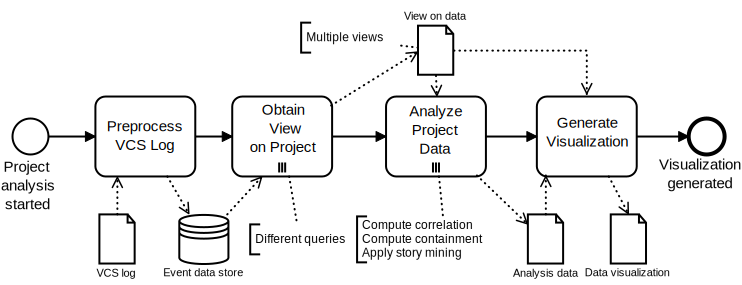
\includegraphics[width=.8\textwidth]{figures/visualization-process}
\caption[Generation of a process visualization from VCS logs]{Generation of a process visualization from VCS logs}
\label{fig:visualization-process}
\end{figure}

The first step of the approach is the preprocessing of the \gls{vcs} log received as input. The main goal of this phase is generate a set of events and store them into a database. Second, we obtain different views on the stored events. In particular, we are interested in observing
\begin{inparaenum}[\itshape i)]
	\item all the commits that affected the files over time;
	\item the amount of change brought by the commits to the files; and
	\item the users who issued such commits.
\end{inparaenum}
The third phase is responsible for considering the different perspectives defined by the project manager and through the generated views extract the necessary knowledge. The last phase is responsible for providing the visualization combining the different perspectives considered. In the following, we detail the formal concepts and the algorithm of our technique.

%\subsubsection{Preprocessing VCS Logs.}
%Version control system logs hold rich information about the artifacts and their evolution. Therefore, our process starts by extracting the elements \emph{Artifact}, \emph{Commit} and \emph{Event} from the log.
%
%First, the tree file is analyzed so the \emph{Parent} relation is defined. For that, the artifacts names appearing in the log are used. They provide the whole path from the root file until the leave file, which is the artifact in question. Thus, a parser can analyses the path and create the relation between the files. For instance, suppose we have the artifact \texttt{running example/software/model.java}. Three files are observed from this name: $f_1 = running \quad example$, $f_2 = software$ and $f_3 = model.java$. The following pairs will be included in the \emph{Parent} relation $\{(f_1,f_2),(f_2,f_3)\}$. 
%%are in the same containment if they share a common prefix that is maximal, i.e. they differ only by the name. For example, the files 
%%and \texttt{running example/software/test.java} . belong to the same containment, whereas the files  \texttt{running example/software/model.java} and \texttt{README.md} belong to two different containments. Note that containments can be contained in other containments, therefore every two files with eventually belong to the same containment. 
%
%Second, artifacts are extracted, as specified in Definition \ref{def_artifact}. Then the commits, following Definition \ref{def_commit}, are extracted. At last, the VCS raw log is transformed into a list of events for the extracted artifacts and commits, as specified in Definition \ref{def_event}. This step is easily done by replicating the information on commit level to be contained in the events. The amount of change is determined analyzing the attribute Diff of the VCS log. For instance, commit ID 2 in Table \ref{tab:vcs-log-data} indicates a commit with amount of change equals 3. The output of this phase is a set of events $E$, a set of artifacts $A$ and a set of commits $Com$.
%
%\subsubsection{Obtain View on Project.}
%The main goal of this phase is to extract the data that will be analyzed. The focus of this paper is in the artifacts, therefore the views generated gather information about events related to artifacts.  
%
%The project manager must determine the level of detail for the analyzes, thus, specifying the time windows. Input parameters of this phase are the interval of analysis ($ia$) and the time window for aggregation ($tw_{agg}$). Considering the specified $tw_{agg}$, the events generated in the previous phase are aggregated. For each artifact in a particular aggregate time an \emph{Aggregate Event} is generated as defined in Definition \ref{def_aggregateEvent}.
%
%\subsubsection{Analyze project data.}
%In this phase, the project is analyzed considering the different perspectives the project manager is interested in. In this paper, we considered three perspectives: dependency between artifacts, containments and artifact evolution.
%
%\paragraph{Dependency.} As stated in \Cref{def_dependency}, a dependency between two artifacts exists if both artifacts require a similar effort to be maintained, i.e. if they have a similar behavior considering the amount of changes.  The amount of change of an artifact over time defines  a time series. Therefore, for each artifact its aggregate events are analyzed in order to extract the amount of change for each aggregated time towards defining a time series for this artifact. 
%
%Let $AE$ be the set of aggregate events within $ia$. We build the time series for the \emph{i}-th artifact, namely $X_{f_i} = \lbrace (t, c) ~|~ e_a \in AE,~ t = ats(e_a),~ c = aac(e_a),~ f(e_a) = {f_i} \rbrace $. 
%
%%\todo[inline]{
%%Dependencies are obtained from the aggregated events. Considering the time window $tw$ and the aggregated event set in that time window ($AE_{tw}$), %$AE' = \lbrace e~|~ e \in AE,~ ts(e) \in tw \rbrace$,
%%we build the time series for the \emph{i}-th artifact, namely $X_{f_i} = \lbrace (t, c) ~|~ e_a \in AE_{tw},~ t = ats(e_a),~ t \in tw,~ c = aac(e_a),~ f(e_a) = {f_i} \rbrace $. As a result, the dependency between \emph{i}-th and the \emph{j}-th artifact is the correlation across time series $\sigma(i,j) = {corr(X_i, X_j)}$.
%%}
%
%After the time serie for each artifact is defined, the correlation function is used to calculate the correlation between the two time series. Considering artifacts $f_i$ and $f_j$ and the time series correspondent $X_{f_i}$ and $X_{f_j}$, $\sigma(f_i,f_j) = {corr(X_{f_i}, X_{f_j})}$ is the correlation value found when applying correlation function $corr$.
%
%If $\sigma(f_i,f_j)$ overcomes a threshold defined by the project manager (input parameter of this phase), then a dependency between the correspondent artifacts is established. The strength of the dependency is defined by $\sigma(f_i,f_j)$. 
%
%\paragraph{Containments.}
%For the containments extraction, the $Parent$ relation is analyzed and the set $C$ of containments defined.
%Containments reflect the hierarchical nature of the file structure in a repository. That is, \emph{composite containments} can be recursively decomposed into smaller containments until an \emph{atomic containment} is reached, following the tree structure of the file system top down. Conversely, from navigating the file structure bottom up, containments can be part of other containments until the root containment is reached. 
%
%
%\paragraph{Artifact evolution.}
%%For the artifact evolution definition, we propose to apply story mining techniques as follows.
%
%\input{sections/file-mining}

 %\hfill\\
%1. Compute correlation - dependency
%2. Compute containments 
%3. Apply story mining to obtain the process  - artifact evolution \\\hfill

%\subsubsection{Generate visualization.}
%%The approach is flexible making possible to generate different visualizations 
%In this section, we define the graphical elements of the visualization and their semantic. 
%
%%\input{table/visual-symbols}
%\paragraph{Project Participant.}
%%\todo[inline]{Task was not defined before. I think in our case workload will be in how many changes the project participant is involved within a period of time. I change to this idea. See what do you think. \\[2pt] I also consider project participant instead of resource following what was defined in section II.A. But I am ok with both. We just need to decide and change the whole paper. \\[2pt] The symbols have different faces and the semantic was not provided. I know they align with the color, but I think it is better to have the same face (not all people with high workload are sad or with low workload are happy). On the other hand, we lost the representation of a participant in the process, i.e. we are not able to visualize how many different participant worked in the same process (artifact). If we are still interested in that, I suggest to leave the faces as symbolizing the workload and the colors to symbolize different participants}
%
%Project Participants are displayed through a face symbol with its identification in the top, as depicted in  \Cref{fig:resources}. We use a color code to denote their level of workload, i.e. in how many changes the project participant is involved in the project within $ia$. \emph{Red}, \emph{yellow} and \emph{green} color indicate \emph{high}, \emph{medium} and \emph{low} project workload respectively. The project workload for a project participant ($wl_u$) is computed from the set of events in which the project participant was responsible for the change within $ia$, i.e. $wl_u(t_1,t_2) = |\lbrace e \in E ~|~  u(e)= u, t_1 \leq ts(e) \leq t_2 \rbrace|$, where $ia=[t_1 , t_2]$. These interval of analysis can be fine tuned to visualize the project participant occupancy over time. 
%
%%\begin{figure}[h]
%%	\centering
%%	\begin{subfigure}{.3\linewidth}
%%		\centering
%%		\begin{tikzpicture}[scale=.2]
%%		\node[text width=3cm] at (2,2.3) {resource};
%%		
%%		\filldraw [color=black, fill=green!50] (0,0) circle (2);
%%		\filldraw [color=black, fill=white] (-0.5,.6) ellipse (0.2 and 0.6);
%%		\filldraw [color=black, fill=white] (0.5,.6) ellipse (0.2 and 0.6);
%%		\filldraw [color=black, fill=black] (-0.5,.4) ellipse (0.2 and 0.3);
%%		\filldraw [color=black, fill=black] (0.5,.4) ellipse (0.2 and 0.3);
%%		\draw  (-1,-0.5) .. controls (-0.5,-1) and (0.5,-1) .. (1,-0.5);
%%		\draw  (-1,-0.5) .. controls (-0.5,-1.3) and (0.5,-1.3) .. (1,-0.5);
%%		\fill[fill=white, draw=black, opacity=1] (-1,-0.5) .. controls (-0.5,-1) and (0.5,-1) .. (1,-0.5) .. controls (0.5,-1.3) and (-0.5,-1.3) .. (-1,-0.5) --cycle;
%%		\end{tikzpicture}
%%		%		
\includegraphics[width=.3\linewidth]{figures/visualization-elements/green-face}
%%		\caption{}
%%		\label{fig:green}
%%	\end{subfigure}%
%%	\begin{subfigure}{.3\linewidth}
%%		\centering
%%		%		
\includegraphics[width=.3\linewidth]{figures/visualization-elements/yellow-face}
%%		\begin{tikzpicture}[scale=.2]
%%		\filldraw [color=black, fill=yellow!50] (0,0) circle (2);
%%		\filldraw [color=black, fill=white] (-0.5,.6) ellipse (0.2 and 0.6);
%%		\filldraw [color=black, fill=white] (0.5,.6) ellipse (0.2 and 0.6);
%%		\filldraw [color=black, fill=black] (-0.5,.4) ellipse (0.2 and 0.3);
%%		\filldraw [color=black, fill=black] (0.5,.4) ellipse (0.2 and 0.3);
%%		%mouth
%%		%		\draw  (-1,-0.6) .. controls (-0.5,-1) and (0.5,-1) .. (1,-0.5);
%%		%	\draw  (-1,-0.5) .. controls (-0.5,-1.3) and (0.5,-1.3) .. (1,-0.5);
%%		\fill[fill=white, draw=black, opacity=1] (-1,-0.7) .. controls (-0.5,-0.8) and (0.5,-0.8) .. (1,-0.7) .. controls (0.5,-1) and (-0.5,-1) .. (-1,-0.7) --cycle;
%%		\end{tikzpicture}
%%		\caption{}
%%		\label{fig:yellow}
%%	\end{subfigure}%
%%	\begin{subfigure}{.3\linewidth}
%%		\centering
%%		%		\includegraphics[width=.3\linewidth]{figures/visualization-elements/red-face}
%%		\begin{tikzpicture}[scale=.2]
%%		\filldraw [color=black, fill=red!60] (0,0) circle (2);
%%		\filldraw [color=black, fill=white] (-0.5,.6) ellipse (0.2 and 0.6);
%%		\filldraw [color=black, fill=white] (0.5,.6) ellipse (0.2 and 0.6);
%%		\filldraw [color=black, fill=black] (-0.5,.4) ellipse (0.2 and 0.3);
%%		\filldraw [color=black, fill=black] (0.5,.4) ellipse (0.2 and 0.3);
%%		%			\draw  (-1,-0.5) .. controls (-0.5,-1) and (0.5,-1) .. (1,-0.5);
%%		%		\draw  (-1,-0.5) .. controls (-0.5,-1.3) and (0.5,-1.3) .. (1,-0.5);
%%		\fill[fill=white, draw=black, opacity=1] (-1,-1) .. controls (-0.5,-0.5) and (0.5,-0.5) .. (1,-1) .. controls (0.5,-0.8) and (-0.5,-0.8) .. (-1,-1) --cycle;
%%		\end{tikzpicture}
%%		\caption{}
%%		\label{fig:red}
%%	\end{subfigure}
%%	\caption{Project Participant symbols. Color codes represent the status of their workload within a period of time.}
%%	\label{fig:resources}
%%\end{figure}
%
%
%%\begin{figure}[h]
%%	\centering
%%		\begin{tikzpicture}[scale=.2]
%%		\node[] at (0,3.5) {\textit{participant}};
%%		\filldraw [color=black, fill=white!50] (0,0) circle (2);
%%		\filldraw [color=black, fill=white] (-0.5,.6) ellipse (0.2 and 0.6);
%%		\filldraw [color=black, fill=white] (0.5,.6) ellipse (0.2 and 0.6);
%%		\filldraw [color=black, fill=black] (-0.5,.4) ellipse (0.2 and 0.3);
%%		\filldraw [color=black, fill=black] (0.5,.4) ellipse (0.2 and 0.3);
%%		%mouth
%%		%		\draw  (-1,-0.6) .. controls (-0.5,-1) and (0.5,-1) .. (1,-0.5);
%%		%	\draw  (-1,-0.5) .. controls (-0.5,-1.3) and (0.5,-1.3) .. (1,-0.5);
%%		\fill[fill=white, draw=black, opacity=1] (-1,-0.7) .. controls (-0.5,-0.8) and (0.5,-0.8) .. (1,-0.7) .. controls (0.5,-1) and (-0.5,-1) .. (-1,-0.7) --cycle;
%%		\end{tikzpicture}
%%	\caption{Project Participant symbol. The workload within a period of time is color coded.} 
%%	\label{fig:resources}
%%\end{figure}
%
%
%
%\paragraph{Dependency.}
%A dependency between two artifacts is represented by a line that connects their atomic containments. We label dependencies with a number  $\sigma \in \Re$, which indicates the strength of the dependency among the two artifacts. \Cref{fig:dependency} illustrate the notation for dependencies.
%
%%\begin{figure}[h]
%%	\centering
%%	%	\includegraphics[width=0.7\linewidth]{figures/visualization-elements/dependency}
%%	\begin{tikzpicture}[scale=.5]
%%	\draw[thick] (-2,0) -- node[above,thick] {$\sigma$} ++(4,0);
%%	\end{tikzpicture}
%%	\caption{Dependency with strength $\sigma$}
%%	\label{fig:dependency}
%%\end{figure}
%
%\paragraph{Artifact evolution.}
%
%The artifact evolution is a process under which the artifact changes step by step towards a final state reached eventually in the project (e.g. a documentation file reaches his final state when the documentation is complete and no edits are made to that version of document anymore). Thus, we chose the \gls{bpmn} to represent this process. 
%
%\Cref{fig:process} depicts an example of a process learned considering a story with two aggregated comments, thus a process with two sequential activities \emph{a} and \emph{b}, modeled in \gls{bpmn}. 
%
%%\tikzstyle{startstop} = [rectangle, rounded corners, minimum width=1.5cm, minimum height=1cm,text centered, draw=black, fill=white!30]
%%\tikzstyle{arrow} = [thick,->,-latex]
%%\tikzstyle{event} = [circle,scale=.5, minimum width=1cm, minimum height=1cm,draw,fill=white]
%%\tikzstyle{end event} = [event,ultra thick]
%%
%%\begin{figure}[h]
%%	\centering
%%	%
\includegraphics[width=0.7\linewidth]{figures/visualization-elements/process}
%%	\begin{tikzpicture}[scale=.3]
%%	\begin{scope}[auto, every node/.style={draw,circle},node distance=.2cm]
%%	\node (start) [event] {};
%%	\node (add) [startstop, right of=start, xshift=1.3cm] {a};
%%	\node (fix) [startstop, right of=add, xshift=1.9cm] {b};
%%	\node (end) [end event, right of=fix, xshift=2.8cm] {};
%%	\draw [arrow]  (start) -- (add);
%%	\draw [arrow]  (add) -- (fix);
%%	\draw [arrow]  (fix) -- (end);
%%	\end{scope}
%%	\end{tikzpicture}
%%	\caption{Process representing an artifact evolution using \gls{bpmn}.}
%%	\label{fig:process}
%%\end{figure}
%
%
%\paragraph{Containment.} 
%A containment is represented with a rectangle. 
%We overload the semantic of rectangle used to represent the containment with a time concept. The position of the \emph{atomic containments} is shifted within the boundaries of their parent containments according to the first timestamp of the artifact history. For example, given two \emph{atomic containments} $C_1\{f_i\}$, $C_2\{f_j\} \subseteq C$, and let $AE_i, AE_j \subseteq AE$ be the sets of aggregated events that affected these artifacts, respectively. Then $C_1$ is shifted left with respect to $C_2$ if $min\{ats(e) | e \in AE_i\} < min\{ats(e') | e' \in AE_j\}$. \Cref{fig:containment} illustrates this example.
%
%%\begin{figure}[h]
%%\centering
%%%\includegraphics[width=0.7\linewidth]{figures/visualization-elements/containment}
%%\usetikzlibrary{
%%	shapes.geometric,
%%	positioning,
%%	fit,
%%	calc
%%}
%%\begin{tikzpicture}
%%	\draw[thick] (0,0)rectangle (4,2) node[pos=.85] {$C_3$};
%%	\draw[thick] (1.1,1.1) rectangle (2.2,1.6) node[midway] {$C_1$}; 
%%	\draw[thick] (2.1,0.1) rectangle (3.2,0.6) node[midway] {$C_2$};
%%\end{tikzpicture}
%%\caption{A containment $C_3$ composed of two atomic containments $C_1$, $C_2$. $C_1$ is shifted more left wrt $C_2$ as its contained artifacts were affected by changes earlier.}
%%\label{fig:containment}
%%\end{figure}
%
%\begin{figure}
%	\centering
%	\begin{subfigure}[t]{.5\textwidth}
%		\centering
%		\begin{tikzpicture}[scale=.2]
%		\node[] at (0,3.5) {\textit{participant}};
%		\filldraw [color=black, fill=white!50] (0,0) circle (2);
%		\filldraw [color=black, fill=white] (-0.5,.6) ellipse (0.2 and 0.6);
%		\filldraw [color=black, fill=white] (0.5,.6) ellipse (0.2 and 0.6);
%		\filldraw [color=black, fill=black] (-0.5,.4) ellipse (0.2 and 0.3);
%		\filldraw [color=black, fill=black] (0.5,.4) ellipse (0.2 and 0.3);
%		%mouth
%		%		\draw  (-1,-0.6) .. controls (-0.5,-1) and (0.5,-1) .. (1,-0.5);
%		%	\draw  (-1,-0.5) .. controls (-0.5,-1.3) and (0.5,-1.3) .. (1,-0.5);
%		\fill[fill=white, draw=black, opacity=1] (-1,-0.7) .. controls (-0.5,-0.8) and (0.5,-0.8) .. (1,-0.7) .. controls (0.5,-1) and (-0.5,-1) .. (-1,-0.7) --cycle;
%		\end{tikzpicture}
%		\caption{Project Participant symbol. The workload within a period of time is color coded.} 
%		\label{fig:resources}
%	\end{subfigure}~
%	\begin{subfigure}[t]{.5\textwidth}
%		\centering
%		%	\includegraphics[width=0.7\linewidth]{figures/visualization-elements/dependency}
%		\begin{tikzpicture}[scale=.5]
%		\draw[thick] (-2,0) -- node[above,thick] {$\sigma$} ++(4,0);
%		\end{tikzpicture}
%		\caption{Dependency with strength $\sigma$}
%		\label{fig:dependency}
%	\end{subfigure}\\
%	\begin{subfigure}[t]{.5\textwidth}
%		\tikzstyle{startstop} = [rectangle, rounded corners, minimum width=1.1cm, minimum height=.6cm,text centered, draw=black, fill=white!30]
%		\tikzstyle{arrow} = [thick,->,-latex]
%		\tikzstyle{event} = [circle,scale=.7, minimum width=.5cm, minimum height=.5cm,draw,fill=white]
%		\tikzstyle{end event} = [event,ultra thick]
%		%		\begin{figure}[h]
%		\centering
%		%
\includegraphics[width=0.7\linewidth]{figures/visualization-elements/process}
%		\begin{tikzpicture}
%		\begin{scope}[auto, every node/.style={draw,circle},node distance=.05cm]
%		\node (start) [event] {};
%		\node (add) [startstop, right of=start, xshift=1cm] {a};
%		\node (fix) [startstop, right of=add, xshift=1.5cm] {b};
%		\node (end) [end event, right of=fix, xshift=1.6cm] {};
%		\draw [arrow]  (start) -- (add);
%		\draw [arrow]  (add) -- (fix);
%		\draw [arrow]  (fix) -- (end);
%		\end{scope}
%		\end{tikzpicture}
%		\caption{Process representing an artifact evolution using \gls{bpmn}.}
%		\label{fig:process}
%		%		\end{figure}
%	\end{subfigure}~~
%	\begin{subfigure}[t]{.45\textwidth}
%		\centering
%		%\includegraphics[width=0.7\linewidth]{figures/visualization-elements/containment}
%		\usetikzlibrary{
%			shapes.geometric,
%			positioning,
%			fit,
%			calc
%		}
%		\begin{tikzpicture}[scale=.99]
%		\draw[thick] (0,0)rectangle (4,2) node[pos=.85] {$C_3$};
%		\draw[thick] (1.1,1.1) rectangle (2.2,1.6) node[midway] {$C_1$}; 
%		\draw[thick] (2.1,0.1) rectangle (3.2,0.6) node[midway] {$C_2$};
%		\end{tikzpicture}
%		\caption{A containment $C_3$ composed of two atomic containments $C_1$, $C_2$. $C_1$ is shifted more left wrt $C_2$ as its contained artifacts were affected by changes earlier.}
%		\label{fig:containment}
%	\end{subfigure}
%	\caption{Graphic elements used to represent the defined concepts of project participant, work dependency, artifact evolution and containment.}
%\end{figure}
%
%\paragraph{Composing the visualization.}
%
%The layout rules to compose the visualization are the following. 
%\begin{inparaenum}[\itshape (i)]
%	\item Every element is within a containment, excluding the root;
%	\item Project participants responsible for the change are placed over \gls{bpmn} activities;
%	\item Artifact evolution is within an atomic containment;
%	\item Dependencies connect atomic containments, showing the strength of correlations between the belonging artifacts evolutions.
%\end{inparaenum}
%\Cref{fig:all-elements-together} shows the correct composition of the presented visual elements.
%
%\begin{figure}
%\centering
%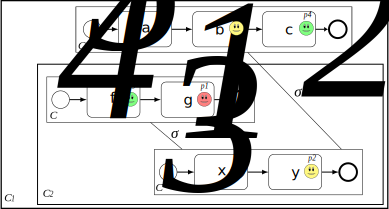
\includegraphics[width=.6\linewidth]{figures/visualization-elements/al-elements-together}
%\caption{Composition of the graphic elements into five containments, of which two are composite.}
%\label{fig:all-elements-together}
%\end{figure}



\subsection{Preliminaries}
\label{subsec:prelim}

%1. How we define/capture software processes\\

%2. How we define containment\\

%3. How we define dependencies\\

%Version control systems (VCSs) are used in projects to ensure reliable collaboration. We build our technique on \gls{vcs}. Typically, people work in VCS on files (e.g., text, source code, spread sheets) and commit them to the central repository. Project participants comment on their commits so that other participants can better understand the nature of the changes performed to the files.

As the objective of our technique is to uncover hidden work dependencies, we define the fundamental concepts required to capture them. Work is reflected by \emph{artifacts}, e.g., word documents, spreadsheets, code, etc. Artifacts are leaves in the file tree hierarchy (with directories being special type of non-leaf files). %Each directory in the file system groups together one or more files into a so-called \emph{containment}. 
Artifacts evolve over time, while project participants contribute their changes. Each change is an \emph{event} that happens to an artifact in a single point in time. Events can be abstracted into \emph{aggregated events} that allow a coarser grained view on the history. The history of the changes of an artifact over a time interval at a given level of abstraction is referred to as \emph{artifact evolution}. Similar artifact co-evolution establishes a \emph{dependency} between two artifacts. %In the following, we formally define the aforementioned concepts.

A software product is subdivided into files and directories. In this work, we consider directories as special type of files which are parents of other files. Formally, let $F$ be the universe of files in a software development project. Files are organized in a file tree. Therefore, each file $f \in F$ has one parent file. The only file without a parent file is the \emph{root} file. We capture this information in the parent relation $Parent: F \times F$. For example, let $f_p \in F$ be the parent of file $f_c \in F$, then $(f_p, f_c) \in Parent$. %Every file in $Parent$ defines a so-called \emph{containment}. For example, let $Parent = \{(f_{p_1} , f_{c_1})$, $(f_{p_1},f_{c_2})$, $(f_{p_2},f_{c_3})$, $(f_{p_3},f_{p_1})$,$(f_{p_3},f_{p_2})\}$, then files $f_{p_1}$, $f_{p_2}$ and $f_{p_3}$ define containments. Let $C$ be the set of containments. In our example $C=\{f_{p_1}, f_{p_2}, f_{p_3}\}$.
An \emph{artifact} is a file that is not a parent file, i.e. a file $f_a$ is an artifact if $\forall_{f \in F} (f_a, f) \notin Parent$.

%In this work, we are interested in describing the work progress related to a specific file, that we henceforth call \emph{artifact} and describe as follows:

%\begin{definition}
%	\label{def_artifact}
%	{\bf (Artifact)} An \emph{artifact} is a file that it is not a parent file, i.e. a file $f_a$ is an artifact if $\forall_{f \in F} (f_a, f) \notin Parent$.
%\end{definition}
%
%The files are grouped considering their organization in the tree file. We call each of these groups \emph{containments} and they are defined as follows:
%\begin{definition}
%\label{def_containment}
%{\bf (Containment)} A \emph{containment} is a file that is a parent of at least one other file. For example, let $Parent = \{(f_{p_1} , f_{c_1})$, $(f_{p_1},f_{c_2})$, $(f_{p_2},f_{c_3})$, $(f_{p_3},f_{p_1})$,$(f_{p_3},f_{p_2})\}$, then files $f_{p_1}$, $f_{p_2}$ and $f_{p_3}$ are containments. Let $C$ be the set of containments. In our example $C=\{f_{p_1}, f_{p_2}, f_{p_3}\}$.
%\end{definition}

%\begin{definition}
%	\label{def_artifact}
%	{\bf (File Containment)} An \emph{artifact} is a file that it is not a parent file, i.e. a file $f_a$ is an artifact if $\forall_{f \in F} (f_a, f) \notin Parent$.
%\end{definition}


%Containments can be either \emph{atomic} or \emph{composite}. An \emph{atomic containment} is a file which is parent of artifacts. In our example, containments $f_{p_1}$ and  $f_{p_2}$ are atomic containments.
%%\Cref{fig:containment} shows the visual symbol for an atomic containment.
%A \emph{composite containment} is a containment which is not atomic, i.e. it involves files which are parents of parents. In our example, containment $f_{p_3}$ is a \emph{composite containment}.  Therefore, the set $C$ of containments is partitioned in two subsets $C=C_1 \cup C_2$. In our example, $C=\{\{f_{p_1}, f_{p_2}\},\{f_{p_3}\}\}$.


% are defined, $C_1 = \{f_{c_1},f_{c_2}\}$ and $C_2=\{f_{c_3}\}$. A \emph{containment} $C$ is a set of files with the same parent file. For example, let $Parent = \{(f_{p_1} , f_{c_1}), (f_{p_1},f_{c_2}), (f_{p_2},f_{c_3})\}$, then two containments are defined, $C_1 = \{f_{c_1},f_{c_2}\}$ and $C_2=\{f_{c_3}\}$.

When project participants do a certain amount of work and want to save their current progress, they commit the changes to the \gls{vcs}. We define changes on artifacts as the \emph{events} of interest on the lowest granularity.

\begin{definition} {\bf(Event)}
\label{def_event}
Let $E$ be the set of events. An \emph{event} $e \in E$ is a five-tuple $(f, ac, ts, k,u)$, where
\begin{itemize}
\item $f \in F$ is the affected artifact of the event.
%\item $o \in O$ = \{added, modified, deleted\} is the change operation on the artifact with obvious meaning.
\item $ac \in AC =  \mathbb{N}$ is the amount of change done in the artifact.
\item $ts \in TS = \mathbb{N}$ represents a unix time stamp marking the time of the event occurrence.
\item $k \in \Sigma ^* $ is a comment in natural language text.
\item $u \in U$ is the project participant responsible for the change.
\end{itemize}
\end{definition}

For event $e = (f, ac, ts, k,u)$ we overload $f$, $ac$, $ts$, $k$ and $u$ to be used as accessor functions. For example, $f$ is the function $f : E \rightarrow F$ mapping an event to its affected artifact.

In some situations, it can be interesting to have a higher level overview of the changes done to a particular artifact. In this case, an aggregation of events related to this artifact in an interval of time can be performed. The time window for the aggregation, henceforth denoted as $tw_{agg}$, must be defined, i.e. the size of the time interval. For instance, a time window for aggregation can be a day. Thus, all events occurring for an artifact in the same day will be aggregated. An \emph{aggregated event} is defined as follows:

\begin{definition} {\bf (Aggregated Event)}
\label{def_aggregateEvent}
An \emph{Aggregated Event} for $tw_{agg}$ ($AE_{tw_{agg}}$) is a five-tuple $(f, aac, ats, ak,au)$, where
\begin{itemize}
\item $f \in F$ is the affected artifact in the set of events being aggregated.
%\item $ao \in O$ = \{added, modified, deleted\} is the aggregated change operation on the artifact. If the only change operation performed in $tw_{agg}$ was \emph{added} or \emph{deleted} then the aggregated change operation is the same, otherwise it is \emph{modified}.
\item $aac \in AAC =  \mathbb{N}$ is the aggregate amount of change done in the artifact for $tw_{agg}$. It is calculated by summing the amount of changes done in each of the time aggregated.
\item $ats \in ATS = \mathbb{N}$ represents an aggregate time of the unix time stamp of the events being aggregated.
\item $ak \in \Sigma ^* $ is the concatenation of the comments presented in the events being aggregated.
\item $au \subseteq U$ are the project participants responsible for the changes in $tw_{agg}$ being aggregated.
\end{itemize}
\end{definition}
%\todo[inline]{We consider a $tw$ but do not use it in the definition.}

The set of aggregated events for a particular artifact defines how this artifact evolves over time. Considering an interval of analysis, henceforth denoted as $ia$, we define artifact evolution as follows.

\begin{definition} {\bf (Artifact Evolution)}
%Let $EA_f$ be the set of all aggregated events related to artifact $f$.
\emph{Artifact evolution} is the process describing how the file $f$ changed over an interval of time $ia$, i.e., a set of labeled tuples $A_{evo}(f) = \{ (t,a,l) | e \in AE_{ia}, f=f(e), t=ats(e), a=aac, l=ak(e)\}$ chronologically ordered.

%The comments associated to the aggregated events in $EA_f$ define the activities executed. The time of the aggregated events in $EA_f$ establishes the order of the activities and then the flow of evolution. Each activity is associated with the user that executed it.
\end{definition}

%Project participants can commit a number of changes to different artifacts at one step. Therefore, we define the notion of commits as follows.
%
%\begin{definition} {\bf (Commit)}
%\label{def_commit}
%A \emph{commit} $Com$ is a set of events sharing the same time stamp and comment, i.e., $\forall e, e'\in Com : ts(e) = ts(e')\wedge k(e) = k(e')$. Additionally, each event in a commit affects different artifact, i.e., $\forall e, e' \in Com : e \neq e' \rightarrow f(e) \neq f(e')$.
%\end{definition}

%For example, a dependency is established if the two artifacts require a similar effort to be maintained. The effort of maintenance is measured through the amount of changes done to the artifact.

%\begin{definition} {\bf (Dependency)}
%\label{def_dependency}
%A \emph{dependency} between two artifacts within $ia$ is a similarity function $\sigma : X_{evo} \times X_{evo} \rightarrow \mathbb{Z}$, where the artifact evolution set in which the labels are projected out, i.e $X_{evo} = \{(t,a) | \exists l : (t,a,l) \in A_{evo}\}$.
%%Thus, each artifact defines a time series of the amount of change. If the correlation between two time series is significant then a dependency between the correspondent artifacts is established. The strength of the dependency is defined by the correlation value.
%\end{definition}
%
%
%
%\subsection{Metrics} 

Note that artifact evolution represents the changes that happened to a file over time. Thus, we can build the time series of a file $f$ as the vectors of changes $\vec{X_{f}} = (a_1, ..., a_n)$ in the time window $tw_{agg} = [t_1,t_n]$, with $a_i$ being the sum of the changes of $f$ in of the aggregated intervals $t_i$ of the time window $tw_{agg}$.

%The file system establishes a structural tree-based relationship among files. However, other types of dependencies can emerge between two files. In this paper, we define dependency between two files in terms of their \emph{degree of co-evolution}.
%In this paper, we are interested in measuring the hidden work-dependencies among artifacts of the project-oriented business process. That is, we want to capture dependencies that are created among files that go beyond functional (e.g. interface-implementing class) or structural (e.g., parent-child in the file tree structure).

%We define the metrics of \emph{degree of co-evolution} and \emph{file distance}. 

We measure the dependency between two files $f_a$ and $f_b$ in terms of their \emph{degree of co-evolution} as follows.
\begin{definition} {\bf (Degree of Co-Evolution)} 
	\label{definition:degree-of-coevolution}
	Given two files $f_a$ and $f_b$, the \emph{degree of co-evolution} $\chi: F \times F \rightarrow [0,1]$ is a similarity function of the respective time series.
\end{definition}
In this paper, we fix $\chi(f_a,f_b) = |\sigma (\vec{X_{f_a}}, \vec{X_{f_b}})|$, where $\sigma$ is the correlation function of the two vectors $\vec{X_{f_a}}$ and $ \vec{X_{f_b}}$.

The way files are kept in the directory structure establishes an inherent relationship among files being stored close to each other in the hierarchy. For instance, files serving the same purpose are stored close to each other in the file system. 
Hidden work dependencies are expected to happen between artifacts that are distant in the file structure. We measure this distance as the length of the shortest route connecting two files in the file tree. We adapt the notion of path from~\citep{Gubichev2010} to our file tree. Given a file $f$, the path to the root node can be obtained by navigating the $Parent$ relationship up to the root file. The path $p$ from $f_a$ to the root $f_r$ is the set of parent files encountered along such route. i.e. $p(f_1,f_{r}) = \{(f_1, ..., f_k, f_{k+1}, ..., f_{r})\}$ such that for any $k$, $(f_{k+1},f_k) \in Parent $. The length of the path is the cardinality $|p|$ of the set. 
The shortest path between two files $f_a$, $f_b$ in a tree passes through the \gls{lca}~\citep{Bender2000}. This is equivalent to considering the paths from the single files to the root node $p_a = p(f_a,f_r)$ and $p_b=p(f_b, f_r)$ minus their intersection $I_{p_a,p_b}=\{p(f_a, f_r) \cap p(f_b, f_r)\}$. Thus, we define the \emph{file distance} as the length of the shortest path between two files $f_a$ and $f_b$ as follows. 

\begin{definition} {\bf (File Distance)} 
	\label{definition:artifact-distance}
	The distance $d : F \times F \rightarrow \mathbb{N} $ between two files belonging to the same directory structure is defined as the number of nodes in the minimum path connecting the two files in the project file tree: $d(f_a,f_b) =  |p_a| + |p_b| - 2*(|I_{p_a,p_b}|)$.
\end{definition}
 

\subsection{Hidden Dependencies Discovery Algorithm}

We are focused on finding interesting hidden work dependencies. These dependencies are typically reflected by changes that happen to couples of allegedly unrelated files during their evolution. This section details the procedure that implements the technique outlined in \Cref{fig:visualization-process}.

\Cref{algorithm:all} presents the steps required to explicate such hidden dependencies. The procedure $\mathtt{PreprocessLog(\mathcal{L})}$ in line~\ref{step:preprocess} takes as input a VCS log $\mathcal{L}$ structured as in \Cref{tab:vcs-log-data} and parses out work events at the granularity of line changes. These events are then stored into an event data storage. Events parsed from \gls{vcs} logs contain rich information about multiple aspects of the work they reflect. In order to represent all these different aspects, we devised the entity-relationship data model. Hence, we are able to store all the information that is possible to obtain after parsing the \gls{vcs} log. Furthermore, this step allows the user to obtain simple information, such as statistics on the project, already at an early stage of the procedure. The output of the $\mathtt{PreprocessLog(\mathcal{L})}$ step results in the storage of all the events $E$ into a database.
%Further on, we will show a possible implementation that uses a database to store the parsed events, but in principle any type of repository that allows to store the preprocessed events can be considered.

%\begin{figure}
%	\centering
%	\includegraphics[width=.8\textwidth]{figures/CommitLogER3.pdf}
%	\caption{Entity-Relationship model used to store events extracted from VCS logs}
%	\label{fig:data-model}
%\end{figure}


Next, the iterative call of the procedure $\mathtt{RetrieveView(\mathit{E}, \mathsf{query})}$ in line \ref{step:retrieve-view} performs several querying the data storage containing the set $E$. For example, a possible query can obtain all the comments associated to each change of a specific file. To obtain information on the evolution of files, we query the database for the changes of all the files within a user defined time interval $tw_{agg}$. In general several time frames can be chosen, each of them producing a \emph{view} $V$ on the data, i.e., a set of aggregated events chronologically sorted within $tw_{agg}$. For example, users may be interested in artifact-views aggregated by day, by month, etc. Multiple \emph{views} are possible by defining them in the {\textsf{queries}} parameter. We collect these views into a set $\mathcal{V} = \bigcup_{\textsf{queries}} V$. 

%Step~\ref{step:contaiments} extracts the structural relationships among the file paths contained in each view $V$, i.e., it recreates the file tree from the artifacts.


\input{bpm2017/algorithms/all}%\input{algorithms/RetrieveView}
%\Cref{algorithm:compute-containments} computes the containments. Note that both atomic and composite containments are computed.

%\input{algorithms/ComputeContainments}

The step in line~\ref{step:evolution} starts an iteration over the views set $\mathcal{V}$. Here is where we collect the analysis data that are returned by the algorithm. For each of the aggregated artifacts contained in a view $V$, we retrieve the information necessary to compute the \emph{degree of co-evolution} between pairs of files and their \emph{file distance}. First, we construct the artifact evolution of all the artifacts present in $ae \in V$. 
Note that an aggregated event $ae \in V$ is a record obtained from a view on the project which is composed, among other attributes (e.g., file, time, amount of change), by the comment associated to the specific change. Comments describe multiple changes executed on the file, i.e. they describe a \emph{story} of the artifact. 
Stories associated to each file are collected and the corresponding labels are chronologically ordered. These file stories are then input to the StoryMining technique~\cite{Goncalves2011}. Story Mining was designed to receive as input a story freely written by the participants, describing their work in a particular business process. As an output, the \emph{actors} and the process \emph{activities} executed by them are extracted. Our technique is concerned with the stories of the files. Therefore, they are the actors of the story mining, and the resulting business process consists of the steps describing their evolution process. We collect the resulting processes in the step in line~\ref{step:story-mining}.
The step in line~\ref{step:timeseries} is concerned with the construction of a time series from the set of artifact evolutions $A_{evo}$ computed in line~\ref{step:a-evo}. Specifically, this step gathers the values of the changes of each of the artifact $f$ in $A_{evo}$ and records them in $TimeSeries(f)$. 

After all the aggregated events $ae$ have been explored, the algorithm moves on to computing the metrics (lines~\ref{step:metric-start}--\ref{step:metric-end}). In this loop, the algorithm iterates through all the pairs of files. For each pair, the \emph{degree of co-evolution} and \emph{artifact-distance}  metrics are computed according the \Cref{definition:degree-of-coevolution} and \Cref{definition:artifact-distance}, respectively. These two measures are collected only if their values are above the user defined thresholds $\gamma$ and $\delta$. After the loop is over, the two measurements and the stories mined with the StoryMiner are stored in $AnalysisData$.

Finally, after iterating over all the user defined views, the algorithm returns the $AnalysisData$ collection which can now be further inspected and analyzed in more detail, as we show next with an example.

%\input{algorithms/ComputeEvolution}



%\input{algorithms/ComputeDependencies}
%
%The algorithm iterates over the views and creates the time series from the aggregated events $v$ in each of the views $V$ of the view collections $\mathcal{V}$. A time series is captured by a set $X_{f_i}$, recording the trend of the changes of file $f_i$ over the time. Next, the dependencies are calculated by using the similarity function $\sigma$ (cf. \Cref{def_dependency}) pairwise over the time series of the different artifacts. We do not enforce a determined similarity function between time series. The user can adopt a customized time series similarity function or use an existing method from literature (e.g.~\cite{ruohonen2015time}). Because the time series must have equal length, we add missing times $t$ with couples $(t,0)$. These couples denote that the amount of change in $f$ at time $t$ was 0. Finally, we collect the results in the dependencies set $D$ if they are stronger than the threshold $\delta$.



%\input{sections/metrics}


%\subsection{Story Mining}
\label{subsec:story-mining}

%What is story mining and how we use it in our work
Gon\c{c}alves et al.~\cite{Goncalves2011} proposed a story mining approach to extract process elements from stories, i.e. text descriptions written collaboratively by the process participants. A story is a natural way to transmit and share knowledge. Using both natural language (text) and contextual elements (categorization of parts of the story), storytellers can express their experience and viewpoints about the work processes they participate, interact with and/or perceive. Stories have the advantage of reproducing the situations associated with their contexts - the knowledge that is difficult to capture in interviews or mining from Information Systems logs. Since collectively told, a story incorporates a range of perspectives. Business processes instances can also be viewed as stories played by individuals who perform specific roles depending on the circumstances.

Story Mining  \cite{Goncalves2011} receives as input a story freely written by the participants, describing their work in a particular business process. As an output, the \emph{actors} and the process \emph{activities} executed by them are extracted. To illustrate the approach consider the following story. The terms highlighted in {\bf bold} are the actors of the processes and the terms highlighted in {\color{gray} gray} the activities. 

\begin{figure}[!h]
{ \bf The system} {\color{gray} generates an estimating template consisting of the phases, activities and tasks} selected
for the project or project phase. When planning complete projects the estimating is typically done at the activity level, using the
list of tasks in the work breakdown as input to the estimating process. However {\bf estimators} will likely {\color{gray}add an itemized list of system functions and other deliverables}, to facilitate estimating the construction phase. {\bf Multiple estimators} {\color{gray} prepare estimates for each component}, {\color{gray}compare their estimates}, and {\color{gray}arrive at a final estimate} for each item.
  \label{RB}
\end{figure}

A further step that we developed in our approach is the identification of the relationship between the activities, therefore defining the flow.

%\subsection{Project Mining Software Projects}
\label{subsec:proj-mining}

Project mining technique 


%\section{Evaluation}
\label{sec:evaluation}

In this section, we show the applicability of our technique to project-oriented business processes and its effectiveness in uncovering work dependencies. With respect to the requirements formulated in \Cref{sec:background}, we evaluate against requirements {R2} and {R3} in \Cref{subsec:quantitative-eval} and against requirement {R1} in \Cref{subsec:qualitative-eval}.

We implemented our techniques as a prototype\footnote{The source code is available at \url{https://github.com/s41m1r/MiningVCS}} and used it on 10 real world software projects with different sizes. The input of our program is a \gls{vcs} log and the output is a set of analysis data with information about the evolution of the artifacts and their dependencies. We report the results in \Cref{table:evaluation-results-new}. The results are listed in increasing order of project size. The parameters $\chi$ and $d$ are the metrics of \emph{degree of co-evolution} and \emph{distance}, respectively. In this example, $\chi > 0.7$ signifies that the co-evolution is high ($\chi^{H}$) and $\chi < 0.3$ that the co-evolution is low ($\chi^{L}$). As previously mentioned, this is a user customizable threshold that can be set by the domain expert. Likewise, the distance is considered low ($d^{L}$) when $d<=2$ and high ($d^{H}$) when $d>2$. The parameter  $\overline{|p_f|}$ and {$max(|p_{f}|)$} are respectively the average and the maximum lengths of the path to the root (i.e. average tree depth of the files). The column {$|A_{evo}|$} shows the average number of activities in the process representing the artifact evolution. Lastly, the columns {$\overline{d}$} and {$max(d)$} report the average and maximum file distance, respectively. Next, we use these data for a quantitative evaluation of the projects.

% Please add the following required packages to your document preamble:
% \usepackage{graphicx}
\begin{table}[t]
\centering
\caption[Evaluation on project metric on real world projects.]{Evaluation of real world projects. Respectively the thresholds are: $\chi^{L}$ if $\chi < 0.3$,  $\chi^{H}$ if $\chi > 0.7$  low and high degree of co-evolution; $d^{L}$ if $d \leq 2$,  $d^{H}$ if $d > 2$ respectively low and high distance.}
\label{table:evaluation-results-new}
\resizebox{\textwidth}{!}{%
\begin{tabular}{rrrrrrrrrrrrrr}
Project                 & \rot{Commits} & \rot{Files} & \rot{$\chi^{H}$} & \rot{$\chi^{L}$} & \begin{tabular}[b]{@{}r@{}}{\rot{$(d^{L},\chi^{L})$}}\end{tabular} & \begin{tabular}[b]{@{}r@{}}{\rot{$(d^{L},\chi^{H})$}}\end{tabular} & \begin{tabular}[b]{@{}r@{}}{\rot{$(d^{H},\chi^{L},)$}}\end{tabular} & \begin{tabular}[b]{@{}r@{}}{\rot{$(d^{H},\chi^{H})$}}\end{tabular} & \rot{$\overline{|p_f|}$} & \rot{$max(|p_{f}|)$} & \rot{$|A_{evo}|$} & \rot{$\overline{d}$} & \rot{$max(d)$} \\ \midrule
%smsr                    & 21        & 6         & 22                   & 6                  & 0                          & 9                            & 6                       & 13                        & 2.71             & 5             & 1.82                    & 1.43                & 6                  \\
mwaligner  & 21      & 9     & 37                   & 7                 & 6                               & 30                                 & 1                                          & 7                                             & 1.11              & 2           & 2.40         & 0.94                 & 3                 \\
Biglist                 & 202     & 15    & 22                   & 90                & 31                              & 18                                 & 59                                         & 4                                             & 1.47              & 3            & 2.76         & 1.20                 & 5                 \\
camundaRD & 11      & 15    & 74                   & 26                & 0                               & 25                                 & 26                                         & 49                                            & 2.18              & 4            & 2.05         & 2.03                 & 7                 \\
graphql                 & 256     & 30    & 89                   & 357               & 121                             & 89                                 & 236                                        & 0                                             & 1.40              & 2            & 3.18         & 1.11                 & 4                 \\
jgitcookbook            & 135     & 89    & 773                  & 2866              & 505                             & 289                                & 2361                                       & 484                                           & 6.93              & 8            & 1.33         & 2.68                 & 14                \\
mysqlpython             & 749     & 168   & 2288                 & 11571             & 742                             & 591                                & 10829                                      & 1697                                          & 2.59              & 7            & 1.65         & 2.52                 & 11                \\
gantt                   & 23      & 228   & 7006                 & 14343             & 386                             & 3480                               & 13957                                      & 3526                                          & 3.30              & 4            & 1.71         & 2.16                 & 7                 \\
facebookjavasdk         & 38      & 293   & 16478                & 26092             & 2017                            & 16311                              & 24075                                      & 167                                           & 6.21              & 8            & 4.78         & 5.58                 & 13                \\
caret                   & 864     & 432   & 15366                & 60874             & 9538                            & 14785                              & 51336                                      & 581                                           & 3.01              & 4            & 3.15         & 1.60                 & 7                 \\
operationcode           & 1114    & 1053  & 84024                & 444605            & 2291                            & 5537                               & 442314                                     & 78487                                         & 4.27              & 8            & 2.01         & 4.85                 & 15               \\ \bottomrule
\end{tabular}%
}
\end{table}
%\vspace*{1cm} 

%\subsection{Prototypical Implementation}
\label{subsec:prototype}


%
%The first step of the approach is the preprocess of the VCS log received as input. The main goal of this phase is generate a set of events and store them into a database. Second, we obtain different views on the stored events. In particular, we are interested in observing
%\begin{inparaenum}[\itshape i)]
%	\item all the commits that affected the files over time;
%	\item the amount of change brought by the commits to the files; and
%	\item the users who issued such commits.
%\end{inparaenum}
%The third phase is responsible for considering the different perspectives defined by the project manager and through the generated views extract the necessary knowledge. The last phase is responsible for providing the visualization combining the different perspectives considered. The following sections detail each of the phases.

We implemented our technique as a prototype\footnote{\url{https://github.com/s41m1r/MiningVCS.git}}. The input of our program is a \gls{vcs} log and the output is a set of analysis data with information about the evolution of the artifacts and their dependencies. 
%%Next we show the implementation details of \Cref{algorithm:all}.
%
%
%
%%\subsubsection{Preprocess VCS Logs.}
%As a first step (cf.~\Cref{algorithm:all}) we need to preprocess the input in order to extract events. Events in \gls{vcs} have multiple dimensions and relations among one another. Therefore, the natural way of capturing them is through a relational data model. This model serves at structuring the raw data and persisting the results after first step of \Cref{algorithm:all}. \Cref{fig:data-model} outlines the main entities in a \gls{vcs} and the relationships of our interest. The result the first step of \Cref{algorithm:all} is the correct population of the a database with the set of the extracted events, stored according to the relational schema. 
%
%\begin{figure}[]
%	\centering
%	\includegraphics[width=0.9\linewidth]{figures/CommitLogER}
%	\caption{Relational schema of a software project}
%	\label{fig:data-model}
%\end{figure}
%
%%\subsubsection{Obtain View on Project.}
%
%The step~\ref{algorithm:all} makes queries over the event set in order to retrieve aggregated views from them. This is simply done by defining queries on the database and export collect their results (e.g., in a CSV file). Step~\ref{step:contaiments} consists in recreating the file structure. This is implemented by reverse engineering the directory structure from the \texttt{path} attribute of the entity \texttt{File} that is present in the output of the query. Next, we actuate step~\ref{step:evolution} by implementing \Cref{algorithm:compute-evolution} that computes the artifact evolutions. This algorithm takes as input the set of views calculated previously and outputs \begin{inparaenum}[\itshape i)]
%	\item and a set of \emph{file stories} that report the amount of change, time and comments of the file history, and
%	\item a set process that describe the evolution of every artifact obtained by story mining~\cite{Goncalves2011} the file stories.
%\end{inparaenum} Finally, for step~\ref{step:dependencies} we implement \Cref{algorithm:compute-dependencies}. This algorithm takes as input the aggregated views obtained previously and two parameters: a comparison function and a threshold. We use the Pearson correlation $\rho$ and let the domain expert set the threshold $\delta$ to filter the strength of the dependencies. An important step before 


%One example of query that outputs a view of the daily changes of the artifact \texttt{model.java} is shown in \Cref{lst:query}. 

%\begin{center}
%\begin{lstlisting}[
%language=SQL,
%showspaces=false,
%float=ht,
%xleftmargin=4em,
%aboveskip=6pt,
%belowskip=0cm,
%belowcaptionskip=0cm,
%basicstyle=\ttfamily\scriptsize,
%showstringspaces=false,
%commentstyle=\color{gray},
%mathescape=true,
%caption={SQL query to obtain the artifact history for a given artifact, aggregated on a day level},captionpos=b, label={lst:query}
%]
%SELECT CONCAT(Commit.comment,$\S$) as Comments, 
%	DATE(Commit.timeStamp) as Date, 
%	sum(linesAdded+linesRemoved) as Change, 
%	CONCAT(User.name, '$\S$') as Users
%FROM File, Edit, acts,Commit,User 
%WHERE File.path = 'model.txt' 
%	AND Edit.commit_id = Commit.id 
%	AND Edit.file_path = File.path
%	AND User.id = Commit.user_id
%	AND acts.file_path = File.path 
%	AND acts.commit_id = Commit.id
%GROUP BY Date
%ORDER By Date ASC
%\end{lstlisting}
%\end{center}
%
%\Cref{table:analysis-data} depicts a view obtained with the query in \Cref{lst:query} on the project shown in \Cref{subsec:scenario}. The data is aggregated by day. String values are concatenated together with the symbol '$\S$'.
%
%\input{tables/analysis-data}

%\subsubsection{Analyze project data.}

%The input of this phase is a collection resulting from querying all the artifact histories from the data store. At this point the data is ready to be analyzed. 
%In this step analyses on the view extracted are performed. There are a number of different analyses that can be applied directly to the \emph{aggregate events}, e.g. checking whether project participants have been working on the assigned tasks ("Are they working in the artifacts they should/?") or there has rather been disorganization in regards. In this work, we focus on analyzes related to the artifacts, i.e. how they evolve over time, how they are organized and how are the dependencies among them. Therefore, in this section we focus on extracting the \emph{containments}, \emph{dependencies} and \emph{artifact evolution} elements.
%
%Analyzing the \emph{Parent} relation, the set $C$ of containments for our scenario of use is: $C = \{f_1, f_3, f_4, f_6, f_9, f_{10}\}$. 
%
%\begin{table}[t]
%%	\centering
%	\caption{Time series similarity among the six artifacts}
%	\label{table:time-series-all}
%	\begin{subtable}{.45\linewidth}
%		\input{tables/times-series}
%	\end{subtable}
%	\begin{subtable}{.45\linewidth}
%		\input{tables/correlations}
%	\end{subtable}
%\end{table}
%
%To compute the dependencies, we analyzed the time series depicted in \Cref{table:time-series} computing the correlations pairwise. Considering that the project manger specified a threshold of 0.7, we found the dependencies: \{(${f_7}$,${f_5}$), (${f_7}$,${f_8}$), (${f_2}$,${f_5}$), (${f_2}$,${f_{12}}$), (${f_5}$,${f_{12}}$)\}.
%
%The last step in this phase is the computation of the artifacts evolution. For all 6 artifacts a story containing the comments observed in the aggregate events for that artifact was generated. In the end, six stories were created and for each of them our approach for artifact mining was applied. 

\subsection{Quantitative Evaluation}
\label{subsec:quantitative-eval}

We implemented our techniques as a prototype\footnote{The source code is available at \url{https://github.com/s41m1r/MiningVCS}} and used it on 10 real world software projects with different sizes. The input of our program is a \gls{vcs} log and the output is a set of analysis data with information about the evolution of the artifacts and their dependencies. We report the results in \Cref{table:evaluation-results-new}. The results are listed in increasing order of project size. The parameters $\chi$ and $d$ are the metrics of \emph{degree of co-evolution} and \emph{distance}, respectively. In this example, $\chi > 0.7$ signifies that the co-evolution is high ($\chi^{H}$) and $\chi < 0.3$ that the co-evolution is low ($\chi^{L}$). As previously mentioned, this is a user customizable threshold that can be set by the domain expert. Likewise, the distance is considered low ($d^{L}$) when $d<=2$ and high ($d^{H}$) when $d>2$. The parameter  $\overline{|p_f|}$ and {$max(|p_{f}|)$} are respectively the average and the maximum lengths of the path to the root (i.e. average tree depth of the files). The column {$|A_{evo}|$} shows the average number of activities in the process representing the artifact evolution. Lastly, the columns {$\overline{d}$} and {$max(d)$} report the average and maximum file distance, respectively. Next, we use these data for a quantitative evaluation of the projects.

\input{bpm2017/tables/evaluation-table-new}


Next, we address requirements R2 and R3. First, we compute project profiles. These profiles show the distribution of work-related dependencies in a project. Second, we evaluate whether the work on files can be predicted.

Before assessing project profiles, we make the following consideration. Our metrics define four classes:
\begin{inparaenum}[\itshape i)]
	\item low distance low co-evolution;
	\item high distance low co-evolution;
	\item low distance high co-evolution;
	\item high distance high co-evolution.
\end{inparaenum} \Cref{fig:pairs-on-space} helps clarifying these four classes. In fact, except for values of distance equal to 0, it is possible to see how the density of file pairs is higher when the distance is low. This is a normal situation in project where highly related files are stored closely to each other in the file system. Conversely, the dots on the top right of the plot mark files which are very distant to each other but still highly correlated. These can be, for instance, logical dependencies that can happen because of bad modularization of the project.

Hidden work dependencies belong to the last mentioned case, i.e. files are distant in the file tree but they have similar time series. According to this consideration we computed the project profiles in \Cref{fig:project-analysis}. We observe three types of processes. First, several projects have hardly any hidden work dependencies. Second, several have a moderate degree between 10\% and 20\%. Third, the project \textit{Biglist} has a high share of hidden dependencies. This hints at the possibility for better organizing the project according to good modularization best practices. That means, the project can be restructured in a way to reduce the unwanted side-effect the work on one file produces on other files.
%\input{tables/project-assessment}


%\begin{figure}
%\centering
%
\includegraphics[width=0.3\linewidth]{figures/assessment-diagram}
%\caption{Project assessment diagram}
%\label{fig:assessment-diagram}
%\end{figure}
\begin{figure}[t]
	\begin{subfigure}[b]{.51\textwidth}
		\centering
		\includegraphics[width=.98\linewidth]{bpm2017/figures/Project-Analysis-Barchart-crop.pdf}
		\caption{Evaluation on real projects}
		\label{fig:project-analysis}
	\end{subfigure}~
	\begin{subfigure}[b]{.47\textwidth}
		\centering
		\includegraphics[width=.98\linewidth]{bpm2017/figures/Co-EvolutionVSDistance-OneColor.pdf}
		\caption{Distribution of pairs on real projects}
		\label{fig:pairs-on-space}
	\end{subfigure}
%	\vspace*{-.5cm}
	\caption{Characterization of the evaluated software projects}
\end{figure}
Next, we evaluate whether the work on files can be predicted. Zipf's law is typically used in corpus analysis and states that the \emph{frequency} of usage of any word is inversely proportional to its \emph{rank} in the frequency table. This approach has already been applied to software projects for understanding whether the assignment of developers to tasks in a software project could be predicted~\cite{Canfora2006}. Here, we focus on understanding whether the Zipf's law holds true also for work dependencies within a project. 

To this end, we selected one big and one small project from \Cref{table:evaluation-results-new}, namely \emph{Biglist} and \emph{Caret}. Biglist is a small project on a list of strings which are known to cause issues when used as user-input data. Caret is a big project consisting in the development of a sublime text editor for Chrome OS.
We collected how frequently were the artifacts worked on to generate a ranking. \Cref{fig:zipf-graph} depicts the corresponding charts and the fitted Zipf distribution. We notice that both projects present a similar distribution of values. This holds also for the other projects analyzed. In particular, Zipf's law is valid for the most frequently changed files. Afterwards, the distribution drops because of files not being worked anymore but still being part of the project.
%In pure software development projects, the tail can hint at some dead code and the need for maintenance.

\begin{figure}[t]
%	\centering
	\begin{subfigure}{.5\textwidth}
		\centering
		\includegraphics[width=\linewidth]{bpm2017/figures/biglist-new-crop}
		\caption{Biglist project}
		\label{fig:biglist}
	\end{subfigure}%
	\begin{subfigure}{.5\textwidth}
		\centering
		\includegraphics[width=\linewidth]{bpm2017/figures/caret-new-crop}
		\caption{Caret project}
		\label{fig:caret}
	\end{subfigure}
%	\vspace*{-.3cm}
	\caption{Zipf distribution of the worked files}
	\label{fig:zipf-graph}
\end{figure}
%\vspace*{-.2cm}

\section{Discussion}
\label{subsec:qualitative-eval}

In this section, we address requirement R1 by showing insights on the work history of files that are related. To this end we focused on the project \emph{smsr}, which has 21 commits over a time span of ten days.

%\todo[inline]{an example where it succeds:}
%\subsubsection{Example of work dependencies.}
%\subsubsection{Example of correct discovery.}
%\label{subsub:example}
Let us consider an example where our technique proves helpful. Our technique finds 6 highly related pairs, as shown in \Cref{table:evaluation-results-new}. We excluded files that have a functional dependencies, e.g. interface-class relations, where a change in the interface trivially brings change in the class. Thus, we were able to select the files \texttt{smsr/running example/Requirements/requirements.txt} and \texttt{smsr/running example/Software/model.java}, having $\chi=0.7$ and $d=4$. Moreover, by observing the content we verified that they do not have functional dependencies. Therefore, these two files are work dependent.
\Cref{fig:evaluated-processes} shows the extracted processes after mining their stories. Interestingly, the two processes do not share any activity because they were never changed together in the same commit.
%Literature approaches that leverage on network analysis can not uncover these type of dependencies, which are instead visible by the time series analysis.

\begin{figure}[t]
	\begin{subfigure}[t]{\textwidth}
		\centering
		\includegraphics[width=.9\linewidth]{bpm2017/figures/six-processes/requirementsTxtProcess.pdf}
		\caption{Evolution of file \texttt{requirements.txt}}
		\label{subfig:requirements-file-process}
	\end{subfigure}
	\begin{subfigure}[ht]{\textwidth}
		\centering
		\includegraphics[width=.9\linewidth]{bpm2017/figures/six-processes/modelProcess.pdf}
		\caption{Evolution of file \texttt{model.java}}
		\label{subfig:model-file-process}
	\end{subfigure}
	\caption{Processes of two work-dependent files}
	\label{fig:evaluated-processes}
\end{figure}
%\todo[inline]{An example where it fails for some specific reason:}
%\subsubsection{Example of challenge.}

Our technique can fail under some circumstances. Consider the example above. We know that the files \texttt{requirements.txt} and \texttt{model.java} are work dependent. Let us now assume that the assumption of \emph{regular commits} in the \gls{vcs} does not hold. Nevertheless, we know that there is the following work pattern: \emph{at irregular times, one change in the requirements produces 2 changes of work that must be implemented in model in the next day}. In a short time window of 4 days, the time series would be $X_{req} = (1,0,1,0)$, $X_{model} = (0,2,0,2)$ and their correlation is $\sigma(f_{req},f_{model}) = -1$. Hence, they would score a high degree of co-evolution $\chi=1$. However, if we double the time window  and observe only another pattern the correlation would change. We get $X_{req} = (1,0,1,0,0,1,0,0)$, $X_{model} = (0,2,0,2,0,0,2,0)$ which score a $\sigma(f_{req},f_{model}) = -0.66$, $\chi=0.66$ and therefore not a high value of correlation.
%In these cases, approached that mine patterns of changes would outperform our approach.

These results show that our technique helps uncovering work dependencies that are not captured by existing approaches in literature which leverage on social network analysis~\cite{Zimmermann2008,Weicheng2013}. On the other hand, our technique is currently not yet able to retrieve dependencies with delay. We plan to address this challenge by using moving-average time series models. 

%\subsection{Discussion.}

\Cref{subsub:example} shows that time series analysis can help uncovering work dependencies that are not captured by existing approaches in literature which leverage on social network analysis~\cite{Zimmermann2008,Weicheng2013}. On the other hand, our technique is currently not yet able to retrieve dependencies with delay. We plan to address this challenge by using moving-average time series models.
%However, we argue that on the long run, under the assumption that \gls{vcs} is used in the everyday work, the technique can be useful to further 


%
%
%%DISCUSSION:
%\section{Discussion}
\label{subsec:qualitative-eval}

In this section, we address requirement R1 by showing insights on the work history of files that are related. To this end we focused on the project \emph{smsr}, which has 21 commits over a time span of ten days.

%\todo[inline]{an example where it succeds:}
%\subsubsection{Example of work dependencies.}
%\subsubsection{Example of correct discovery.}
%\label{subsub:example}
Let us consider an example where our technique proves helpful. Our technique finds 6 highly related pairs, as shown in \Cref{table:evaluation-results-new}. We excluded files that have a functional dependencies, e.g. interface-class relations, where a change in the interface trivially brings change in the class. Thus, we were able to select the files \texttt{smsr/running example/Requirements/requirements.txt} and \texttt{smsr/running example/Software/model.java}, having $\chi=0.7$ and $d=4$. Moreover, by observing the content we verified that they do not have functional dependencies. Therefore, these two files are work dependent.
\Cref{fig:evaluated-processes} shows the extracted processes after mining their stories. Interestingly, the two processes do not share any activity because they were never changed together in the same commit.
%Literature approaches that leverage on network analysis can not uncover these type of dependencies, which are instead visible by the time series analysis.

\begin{figure}[t]
	\begin{subfigure}[t]{\textwidth}
		\centering
		\includegraphics[width=.9\linewidth]{bpm2017/figures/six-processes/requirementsTxtProcess.pdf}
		\caption{Evolution of file \texttt{requirements.txt}}
		\label{subfig:requirements-file-process}
	\end{subfigure}
	\begin{subfigure}[ht]{\textwidth}
		\centering
		\includegraphics[width=.9\linewidth]{bpm2017/figures/six-processes/modelProcess.pdf}
		\caption{Evolution of file \texttt{model.java}}
		\label{subfig:model-file-process}
	\end{subfigure}
	\caption{Processes of two work-dependent files}
	\label{fig:evaluated-processes}
\end{figure}
%\todo[inline]{An example where it fails for some specific reason:}
%\subsubsection{Example of challenge.}

Our technique can fail under some circumstances. Consider the example above. We know that the files \texttt{requirements.txt} and \texttt{model.java} are work dependent. Let us now assume that the assumption of \emph{regular commits} in the \gls{vcs} does not hold. Nevertheless, we know that there is the following work pattern: \emph{at irregular times, one change in the requirements produces 2 changes of work that must be implemented in model in the next day}. In a short time window of 4 days, the time series would be $X_{req} = (1,0,1,0)$, $X_{model} = (0,2,0,2)$ and their correlation is $\sigma(f_{req},f_{model}) = -1$. Hence, they would score a high degree of co-evolution $\chi=1$. However, if we double the time window  and observe only another pattern the correlation would change. We get $X_{req} = (1,0,1,0,0,1,0,0)$, $X_{model} = (0,2,0,2,0,0,2,0)$ which score a $\sigma(f_{req},f_{model}) = -0.66$, $\chi=0.66$ and therefore not a high value of correlation.
%In these cases, approached that mine patterns of changes would outperform our approach.

These results show that our technique helps uncovering work dependencies that are not captured by existing approaches in literature which leverage on social network analysis~\cite{Zimmermann2008,Weicheng2013}. On the other hand, our technique is currently not yet able to retrieve dependencies with delay. We plan to address this challenge by using moving-average time series models. 
%
%\section{Conclusion}
\label{sec:conclusion}

In this paper, we addressed the problem of uncovering hidden work dependencies from \gls{vcs} logs. The main goal was to provide project managers with knowledge about the artifacts co-evolution in the project. Three perspectives of analysis were considered, evolution of the artifacts over time, dependencies among them and structural organization of the project.Our approach works under the assumptions that repositories reflect the hierarchical structure of the project, project participants commit their work regularly during active working
times and they provide informative comments for the changes done. The approach was implemented as a prototype. A scenario of use was provided showing how the approach can be applied and providing some discussions. We also evaluated our approach in real-world data from open source projects showing the potential of the approach.

In future work, we will improve our evaluation varying for instance the time window, the dependency threshold and consider a study case with project managers. We plan to investigate other types of dependencies between artifacts. Specifically, we are interested in a semantic analysis of the work performed in both artifacts, considering for instance some similarity measures. We also aim to improve the visualization to consider other knowledge extracted, for instance the type of change performed in the aggregate events could be shown associated to the activities in the artifact process.

\section{Introduction}

Project-oriented business processes play an important role in various industries like engineering, health care or software development~\cite{DBLP:conf/bpm/BalaCMRP15}. Such processes are characterized by the fact that work towards a predefined outcome involves complex tasks executed by different parties. Typically, these processes are not supported by a process engine, but their status is fragmented over different documents and artifacts.
%aim at a predefined outcome and involve complex tasks by different parties, but at the same time their execution is not supported by a process engine. Therefore these kind of processes are difficult to maintain and execute. 
This is especially the case for software development processes: the expected outcome is the release of a new software version, but the different project members collaborate with tools like version control systems that are only partially aware of the work process. %is assisted by process unaware tools (e.g. issue and project tracking tools ) . As a result, several inefficiencies may occur in work conducted, such as duplication or causal dependencies.

A key challenge for project-oriented business processes like software development is gaining transparency of the overall project status and work history. Literature has recognized that analyzing the evolution of business process artifacts in projects can help obtaining important clues about the project performance in terms of time~\citep{Beheshti2016}, cost~\citep{DBLP:journals/cg/VoineaT07} and quality~\citep{Lindberg2016}. This is addressed by functionality of version control systems (VCS) to track versions and changes of informational artifacts like source code and configuration files. While prior research has presented various perspectives for analyzing software artifacts, e.g.~
%While there is no engine for running project-oriented business processes, information from various supporting tools can be used to gather important insights on the work. One popular supporting tool for software projects are Version Control Systems (VCS) that allow the project members to coordinate and keep track of the artifacts being worked on over time. Existing literature provides useful perspectives on how event data from \gls{vcs} can be used to obtain important insights about the project~
\cite{Bani2016,Robles:2014:EDE:2597073.2597107,Mittal2014,Weicheng2013}, there is a notable gap on the discovery of dependencies in the work history. For these reasons, project managers often lack insights into side effects of changes in large software processes.
%However, to the best of our knowledge, they neither provide a way for discovering work dependency, nor produce output that is useful to understand the work history that is associated to the project in terms of steps required to the files towards a final product.

In this paper, we address this research gap by building on partial solutions from the separate fields of mining software repositories and process mining. More specifically, we develop a technique that uncovers non-hierarchical work dependencies which we call \emph{hidden co-evolution}. This technique extracts the labeled work history from VCS repositories and identifies dependencies beyond simple hierarchical containment. In this way, we help the project manager to spot dependencies in the co-evolution of work histories of different information artifacts. Our technique has been implemented and evaluated using data from a diverse set of open source projects.

%This paper defines formal concepts used to capture dependencies among artifacts in process-oriented business processes and presents an approach for mining these artifacts from \gls{vcs} event data. The technique consists of three main steps in through which the event data is elaborated in order to understand
%\begin{inparaenum}[\itshape i)]
%	\item history,
%	\item containments,
%	\item and dependencies
%\end{inparaenum} among project artifacts. The results help to understand how artifacts which are apparently unrelated, can present similar trends of changes happening to them over time. We refer to this kind of relation as \emph{hidden co-evolution}. Mining these type of hidden dependencies from software repositories (e.g. \gls{vcs}) contributes to extending the process mining field towards covering these kind of event data.

The paper is structured as follows. Section~\ref{sec:background} describes the research problem along with its requirements and summarizes insights from prior research. Section~\ref{sec:approach} presents our approach in detail. Section~\ref{sec:evaluation} shows a prototypical implementation and evaluates its applicability both in a use case scenario and on real world projects from GitHub. Section~\ref{sec:conclusion} concludes the paper.


%Project-oriented business processes aim at a predefined outcome and involve complex tasks by different parties, but at the same time their execution is not supported by a process engine~\cite{Bala2015}. Therefore these kind of processes are difficult to maintain and execute. This is especially the case for software development projects which are executed with a clear goal, i.e. the release of a new version of a software, but the software development process and coordination of the different project members is assisted by process unaware tools (e.g. issue and project tracking tools ) . As a result, several inefficiencies may occur in work conducted, such as duplication or causal dependencies. 
%
%While there is no engine for running project-oriented business processes, information from various supporting tools can be used to gather important insights on the work. One popular supporting tool for software projects are Version Control Systems (VCS) that allow the project members to coordinate and keep track of the artifacts being worked on over time. Existing literature provides useful perspectives on how event data from \gls{vcs} can be used to obtain important insights about the project~\cite{Bani2016,Robles:2014:EDE:2597073.2597107,Mittal2014,DBLP:conf/apsec/YangSX13}. However, to the best of our knowledge, they neither provide a way for discovering work dependency, nor produce output that is useful to understand the work history that is associated to the project in terms of steps required to the files towards a final product.
%
%This paper defines formal concepts used to capture dependencies among artifacts in process-oriented business processes and presents an approach for mining these artifacts from \gls{vcs} event data. The technique consists of three main steps in through which the event data is elaborated in order to understand 
%\begin{inparaenum}[\itshape i)]
%	\item history,
%	\item containments, 
%	\item and dependencies
%\end{inparaenum} among project artifacts. The results help to understand how artifacts which are apparently unrelated, can present similar trends of changes happening to them over time. We refer to this kind of relation as \emph{hidden co-evolution}. Mining these type of hidden dependencies from software repositories (e.g. \gls{vcs}) contributes to extending the process mining field towards covering these kind of event data.
%
%The paper is structured as follows. Section~\ref{sec:background} describes the research problem along with its requirements and summarizes insights from prior research. Section~\ref{sec:approach} presents our approach int detail. Section~\ref{sec:evaluation} shows a prototypical implementation and evaluates it applicability both in a use case scenario and on real world projects from GitHub. Section~\ref{sec:conclusion} concludes the paper.
%
%%This paper defines an approach for mining software development projects towards extracting and representing the work processes from a combination of three perspectives: 
%%\begin{inparaenum}[\itshape i)]
%%	\item files working history;
%%	\item files containment;
%%	\item and files dependencies.
%%\end{inparaenum}
%%For the first, a story mining \cite{Goncalves2011} approach is considered, in which descriptions of the changes performed in the file (story) are used to learn a Business Process describing the evolution of the file. For the second the file hierarchy is used to explicit a structural dependency through containments of files. And for the third, the amount of change performed over time to the files define time series, one for each file, and then a correlation function is used to established the dependency among files.
%%
%%These three perspectives, combined together, allow to gain insights on the work done from the point of view of the steps taken during the evolution of the files, their containment relations (i.e. hierarchical dependencies among files), and dependencies that exist among files in terms of similar effort to be maintained. The extraction and representation of these three perspectives provide project managers with insights within how well the project is modularized, how well the effort is distributed, and whether files evolve in an acceptable way. %\todo[inline]{here there should be a concluding statement about what specifically we find out with the technique.}
%
%
%%In large software projects, uncovering files evolution and finding dependencies among them are not easy tasks. Nevertheless, software files reflect the work of project participants, and therefore this data can be exploited in order to infer where dependencies lie and how the work is done. Existing approaches in the literature provide useful perspectives on using data to gather knowledge about software development \cite{DBLP:journals/smr/RuohonenHL15,Robles:2014:EDE:2597073.2597107,Mittal:2014:PMS:2591062.2591152,DBLP:conf/apsec/YangSX13}.
%%%the evolution of software artifacts. \todo[inline]{it would be good to add two exemplary references.}
%%%KR - Here is only motivating the evolution of the file. However the previous paragraph started discussing dependencies. 
%%However, they neither provide a way for discovering files dependency, nor produce output that is useful to understand the work history that is associated to the project in terms of steps required to the files towards a final product.
%
%%Software development project managers are increasingly using data analytics to gain insights into their development processes. These insights are of high value to the project managers, who need to know how the work is being conducted. This can highlight several problems regarding the adequacy of the project structure to the actual software development process. In particular, software files may not evolve in a desirable way and dependencies among them may not be in-line with dependencies among the work done by project participants. Such dependency misalignment, or improper software files evolution, may be indicators of bad project structure or misuse of the good modularity principles, thus creating highly coupled components in terms of work that are not necessarily interdependent in the software development process structure. 
%%
%%In large software projects, uncovering files evolution and finding dependencies among them are not easy tasks. Nevertheless, software files reflect the work of project participants, and therefore this data can be exploited in order to infer where dependencies lie and how the work is done. Existing approaches in the literature provide useful perspectives on using data to gather knowledge about software development \cite{DBLP:journals/smr/RuohonenHL15,Robles:2014:EDE:2597073.2597107,Mittal:2014:PMS:2591062.2591152,DBLP:conf/apsec/YangSX13}.
%%%the evolution of software artifacts. \todo[inline]{it would be good to add two exemplary references.}
%%%KR - Here is only motivating the evolution of the file. However the previous paragraph started discussing dependencies. 
%%However, they neither provide a way for discovering files dependency, nor produce output that is useful to understand the work history that is associated to the project in terms of steps required to the files towards a final product.
%%
%%This paper defines an approach for mining software development projects towards extracting and representing the work processes from a combination of three perspectives: 
%%\begin{inparaenum}[\itshape i)]
%%	\item files working history;
%%	\item files containment;
%%	\item and files dependencies.
%%\end{inparaenum}
%%For the first, a story mining \cite{Goncalves2011} approach is considered, in which descriptions of the changes performed in the file (story) are used to learn a Business Process describing the evolution of the file. For the second the file hierarchy is used to explicit a structural dependency through containments of files. And for the third, the amount of change performed over time to the files define time series, one for each file, and then a correlation function is used to established the dependency among files.
%%
%%These three perspectives, combined together, allow to gain insights on the work done from the point of view of the steps taken during the evolution of the files, their containment relations (i.e. hierarchical dependencies among files), and dependencies that exist among files in terms of similar effort to be maintained. The extraction and representation of these three perspectives provide project managers with insights within how well the project is modularized, how well the effort is distributed, and whether files evolve in an acceptable way. %\todo[inline]{here there should be a concluding statement about what specifically we find out with the technique.}
%%
%%The paper is structured as follows. Section~\ref{sec:background} describes the research problem and some background knowledge. 
%%%\todo[inline]{write exactly one sentence per section description}
%%Section~\ref{subsec:related} summarizes insights from prior research %upon which our visualization approach is built.
%%Section~\ref{sec:approach} defines the preliminaries of our work and presents our approach.
%%Section~\ref{sec:evaluation} shows the implementation of our method both in a use case scenario and its application to real projects from GitHub. Thus, results and their implications are discussed. Section~\ref{sec:conclusion} concludes the paper.
%%

\section{Related Work }
\label{sec:bpm2017background}
This thesis follows the \gls{dsr} paradigm~\cite{Peffers2008}. In this section, we describe the research problem in more detail and define requirements for a solution. Against these requirements, we analyze related work.
%and some background knowledge important for the understanding of our proposal.

%\subsection{Problem Description}
\label{subsec:prob-desc}
In this work, we focus on a specific class of project-oriented business processes, namely software development processes. These processes share some common characteristics. First, they involve various resources with different roles. In the simplest case, we can distinguish \emph{project managers} and \emph{project participants}. Project managers are responsible for managing the development process and supervising the work of the project participants, who in turn are responsible for specific work tasks. Second, such processes are usually subject to constraints in terms of cost, time and quality, which is mostly associated with the performance of each of the work tasks. Third, the project participants work on a plethora of artifacts, which are logically organized in a hierarchical structure, with complex interdependencies among them.
Given these characteristics, it is the goal of the project manager to organize the software development process in such a way that the work on different files and tasks reflects the complex interdependencies, the constraints and the available participants. Therefore, it is important for the manager to understand the \emph{work history} of the process in order to monitor the progress systematically.

%project specifies the tasks to be performed considering a hierarchy of files, within a limited period of time, and with a limited set of project participants, for achieving a specific goal, typically the release of a new version of a software. Best practices are often used to properly organize the work according, for instance, to good modularization principles. However, monitoring whether this or other guidelines are followed in the actual development process is not easy, due to the lack of an overarching process that defines the work.

%Project managers are interested in an understanding of the running project from a macro level. Useful information is concerns:
%\begin{inparaenum}[\itshape i)]
%	\item project structure;
%	\item profiles of users;
%	\item and the work history.
%\end{inparaenum} Existing tools in software development can help project managers to monitor and control these perspectives individually. For instance, CVS

%Nevertheless, these tools lack on information considering the work process reflected in the artifacts, i.e. artifact evolution, and a dependency among them beyond the structural provided by the hierarchy. Moreover, it is common to have hundreds of versions of thousands of files in a single project, which makes it impractical to browse this data manually.

\input{bpm2017/tables/vcs-data2}

Software tools like \glspl{vcs} do not provide direct support for monitoring work histories, but they provide a good starting point by continuously collecting event data on successive versions of artifacts.
%A starting point for analyzing software projects is represented by events that are stored in \glspl{vcs}, which help keeping track of successive versions of artifacts.
Table \ref{tab:vcs-log-data} shows an excerpt of log data, where the columns, from left to right, indicate the commit identifier, the project participant who committed the changes, the commit date, the comment written by the project participant and the files affected and the change performed\footnote{cf. unified diff format  \url{https://git-scm.com/docs/git-diff}}. In order to understand the work history and dependencies based upon such data, we identify three major requirements:

\begin{description}
	\item [R1 (Extract the work history):] Discover the process of how artifacts evolve in the project as a \emph{labeled} set of steps. This requirement is difficult because the version changes of a commit in relation to a single file do not directly reveal which type of work has been done. Both commit messages and edit characteristics might inform the labeling.	
	\item [R2 (Uncover Work-Related Dependencies):] Identify that certain work in one part of the project is connected with work in another part. This requirement is difficult because such dependencies might not only exist between files that reside in the same directory. For example, a change in a source code file might have the side effect of triggering work on a configuration file. We refer to this as \emph{co-evolution} of these files.
	\item [R3 (Measure Dependencies):] Determine how strong the co-evolution of different artifacts is. This requirement is difficult because measures of \emph{strength} of dependencies and on the \emph{distance} of   dependent artifacts have to be devised.
\end{description}


\subsection{Related Work}
\label{subsec:related}
A solution addressing these requirements can partially build upon research in three main areas:
\begin{inparaenum}[\itshape i)]
	\item work on \gls{msr};
	\item \gls{pm};
	\item and software visualization.
\end{inparaenum}

\input{bpm2017/tables/related-work-table}

Table~\ref{table:related-work} shows that these streams of research have mutual strengths, but no contribution covers the full spectrum. In general, methods from \gls{msr} have a strength in analyzing dependencies in the structure of the software artifact, but an explicit consideration of the type of work is missing. Contributions in this area focus on the users and the artifacts, mining co-evolution or co-change of project parts~\cite{zaidman2008mining,DAmbros2009} and network analysis of file dependency graph based on commit distance~\cite{Zimmermann2008,Abate2009,Weicheng2013}. Hidden work dependencies are mentioned as \emph{logical dependencies}~\cite{Oliva2011}. Also techniques for trend analysis~\cite{Ruohonen2015} and inter-dependencies between developers~\cite{lindberg2016coordinating} are proposed. However, none of these works considers the type of work being done in the process.

In the area of \gls{pm}, research gives more emphasis to the different tasks of the process. Some works focus on applying process mining for software repositories~\cite{Poncin2011a,Mittal2014,Bala2015}. In this context, approaches have been defined that use various queries to extract artifact evolution and resources~\cite{Beheshti2016,Beheshti2013}. There is research on identifying the tasks of the process by elicitation from unstructured data of user comments~\cite{Goncalves2011}. There are also process mining applications that focus on repetitive steps in software engineering, but not on singular project-oriented processes, such as \cite{Kindler2006}. All these works only consider the dependencies between work tasks to a limited extend.

%, but they lack a concept of work dependency. On the other hand, \gls{pm} contributions can help understand the work reflected by the artifacts, although to the best of our knowledge, a solution for hidden artifact dependencies is not existing yet. Moreover, \gls{pm} techniques are limited to recurrent work patterns (e.g., the process of bug fixing) and do not generally apply to the whole software project.

%In the area of \gls{msr}, many works analyze collaborative software development by mining \gls{vcs} log data.

There is also work in the area of software visualization. 
Visualization tools have been proposed in order to allow project managers to have a detailed overview of the software artifact being developed. These tools help to visually inspect artifacts similarities on different levels of granularity~\cite{Voinea2006b}, observe artifacts evolution or project members contribution~\cite{Ripley2007,Greene2015}. In general, they can be characterized as artifact-centric, and largely agnostic to the type of work being done.

%\Cref{table:related-work} summarizes how literature addresses the defined requirements. In general, methods from \gls{msr} are robust on analyzing dependencies in projects, but they lack a concept of work dependency. On the other hand, \gls{pm} contributions can help understand the work reflected by the artifacts, although to the best of our knowledge, a solution for hidden artifact dependencies is not existing yet. Moreover, \gls{pm} techniques are limited to recurrent work patterns (e.g., the process of bug fixing) and do not generally apply to the whole software project.

In the following, we develop a technique that addresses the three requirements and informs prior research on how to extract work histories and to identify the co-evolution of certain parts of a project-oriented software process.



%In this Section, we present closely related work to the approach proposed in this paper. We characterize closely related work as formal studies on providing method to extract or representing software development process. 
%
%Salameh et al. \cite{10.1109/CSIT.2016.7549475}  made a systematic review of literature to discuss Software Visualization and Evolution (SVE) tools and techniques. They analyzed 29 out of 55 papers. They concluded that the main source of information used by such tools is information extracted from software repositories. SVE tools can be classified into five different groups: graph-based, notation-based, matrix-based, metaphor-based and others. Graph-based are the most popular while notation-based are the least. SVEs focus can be either Artifact-centric visualization, Metric-centric visualization, Feature-centric visualization, or Architecture-centric visualization. The authors also identified generic functional requirements for software visualization tools: (i) views \cite{bani2016software}: show different representations; (ii) details-on demand: show more information/details; (iii) filter and search: show something conditionally; (iv) select: mark something as point of interest; (v) re-arrangement: show different arrangements of the data sets (e.g. sort, cluster, and aggregate); (vi) comparison: show the differences between different data sets.
%
%
%In \cite{Mittal:2014:PMS:2591062.2591152}, data achieved from four sources was evaluated: team wiki (used during requirement engineering), version control system (development and maintenance), issue tracking system (corrective and adaptive maintenance) and data generated as a result of constructing software by student teams in an educational setting. The main goal of the paper was to provide metrics and visualizations that better describe the work developed by the students in the discipline. From this analysis, it was possible to observe task distribution among the students in a project or commits behavior. 
%
%% Elsen \cite{DBLP:conf/vissoft/Elsen13} presents the prototype VisGi and a set of strategies for mining and displaying Git repositories. VisGi intends to abstract and visualize the branch structure of a Git, as well as its folder trees. By interpreting branches as groups of aggregated commits, their dependencies are condensed into a directed acyclic graph, and displayed using graph layout strategies. Tagging mechanisms are used to aggregate commits into compact nodes of a group graph. Sunburst diagrams are also proposed to display the content of the branches, the differences between each two branches, and the evolution of a particular selected path. Since the extraction is limited to the last commit of each group, it creates holes in older sections of most repositories. 
%
%%Greene and Fisher \cite{DBLP:conf/vissoft/Greene015} describe ConceptCloud, an interactive browser for SVN and Git repositories which combines an intuitive tag cloud visualization with an underlying concept lattice providing a formal structure for navigation. The authors claim that this solution can be used to answer questions such as \emph{What has happened in this project while I was away/?}, \emph{Which developers collaborate/?}, or \emph{What are the co-changed methods/?}. 
%
%In \cite{DBLP:conf/msr/RayNBNZ15}, Ray et al worry about improving risk analysis, recommendation and program repair techniques by automatic detecting unique changes in a software project history. They argue that unique changes require more expertise or represent code that is more complex or prone to mistakes than the more common similar (or non-unique) changes. Their contribution provides a valuable amount of information to support managers on the monitoring and managing software development processes; %however, they do not focus on visualization issues.
%
%Lehtonen et al.~\cite{DBLP:conf/ejc/LehtonenAKM16} proposed a visualization tool for collecting insights based on data collected through a tracking tool. The authors argue that analysis of this data helped the managers to understand the process more deeply showing what kind of spring lenghts and common deployment times actually exist and the identification of uncommonly long delivery times for some features. %Although the paper is related to ours in the sense that a visualization is proposed to help managers in a better decision making, in our work we focus on explicitin how the work is performed and how dependencies between artifacts combined with containments information can help understand how the development of the software can be improved.
%
%In \cite{Bala2015} a mining approach to help generate GANTT charts was proposed. They allow project managers to visualize work history from the perspective of activities performed inside a workpackage and the resource allocated to the activity.  Data from VCS logs are used for the mining and visualization. 
%
%Based on the literature proposals analyzed, we observed that solutions that deal with monitoring and managing software development process propose visualization tools that use data available from software repositories, version control systems, and IDEs [7]. Many tools have been proposed in order to support managers on the evolution of the software; They have similarities to ours, since it aims to provide insights about the project development to managers, however, they do not consider the files perspective. They do not analyses the evolution of each file over time and their relation, crossing information with structural information, like containments. Moreover, we also contribute presenting a story mining approach for automatically extracting the file evolution and provide representations of the knowledge extracted, thus facilitating the analysis of the managers, and crossing the gathered information.

%\subsection{Story Mining}
\label{subsec:story-mining}

%What is story mining and how we use it in our work
Gon\c{c}alves et al.~\cite{Goncalves2011} proposed a story mining approach to extract process elements from stories, i.e. text descriptions written collaboratively by the process participants. A story is a natural way to transmit and share knowledge. Using both natural language (text) and contextual elements (categorization of parts of the story), storytellers can express their experience and viewpoints about the work processes they participate, interact with and/or perceive. Stories have the advantage of reproducing the situations associated with their contexts - the knowledge that is difficult to capture in interviews or mining from Information Systems logs. Since collectively told, a story incorporates a range of perspectives. Business processes instances can also be viewed as stories played by individuals who perform specific roles depending on the circumstances.

Story Mining  \cite{Goncalves2011} receives as input a story freely written by the participants, describing their work in a particular business process. As an output, the \emph{actors} and the process \emph{activities} executed by them are extracted. To illustrate the approach consider the following story. The terms highlighted in {\bf bold} are the actors of the processes and the terms highlighted in {\color{gray} gray} the activities. 

\begin{figure}[!h]
{ \bf The system} {\color{gray} generates an estimating template consisting of the phases, activities and tasks} selected
for the project or project phase. When planning complete projects the estimating is typically done at the activity level, using the
list of tasks in the work breakdown as input to the estimating process. However {\bf estimators} will likely {\color{gray}add an itemized list of system functions and other deliverables}, to facilitate estimating the construction phase. {\bf Multiple estimators} {\color{gray} prepare estimates for each component}, {\color{gray}compare their estimates}, and {\color{gray}arrive at a final estimate} for each item.
  \label{RB}
\end{figure}

A further step that we developed in our approach is the identification of the relationship between the activities, therefore defining the flow.

\section{Approach to Discover the Case Perspective}
\label{sec:bpm2017approach}

%In this section, we describe our approach for mining software development projects. First, we give an overview of the approach itself, then we formally define concepts required by our technique.

%Version control systems (VCSs) are used in projects to ensure reliable collaboration.
%We build our technique on \gls{vcs}. In this context, project participants work on files (e.g., text, source code, spread sheets) and commit their changes to a central repository, which maintains information on the work history.

We propose a technique to extract and represent the work history and the dependencies among artifacts of a project-oriented business process. The technique takes as input a \gls{vcs} log and produces analysis data that describe the evolution of the artifacts, along with metrics about their distance and their similarity in terms of work.
The process is depicted in \Cref{fig:visualization-process} and consists of three successive steps towards extracting hidden work dependencies from \gls{vcs} event data. The method works under three main assumptions. First, we assume a \emph{meaningful tree structure}, i.e. the project participants organize the files in a representative hierarchy (e.g., spatially separating documentation from testing into different folders). Second, project participants perform \emph{regular commits} in the \gls{vcs}. Third, project participants write \emph{descriptive comments} that allow other members to understand the changes.

%\begin{itemize}
%	\item [A1:] {\bf Meaningful file tree structure.} The file tree structure in a project represents the structure of work of the project participants.
%	\item [A2:] {\bf Frequent commits.} Commits to the VCS are regularly performed.
%	\item [A3:] {\bf Meaningful comments.} The comments included by project participant when committing their work represent the changes done to the file being commit.
%\end{itemize}
%\vspace*{-.5cm}
\begin{figure}[h]
	\centering
	\includegraphics[width=.9\textwidth]{bpm2017/figures/visualization-process-crop}
	\caption[Approach for generating analysis data from VCS logs]{Approach for generating analysis data from VCS logs}
	\label{fig:visualization-process}
\end{figure}

The first step of the technique is the preprocessing of the \gls{vcs} log received as input. The main goal of this phase is to generate a set of events and store them into a database. Second, we obtain different views on the stored events. In particular, we are interested in observing
\begin{inparaenum}[\itshape i)]
	\item all the commits that affected the files over time;
	\item the amount of change brought by the commits to the files; and
	\item the users who issued such commits.
\end{inparaenum}
The third phase is responsible for considering the different perspectives defined by the project manager and through the generated views extract the necessary knowledge. In the following, we detail the formal concepts and the algorithm of our technique.



%We propose a techniques to extract and represent the work history and the dependencies among artifacts. The process is depicted in \Cref{fig:visualization-process} and consists of three successive steps towards extracting hidden work dependencies from \gls{vcs} event data. The method works under the following assumptions.

\begin{itemize}
\item [A1:] {\bf Meaningful file tree structure.} The file tree structure in a project represents the structure of work of the project participants.
\item [A2:] {\bf Frequent commits.} Commits to the VCS are regularly performed.  
\item [A3:] {\bf Meaningful comments.} The comments included by project participant when commiting their work represent the changes done to the file being commit.
\end{itemize}

\begin{figure}[h]
\centering
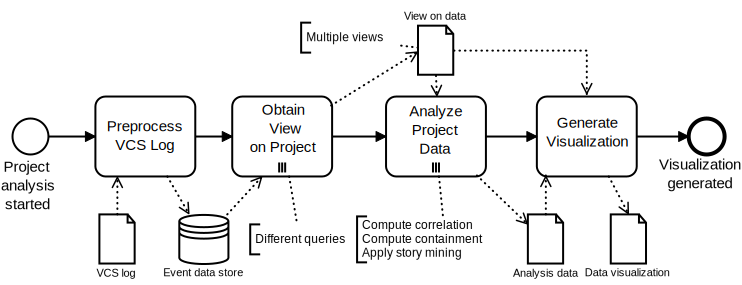
\includegraphics[width=.8\textwidth]{figures/visualization-process}
\caption[Generation of a process visualization from VCS logs]{Generation of a process visualization from VCS logs}
\label{fig:visualization-process}
\end{figure}

The first step of the approach is the preprocessing of the \gls{vcs} log received as input. The main goal of this phase is generate a set of events and store them into a database. Second, we obtain different views on the stored events. In particular, we are interested in observing
\begin{inparaenum}[\itshape i)]
	\item all the commits that affected the files over time;
	\item the amount of change brought by the commits to the files; and
	\item the users who issued such commits.
\end{inparaenum}
The third phase is responsible for considering the different perspectives defined by the project manager and through the generated views extract the necessary knowledge. The last phase is responsible for providing the visualization combining the different perspectives considered. In the following, we detail the formal concepts and the algorithm of our technique.

%\subsubsection{Preprocessing VCS Logs.}
%Version control system logs hold rich information about the artifacts and their evolution. Therefore, our process starts by extracting the elements \emph{Artifact}, \emph{Commit} and \emph{Event} from the log.
%
%First, the tree file is analyzed so the \emph{Parent} relation is defined. For that, the artifacts names appearing in the log are used. They provide the whole path from the root file until the leave file, which is the artifact in question. Thus, a parser can analyses the path and create the relation between the files. For instance, suppose we have the artifact \texttt{running example/software/model.java}. Three files are observed from this name: $f_1 = running \quad example$, $f_2 = software$ and $f_3 = model.java$. The following pairs will be included in the \emph{Parent} relation $\{(f_1,f_2),(f_2,f_3)\}$. 
%%are in the same containment if they share a common prefix that is maximal, i.e. they differ only by the name. For example, the files 
%%and \texttt{running example/software/test.java} . belong to the same containment, whereas the files  \texttt{running example/software/model.java} and \texttt{README.md} belong to two different containments. Note that containments can be contained in other containments, therefore every two files with eventually belong to the same containment. 
%
%Second, artifacts are extracted, as specified in Definition \ref{def_artifact}. Then the commits, following Definition \ref{def_commit}, are extracted. At last, the VCS raw log is transformed into a list of events for the extracted artifacts and commits, as specified in Definition \ref{def_event}. This step is easily done by replicating the information on commit level to be contained in the events. The amount of change is determined analyzing the attribute Diff of the VCS log. For instance, commit ID 2 in Table \ref{tab:vcs-log-data} indicates a commit with amount of change equals 3. The output of this phase is a set of events $E$, a set of artifacts $A$ and a set of commits $Com$.
%
%\subsubsection{Obtain View on Project.}
%The main goal of this phase is to extract the data that will be analyzed. The focus of this paper is in the artifacts, therefore the views generated gather information about events related to artifacts.  
%
%The project manager must determine the level of detail for the analyzes, thus, specifying the time windows. Input parameters of this phase are the interval of analysis ($ia$) and the time window for aggregation ($tw_{agg}$). Considering the specified $tw_{agg}$, the events generated in the previous phase are aggregated. For each artifact in a particular aggregate time an \emph{Aggregate Event} is generated as defined in Definition \ref{def_aggregateEvent}.
%
%\subsubsection{Analyze project data.}
%In this phase, the project is analyzed considering the different perspectives the project manager is interested in. In this paper, we considered three perspectives: dependency between artifacts, containments and artifact evolution.
%
%\paragraph{Dependency.} As stated in \Cref{def_dependency}, a dependency between two artifacts exists if both artifacts require a similar effort to be maintained, i.e. if they have a similar behavior considering the amount of changes.  The amount of change of an artifact over time defines  a time series. Therefore, for each artifact its aggregate events are analyzed in order to extract the amount of change for each aggregated time towards defining a time series for this artifact. 
%
%Let $AE$ be the set of aggregate events within $ia$. We build the time series for the \emph{i}-th artifact, namely $X_{f_i} = \lbrace (t, c) ~|~ e_a \in AE,~ t = ats(e_a),~ c = aac(e_a),~ f(e_a) = {f_i} \rbrace $. 
%
%%\todo[inline]{
%%Dependencies are obtained from the aggregated events. Considering the time window $tw$ and the aggregated event set in that time window ($AE_{tw}$), %$AE' = \lbrace e~|~ e \in AE,~ ts(e) \in tw \rbrace$,
%%we build the time series for the \emph{i}-th artifact, namely $X_{f_i} = \lbrace (t, c) ~|~ e_a \in AE_{tw},~ t = ats(e_a),~ t \in tw,~ c = aac(e_a),~ f(e_a) = {f_i} \rbrace $. As a result, the dependency between \emph{i}-th and the \emph{j}-th artifact is the correlation across time series $\sigma(i,j) = {corr(X_i, X_j)}$.
%%}
%
%After the time serie for each artifact is defined, the correlation function is used to calculate the correlation between the two time series. Considering artifacts $f_i$ and $f_j$ and the time series correspondent $X_{f_i}$ and $X_{f_j}$, $\sigma(f_i,f_j) = {corr(X_{f_i}, X_{f_j})}$ is the correlation value found when applying correlation function $corr$.
%
%If $\sigma(f_i,f_j)$ overcomes a threshold defined by the project manager (input parameter of this phase), then a dependency between the correspondent artifacts is established. The strength of the dependency is defined by $\sigma(f_i,f_j)$. 
%
%\paragraph{Containments.}
%For the containments extraction, the $Parent$ relation is analyzed and the set $C$ of containments defined.
%Containments reflect the hierarchical nature of the file structure in a repository. That is, \emph{composite containments} can be recursively decomposed into smaller containments until an \emph{atomic containment} is reached, following the tree structure of the file system top down. Conversely, from navigating the file structure bottom up, containments can be part of other containments until the root containment is reached. 
%
%
%\paragraph{Artifact evolution.}
%%For the artifact evolution definition, we propose to apply story mining techniques as follows.
%
%\input{sections/file-mining}

 %\hfill\\
%1. Compute correlation - dependency
%2. Compute containments 
%3. Apply story mining to obtain the process  - artifact evolution \\\hfill

%\subsubsection{Generate visualization.}
%%The approach is flexible making possible to generate different visualizations 
%In this section, we define the graphical elements of the visualization and their semantic. 
%
%%\input{table/visual-symbols}
%\paragraph{Project Participant.}
%%\todo[inline]{Task was not defined before. I think in our case workload will be in how many changes the project participant is involved within a period of time. I change to this idea. See what do you think. \\[2pt] I also consider project participant instead of resource following what was defined in section II.A. But I am ok with both. We just need to decide and change the whole paper. \\[2pt] The symbols have different faces and the semantic was not provided. I know they align with the color, but I think it is better to have the same face (not all people with high workload are sad or with low workload are happy). On the other hand, we lost the representation of a participant in the process, i.e. we are not able to visualize how many different participant worked in the same process (artifact). If we are still interested in that, I suggest to leave the faces as symbolizing the workload and the colors to symbolize different participants}
%
%Project Participants are displayed through a face symbol with its identification in the top, as depicted in  \Cref{fig:resources}. We use a color code to denote their level of workload, i.e. in how many changes the project participant is involved in the project within $ia$. \emph{Red}, \emph{yellow} and \emph{green} color indicate \emph{high}, \emph{medium} and \emph{low} project workload respectively. The project workload for a project participant ($wl_u$) is computed from the set of events in which the project participant was responsible for the change within $ia$, i.e. $wl_u(t_1,t_2) = |\lbrace e \in E ~|~  u(e)= u, t_1 \leq ts(e) \leq t_2 \rbrace|$, where $ia=[t_1 , t_2]$. These interval of analysis can be fine tuned to visualize the project participant occupancy over time. 
%
%%\begin{figure}[h]
%%	\centering
%%	\begin{subfigure}{.3\linewidth}
%%		\centering
%%		\begin{tikzpicture}[scale=.2]
%%		\node[text width=3cm] at (2,2.3) {resource};
%%		
%%		\filldraw [color=black, fill=green!50] (0,0) circle (2);
%%		\filldraw [color=black, fill=white] (-0.5,.6) ellipse (0.2 and 0.6);
%%		\filldraw [color=black, fill=white] (0.5,.6) ellipse (0.2 and 0.6);
%%		\filldraw [color=black, fill=black] (-0.5,.4) ellipse (0.2 and 0.3);
%%		\filldraw [color=black, fill=black] (0.5,.4) ellipse (0.2 and 0.3);
%%		\draw  (-1,-0.5) .. controls (-0.5,-1) and (0.5,-1) .. (1,-0.5);
%%		\draw  (-1,-0.5) .. controls (-0.5,-1.3) and (0.5,-1.3) .. (1,-0.5);
%%		\fill[fill=white, draw=black, opacity=1] (-1,-0.5) .. controls (-0.5,-1) and (0.5,-1) .. (1,-0.5) .. controls (0.5,-1.3) and (-0.5,-1.3) .. (-1,-0.5) --cycle;
%%		\end{tikzpicture}
%%		%		
\includegraphics[width=.3\linewidth]{figures/visualization-elements/green-face}
%%		\caption{}
%%		\label{fig:green}
%%	\end{subfigure}%
%%	\begin{subfigure}{.3\linewidth}
%%		\centering
%%		%		
\includegraphics[width=.3\linewidth]{figures/visualization-elements/yellow-face}
%%		\begin{tikzpicture}[scale=.2]
%%		\filldraw [color=black, fill=yellow!50] (0,0) circle (2);
%%		\filldraw [color=black, fill=white] (-0.5,.6) ellipse (0.2 and 0.6);
%%		\filldraw [color=black, fill=white] (0.5,.6) ellipse (0.2 and 0.6);
%%		\filldraw [color=black, fill=black] (-0.5,.4) ellipse (0.2 and 0.3);
%%		\filldraw [color=black, fill=black] (0.5,.4) ellipse (0.2 and 0.3);
%%		%mouth
%%		%		\draw  (-1,-0.6) .. controls (-0.5,-1) and (0.5,-1) .. (1,-0.5);
%%		%	\draw  (-1,-0.5) .. controls (-0.5,-1.3) and (0.5,-1.3) .. (1,-0.5);
%%		\fill[fill=white, draw=black, opacity=1] (-1,-0.7) .. controls (-0.5,-0.8) and (0.5,-0.8) .. (1,-0.7) .. controls (0.5,-1) and (-0.5,-1) .. (-1,-0.7) --cycle;
%%		\end{tikzpicture}
%%		\caption{}
%%		\label{fig:yellow}
%%	\end{subfigure}%
%%	\begin{subfigure}{.3\linewidth}
%%		\centering
%%		%		\includegraphics[width=.3\linewidth]{figures/visualization-elements/red-face}
%%		\begin{tikzpicture}[scale=.2]
%%		\filldraw [color=black, fill=red!60] (0,0) circle (2);
%%		\filldraw [color=black, fill=white] (-0.5,.6) ellipse (0.2 and 0.6);
%%		\filldraw [color=black, fill=white] (0.5,.6) ellipse (0.2 and 0.6);
%%		\filldraw [color=black, fill=black] (-0.5,.4) ellipse (0.2 and 0.3);
%%		\filldraw [color=black, fill=black] (0.5,.4) ellipse (0.2 and 0.3);
%%		%			\draw  (-1,-0.5) .. controls (-0.5,-1) and (0.5,-1) .. (1,-0.5);
%%		%		\draw  (-1,-0.5) .. controls (-0.5,-1.3) and (0.5,-1.3) .. (1,-0.5);
%%		\fill[fill=white, draw=black, opacity=1] (-1,-1) .. controls (-0.5,-0.5) and (0.5,-0.5) .. (1,-1) .. controls (0.5,-0.8) and (-0.5,-0.8) .. (-1,-1) --cycle;
%%		\end{tikzpicture}
%%		\caption{}
%%		\label{fig:red}
%%	\end{subfigure}
%%	\caption{Project Participant symbols. Color codes represent the status of their workload within a period of time.}
%%	\label{fig:resources}
%%\end{figure}
%
%
%%\begin{figure}[h]
%%	\centering
%%		\begin{tikzpicture}[scale=.2]
%%		\node[] at (0,3.5) {\textit{participant}};
%%		\filldraw [color=black, fill=white!50] (0,0) circle (2);
%%		\filldraw [color=black, fill=white] (-0.5,.6) ellipse (0.2 and 0.6);
%%		\filldraw [color=black, fill=white] (0.5,.6) ellipse (0.2 and 0.6);
%%		\filldraw [color=black, fill=black] (-0.5,.4) ellipse (0.2 and 0.3);
%%		\filldraw [color=black, fill=black] (0.5,.4) ellipse (0.2 and 0.3);
%%		%mouth
%%		%		\draw  (-1,-0.6) .. controls (-0.5,-1) and (0.5,-1) .. (1,-0.5);
%%		%	\draw  (-1,-0.5) .. controls (-0.5,-1.3) and (0.5,-1.3) .. (1,-0.5);
%%		\fill[fill=white, draw=black, opacity=1] (-1,-0.7) .. controls (-0.5,-0.8) and (0.5,-0.8) .. (1,-0.7) .. controls (0.5,-1) and (-0.5,-1) .. (-1,-0.7) --cycle;
%%		\end{tikzpicture}
%%	\caption{Project Participant symbol. The workload within a period of time is color coded.} 
%%	\label{fig:resources}
%%\end{figure}
%
%
%
%\paragraph{Dependency.}
%A dependency between two artifacts is represented by a line that connects their atomic containments. We label dependencies with a number  $\sigma \in \Re$, which indicates the strength of the dependency among the two artifacts. \Cref{fig:dependency} illustrate the notation for dependencies.
%
%%\begin{figure}[h]
%%	\centering
%%	%	\includegraphics[width=0.7\linewidth]{figures/visualization-elements/dependency}
%%	\begin{tikzpicture}[scale=.5]
%%	\draw[thick] (-2,0) -- node[above,thick] {$\sigma$} ++(4,0);
%%	\end{tikzpicture}
%%	\caption{Dependency with strength $\sigma$}
%%	\label{fig:dependency}
%%\end{figure}
%
%\paragraph{Artifact evolution.}
%
%The artifact evolution is a process under which the artifact changes step by step towards a final state reached eventually in the project (e.g. a documentation file reaches his final state when the documentation is complete and no edits are made to that version of document anymore). Thus, we chose the \gls{bpmn} to represent this process. 
%
%\Cref{fig:process} depicts an example of a process learned considering a story with two aggregated comments, thus a process with two sequential activities \emph{a} and \emph{b}, modeled in \gls{bpmn}. 
%
%%\tikzstyle{startstop} = [rectangle, rounded corners, minimum width=1.5cm, minimum height=1cm,text centered, draw=black, fill=white!30]
%%\tikzstyle{arrow} = [thick,->,-latex]
%%\tikzstyle{event} = [circle,scale=.5, minimum width=1cm, minimum height=1cm,draw,fill=white]
%%\tikzstyle{end event} = [event,ultra thick]
%%
%%\begin{figure}[h]
%%	\centering
%%	%
\includegraphics[width=0.7\linewidth]{figures/visualization-elements/process}
%%	\begin{tikzpicture}[scale=.3]
%%	\begin{scope}[auto, every node/.style={draw,circle},node distance=.2cm]
%%	\node (start) [event] {};
%%	\node (add) [startstop, right of=start, xshift=1.3cm] {a};
%%	\node (fix) [startstop, right of=add, xshift=1.9cm] {b};
%%	\node (end) [end event, right of=fix, xshift=2.8cm] {};
%%	\draw [arrow]  (start) -- (add);
%%	\draw [arrow]  (add) -- (fix);
%%	\draw [arrow]  (fix) -- (end);
%%	\end{scope}
%%	\end{tikzpicture}
%%	\caption{Process representing an artifact evolution using \gls{bpmn}.}
%%	\label{fig:process}
%%\end{figure}
%
%
%\paragraph{Containment.} 
%A containment is represented with a rectangle. 
%We overload the semantic of rectangle used to represent the containment with a time concept. The position of the \emph{atomic containments} is shifted within the boundaries of their parent containments according to the first timestamp of the artifact history. For example, given two \emph{atomic containments} $C_1\{f_i\}$, $C_2\{f_j\} \subseteq C$, and let $AE_i, AE_j \subseteq AE$ be the sets of aggregated events that affected these artifacts, respectively. Then $C_1$ is shifted left with respect to $C_2$ if $min\{ats(e) | e \in AE_i\} < min\{ats(e') | e' \in AE_j\}$. \Cref{fig:containment} illustrates this example.
%
%%\begin{figure}[h]
%%\centering
%%%\includegraphics[width=0.7\linewidth]{figures/visualization-elements/containment}
%%\usetikzlibrary{
%%	shapes.geometric,
%%	positioning,
%%	fit,
%%	calc
%%}
%%\begin{tikzpicture}
%%	\draw[thick] (0,0)rectangle (4,2) node[pos=.85] {$C_3$};
%%	\draw[thick] (1.1,1.1) rectangle (2.2,1.6) node[midway] {$C_1$}; 
%%	\draw[thick] (2.1,0.1) rectangle (3.2,0.6) node[midway] {$C_2$};
%%\end{tikzpicture}
%%\caption{A containment $C_3$ composed of two atomic containments $C_1$, $C_2$. $C_1$ is shifted more left wrt $C_2$ as its contained artifacts were affected by changes earlier.}
%%\label{fig:containment}
%%\end{figure}
%
%\begin{figure}
%	\centering
%	\begin{subfigure}[t]{.5\textwidth}
%		\centering
%		\begin{tikzpicture}[scale=.2]
%		\node[] at (0,3.5) {\textit{participant}};
%		\filldraw [color=black, fill=white!50] (0,0) circle (2);
%		\filldraw [color=black, fill=white] (-0.5,.6) ellipse (0.2 and 0.6);
%		\filldraw [color=black, fill=white] (0.5,.6) ellipse (0.2 and 0.6);
%		\filldraw [color=black, fill=black] (-0.5,.4) ellipse (0.2 and 0.3);
%		\filldraw [color=black, fill=black] (0.5,.4) ellipse (0.2 and 0.3);
%		%mouth
%		%		\draw  (-1,-0.6) .. controls (-0.5,-1) and (0.5,-1) .. (1,-0.5);
%		%	\draw  (-1,-0.5) .. controls (-0.5,-1.3) and (0.5,-1.3) .. (1,-0.5);
%		\fill[fill=white, draw=black, opacity=1] (-1,-0.7) .. controls (-0.5,-0.8) and (0.5,-0.8) .. (1,-0.7) .. controls (0.5,-1) and (-0.5,-1) .. (-1,-0.7) --cycle;
%		\end{tikzpicture}
%		\caption{Project Participant symbol. The workload within a period of time is color coded.} 
%		\label{fig:resources}
%	\end{subfigure}~
%	\begin{subfigure}[t]{.5\textwidth}
%		\centering
%		%	\includegraphics[width=0.7\linewidth]{figures/visualization-elements/dependency}
%		\begin{tikzpicture}[scale=.5]
%		\draw[thick] (-2,0) -- node[above,thick] {$\sigma$} ++(4,0);
%		\end{tikzpicture}
%		\caption{Dependency with strength $\sigma$}
%		\label{fig:dependency}
%	\end{subfigure}\\
%	\begin{subfigure}[t]{.5\textwidth}
%		\tikzstyle{startstop} = [rectangle, rounded corners, minimum width=1.1cm, minimum height=.6cm,text centered, draw=black, fill=white!30]
%		\tikzstyle{arrow} = [thick,->,-latex]
%		\tikzstyle{event} = [circle,scale=.7, minimum width=.5cm, minimum height=.5cm,draw,fill=white]
%		\tikzstyle{end event} = [event,ultra thick]
%		%		\begin{figure}[h]
%		\centering
%		%
\includegraphics[width=0.7\linewidth]{figures/visualization-elements/process}
%		\begin{tikzpicture}
%		\begin{scope}[auto, every node/.style={draw,circle},node distance=.05cm]
%		\node (start) [event] {};
%		\node (add) [startstop, right of=start, xshift=1cm] {a};
%		\node (fix) [startstop, right of=add, xshift=1.5cm] {b};
%		\node (end) [end event, right of=fix, xshift=1.6cm] {};
%		\draw [arrow]  (start) -- (add);
%		\draw [arrow]  (add) -- (fix);
%		\draw [arrow]  (fix) -- (end);
%		\end{scope}
%		\end{tikzpicture}
%		\caption{Process representing an artifact evolution using \gls{bpmn}.}
%		\label{fig:process}
%		%		\end{figure}
%	\end{subfigure}~~
%	\begin{subfigure}[t]{.45\textwidth}
%		\centering
%		%\includegraphics[width=0.7\linewidth]{figures/visualization-elements/containment}
%		\usetikzlibrary{
%			shapes.geometric,
%			positioning,
%			fit,
%			calc
%		}
%		\begin{tikzpicture}[scale=.99]
%		\draw[thick] (0,0)rectangle (4,2) node[pos=.85] {$C_3$};
%		\draw[thick] (1.1,1.1) rectangle (2.2,1.6) node[midway] {$C_1$}; 
%		\draw[thick] (2.1,0.1) rectangle (3.2,0.6) node[midway] {$C_2$};
%		\end{tikzpicture}
%		\caption{A containment $C_3$ composed of two atomic containments $C_1$, $C_2$. $C_1$ is shifted more left wrt $C_2$ as its contained artifacts were affected by changes earlier.}
%		\label{fig:containment}
%	\end{subfigure}
%	\caption{Graphic elements used to represent the defined concepts of project participant, work dependency, artifact evolution and containment.}
%\end{figure}
%
%\paragraph{Composing the visualization.}
%
%The layout rules to compose the visualization are the following. 
%\begin{inparaenum}[\itshape (i)]
%	\item Every element is within a containment, excluding the root;
%	\item Project participants responsible for the change are placed over \gls{bpmn} activities;
%	\item Artifact evolution is within an atomic containment;
%	\item Dependencies connect atomic containments, showing the strength of correlations between the belonging artifacts evolutions.
%\end{inparaenum}
%\Cref{fig:all-elements-together} shows the correct composition of the presented visual elements.
%
%\begin{figure}
%\centering
%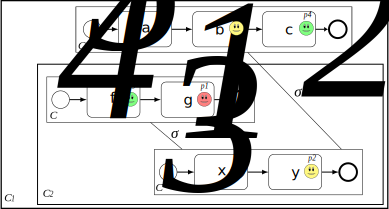
\includegraphics[width=.6\linewidth]{figures/visualization-elements/al-elements-together}
%\caption{Composition of the graphic elements into five containments, of which two are composite.}
%\label{fig:all-elements-together}
%\end{figure}



\subsection{Preliminaries}
\label{subsec:prelim}

%1. How we define/capture software processes\\

%2. How we define containment\\

%3. How we define dependencies\\

%Version control systems (VCSs) are used in projects to ensure reliable collaboration. We build our technique on \gls{vcs}. Typically, people work in VCS on files (e.g., text, source code, spread sheets) and commit them to the central repository. Project participants comment on their commits so that other participants can better understand the nature of the changes performed to the files.

As the objective of our technique is to uncover hidden work dependencies, we define the fundamental concepts required to capture them. Work is reflected by \emph{artifacts}, e.g., word documents, spreadsheets, code, etc. Artifacts are leaves in the file tree hierarchy (with directories being special type of non-leaf files). %Each directory in the file system groups together one or more files into a so-called \emph{containment}. 
Artifacts evolve over time, while project participants contribute their changes. Each change is an \emph{event} that happens to an artifact in a single point in time. Events can be abstracted into \emph{aggregated events} that allow a coarser grained view on the history. The history of the changes of an artifact over a time interval at a given level of abstraction is referred to as \emph{artifact evolution}. Similar artifact co-evolution establishes a \emph{dependency} between two artifacts. %In the following, we formally define the aforementioned concepts.

A software product is subdivided into files and directories. In this work, we consider directories as special type of files which are parents of other files. Formally, let $F$ be the universe of files in a software development project. Files are organized in a file tree. Therefore, each file $f \in F$ has one parent file. The only file without a parent file is the \emph{root} file. We capture this information in the parent relation $Parent: F \times F$. For example, let $f_p \in F$ be the parent of file $f_c \in F$, then $(f_p, f_c) \in Parent$. %Every file in $Parent$ defines a so-called \emph{containment}. For example, let $Parent = \{(f_{p_1} , f_{c_1})$, $(f_{p_1},f_{c_2})$, $(f_{p_2},f_{c_3})$, $(f_{p_3},f_{p_1})$,$(f_{p_3},f_{p_2})\}$, then files $f_{p_1}$, $f_{p_2}$ and $f_{p_3}$ define containments. Let $C$ be the set of containments. In our example $C=\{f_{p_1}, f_{p_2}, f_{p_3}\}$.
An \emph{artifact} is a file that is not a parent file, i.e. a file $f_a$ is an artifact if $\forall_{f \in F} (f_a, f) \notin Parent$.

%In this work, we are interested in describing the work progress related to a specific file, that we henceforth call \emph{artifact} and describe as follows:

%\begin{definition}
%	\label{def_artifact}
%	{\bf (Artifact)} An \emph{artifact} is a file that it is not a parent file, i.e. a file $f_a$ is an artifact if $\forall_{f \in F} (f_a, f) \notin Parent$.
%\end{definition}
%
%The files are grouped considering their organization in the tree file. We call each of these groups \emph{containments} and they are defined as follows:
%\begin{definition}
%\label{def_containment}
%{\bf (Containment)} A \emph{containment} is a file that is a parent of at least one other file. For example, let $Parent = \{(f_{p_1} , f_{c_1})$, $(f_{p_1},f_{c_2})$, $(f_{p_2},f_{c_3})$, $(f_{p_3},f_{p_1})$,$(f_{p_3},f_{p_2})\}$, then files $f_{p_1}$, $f_{p_2}$ and $f_{p_3}$ are containments. Let $C$ be the set of containments. In our example $C=\{f_{p_1}, f_{p_2}, f_{p_3}\}$.
%\end{definition}

%\begin{definition}
%	\label{def_artifact}
%	{\bf (File Containment)} An \emph{artifact} is a file that it is not a parent file, i.e. a file $f_a$ is an artifact if $\forall_{f \in F} (f_a, f) \notin Parent$.
%\end{definition}


%Containments can be either \emph{atomic} or \emph{composite}. An \emph{atomic containment} is a file which is parent of artifacts. In our example, containments $f_{p_1}$ and  $f_{p_2}$ are atomic containments.
%%\Cref{fig:containment} shows the visual symbol for an atomic containment.
%A \emph{composite containment} is a containment which is not atomic, i.e. it involves files which are parents of parents. In our example, containment $f_{p_3}$ is a \emph{composite containment}.  Therefore, the set $C$ of containments is partitioned in two subsets $C=C_1 \cup C_2$. In our example, $C=\{\{f_{p_1}, f_{p_2}\},\{f_{p_3}\}\}$.


% are defined, $C_1 = \{f_{c_1},f_{c_2}\}$ and $C_2=\{f_{c_3}\}$. A \emph{containment} $C$ is a set of files with the same parent file. For example, let $Parent = \{(f_{p_1} , f_{c_1}), (f_{p_1},f_{c_2}), (f_{p_2},f_{c_3})\}$, then two containments are defined, $C_1 = \{f_{c_1},f_{c_2}\}$ and $C_2=\{f_{c_3}\}$.

When project participants do a certain amount of work and want to save their current progress, they commit the changes to the \gls{vcs}. We define changes on artifacts as the \emph{events} of interest on the lowest granularity.

\begin{definition} {\bf(Event)}
\label{def_event}
Let $E$ be the set of events. An \emph{event} $e \in E$ is a five-tuple $(f, ac, ts, k,u)$, where
\begin{itemize}
\item $f \in F$ is the affected artifact of the event.
%\item $o \in O$ = \{added, modified, deleted\} is the change operation on the artifact with obvious meaning.
\item $ac \in AC =  \mathbb{N}$ is the amount of change done in the artifact.
\item $ts \in TS = \mathbb{N}$ represents a unix time stamp marking the time of the event occurrence.
\item $k \in \Sigma ^* $ is a comment in natural language text.
\item $u \in U$ is the project participant responsible for the change.
\end{itemize}
\end{definition}

For event $e = (f, ac, ts, k,u)$ we overload $f$, $ac$, $ts$, $k$ and $u$ to be used as accessor functions. For example, $f$ is the function $f : E \rightarrow F$ mapping an event to its affected artifact.

In some situations, it can be interesting to have a higher level overview of the changes done to a particular artifact. In this case, an aggregation of events related to this artifact in an interval of time can be performed. The time window for the aggregation, henceforth denoted as $tw_{agg}$, must be defined, i.e. the size of the time interval. For instance, a time window for aggregation can be a day. Thus, all events occurring for an artifact in the same day will be aggregated. An \emph{aggregated event} is defined as follows:

\begin{definition} {\bf (Aggregated Event)}
\label{def_aggregateEvent}
An \emph{Aggregated Event} for $tw_{agg}$ ($AE_{tw_{agg}}$) is a five-tuple $(f, aac, ats, ak,au)$, where
\begin{itemize}
\item $f \in F$ is the affected artifact in the set of events being aggregated.
%\item $ao \in O$ = \{added, modified, deleted\} is the aggregated change operation on the artifact. If the only change operation performed in $tw_{agg}$ was \emph{added} or \emph{deleted} then the aggregated change operation is the same, otherwise it is \emph{modified}.
\item $aac \in AAC =  \mathbb{N}$ is the aggregate amount of change done in the artifact for $tw_{agg}$. It is calculated by summing the amount of changes done in each of the time aggregated.
\item $ats \in ATS = \mathbb{N}$ represents an aggregate time of the unix time stamp of the events being aggregated.
\item $ak \in \Sigma ^* $ is the concatenation of the comments presented in the events being aggregated.
\item $au \subseteq U$ are the project participants responsible for the changes in $tw_{agg}$ being aggregated.
\end{itemize}
\end{definition}
%\todo[inline]{We consider a $tw$ but do not use it in the definition.}

The set of aggregated events for a particular artifact defines how this artifact evolves over time. Considering an interval of analysis, henceforth denoted as $ia$, we define artifact evolution as follows.

\begin{definition} {\bf (Artifact Evolution)}
%Let $EA_f$ be the set of all aggregated events related to artifact $f$.
\emph{Artifact evolution} is the process describing how the file $f$ changed over an interval of time $ia$, i.e., a set of labeled tuples $A_{evo}(f) = \{ (t,a,l) | e \in AE_{ia}, f=f(e), t=ats(e), a=aac, l=ak(e)\}$ chronologically ordered.

%The comments associated to the aggregated events in $EA_f$ define the activities executed. The time of the aggregated events in $EA_f$ establishes the order of the activities and then the flow of evolution. Each activity is associated with the user that executed it.
\end{definition}

%Project participants can commit a number of changes to different artifacts at one step. Therefore, we define the notion of commits as follows.
%
%\begin{definition} {\bf (Commit)}
%\label{def_commit}
%A \emph{commit} $Com$ is a set of events sharing the same time stamp and comment, i.e., $\forall e, e'\in Com : ts(e) = ts(e')\wedge k(e) = k(e')$. Additionally, each event in a commit affects different artifact, i.e., $\forall e, e' \in Com : e \neq e' \rightarrow f(e) \neq f(e')$.
%\end{definition}

%For example, a dependency is established if the two artifacts require a similar effort to be maintained. The effort of maintenance is measured through the amount of changes done to the artifact.

%\begin{definition} {\bf (Dependency)}
%\label{def_dependency}
%A \emph{dependency} between two artifacts within $ia$ is a similarity function $\sigma : X_{evo} \times X_{evo} \rightarrow \mathbb{Z}$, where the artifact evolution set in which the labels are projected out, i.e $X_{evo} = \{(t,a) | \exists l : (t,a,l) \in A_{evo}\}$.
%%Thus, each artifact defines a time series of the amount of change. If the correlation between two time series is significant then a dependency between the correspondent artifacts is established. The strength of the dependency is defined by the correlation value.
%\end{definition}
%
%
%
%\subsection{Metrics} 

Note that artifact evolution represents the changes that happened to a file over time. Thus, we can build the time series of a file $f$ as the vectors of changes $\vec{X_{f}} = (a_1, ..., a_n)$ in the time window $tw_{agg} = [t_1,t_n]$, with $a_i$ being the sum of the changes of $f$ in of the aggregated intervals $t_i$ of the time window $tw_{agg}$.

%The file system establishes a structural tree-based relationship among files. However, other types of dependencies can emerge between two files. In this paper, we define dependency between two files in terms of their \emph{degree of co-evolution}.
%In this paper, we are interested in measuring the hidden work-dependencies among artifacts of the project-oriented business process. That is, we want to capture dependencies that are created among files that go beyond functional (e.g. interface-implementing class) or structural (e.g., parent-child in the file tree structure).

%We define the metrics of \emph{degree of co-evolution} and \emph{file distance}. 

We measure the dependency between two files $f_a$ and $f_b$ in terms of their \emph{degree of co-evolution} as follows.
\begin{definition} {\bf (Degree of Co-Evolution)} 
	\label{definition:degree-of-coevolution}
	Given two files $f_a$ and $f_b$, the \emph{degree of co-evolution} $\chi: F \times F \rightarrow [0,1]$ is a similarity function of the respective time series.
\end{definition}
In this paper, we fix $\chi(f_a,f_b) = |\sigma (\vec{X_{f_a}}, \vec{X_{f_b}})|$, where $\sigma$ is the correlation function of the two vectors $\vec{X_{f_a}}$ and $ \vec{X_{f_b}}$.

The way files are kept in the directory structure establishes an inherent relationship among files being stored close to each other in the hierarchy. For instance, files serving the same purpose are stored close to each other in the file system. 
Hidden work dependencies are expected to happen between artifacts that are distant in the file structure. We measure this distance as the length of the shortest route connecting two files in the file tree. We adapt the notion of path from~\citep{Gubichev2010} to our file tree. Given a file $f$, the path to the root node can be obtained by navigating the $Parent$ relationship up to the root file. The path $p$ from $f_a$ to the root $f_r$ is the set of parent files encountered along such route. i.e. $p(f_1,f_{r}) = \{(f_1, ..., f_k, f_{k+1}, ..., f_{r})\}$ such that for any $k$, $(f_{k+1},f_k) \in Parent $. The length of the path is the cardinality $|p|$ of the set. 
The shortest path between two files $f_a$, $f_b$ in a tree passes through the \gls{lca}~\citep{Bender2000}. This is equivalent to considering the paths from the single files to the root node $p_a = p(f_a,f_r)$ and $p_b=p(f_b, f_r)$ minus their intersection $I_{p_a,p_b}=\{p(f_a, f_r) \cap p(f_b, f_r)\}$. Thus, we define the \emph{file distance} as the length of the shortest path between two files $f_a$ and $f_b$ as follows. 

\begin{definition} {\bf (File Distance)} 
	\label{definition:artifact-distance}
	The distance $d : F \times F \rightarrow \mathbb{N} $ between two files belonging to the same directory structure is defined as the number of nodes in the minimum path connecting the two files in the project file tree: $d(f_a,f_b) =  |p_a| + |p_b| - 2*(|I_{p_a,p_b}|)$.
\end{definition}
 

\subsection{Hidden Dependencies Discovery Algorithm}

We are focused on finding interesting hidden work dependencies. These dependencies are typically reflected by changes that happen to couples of allegedly unrelated files during their evolution. This section details the procedure that implements the technique outlined in \Cref{fig:visualization-process}.

\Cref{algorithm:all} presents the steps required to explicate such hidden dependencies. The procedure $\mathtt{PreprocessLog(\mathcal{L})}$ in line~\ref{step:preprocess} takes as input a VCS log $\mathcal{L}$ structured as in \Cref{tab:vcs-log-data} and parses out work events at the granularity of line changes. These events are then stored into an event data storage. Events parsed from \gls{vcs} logs contain rich information about multiple aspects of the work they reflect. In order to represent all these different aspects, we devised the entity-relationship data model. Hence, we are able to store all the information that is possible to obtain after parsing the \gls{vcs} log. Furthermore, this step allows the user to obtain simple information, such as statistics on the project, already at an early stage of the procedure. The output of the $\mathtt{PreprocessLog(\mathcal{L})}$ step results in the storage of all the events $E$ into a database.
%Further on, we will show a possible implementation that uses a database to store the parsed events, but in principle any type of repository that allows to store the preprocessed events can be considered.

%\begin{figure}
%	\centering
%	\includegraphics[width=.8\textwidth]{figures/CommitLogER3.pdf}
%	\caption{Entity-Relationship model used to store events extracted from VCS logs}
%	\label{fig:data-model}
%\end{figure}


Next, the iterative call of the procedure $\mathtt{RetrieveView(\mathit{E}, \mathsf{query})}$ in line \ref{step:retrieve-view} performs several querying the data storage containing the set $E$. For example, a possible query can obtain all the comments associated to each change of a specific file. To obtain information on the evolution of files, we query the database for the changes of all the files within a user defined time interval $tw_{agg}$. In general several time frames can be chosen, each of them producing a \emph{view} $V$ on the data, i.e., a set of aggregated events chronologically sorted within $tw_{agg}$. For example, users may be interested in artifact-views aggregated by day, by month, etc. Multiple \emph{views} are possible by defining them in the {\textsf{queries}} parameter. We collect these views into a set $\mathcal{V} = \bigcup_{\textsf{queries}} V$. 

%Step~\ref{step:contaiments} extracts the structural relationships among the file paths contained in each view $V$, i.e., it recreates the file tree from the artifacts.


\input{bpm2017/algorithms/all}%\input{algorithms/RetrieveView}
%\Cref{algorithm:compute-containments} computes the containments. Note that both atomic and composite containments are computed.

%\input{algorithms/ComputeContainments}

The step in line~\ref{step:evolution} starts an iteration over the views set $\mathcal{V}$. Here is where we collect the analysis data that are returned by the algorithm. For each of the aggregated artifacts contained in a view $V$, we retrieve the information necessary to compute the \emph{degree of co-evolution} between pairs of files and their \emph{file distance}. First, we construct the artifact evolution of all the artifacts present in $ae \in V$. 
Note that an aggregated event $ae \in V$ is a record obtained from a view on the project which is composed, among other attributes (e.g., file, time, amount of change), by the comment associated to the specific change. Comments describe multiple changes executed on the file, i.e. they describe a \emph{story} of the artifact. 
Stories associated to each file are collected and the corresponding labels are chronologically ordered. These file stories are then input to the StoryMining technique~\cite{Goncalves2011}. Story Mining was designed to receive as input a story freely written by the participants, describing their work in a particular business process. As an output, the \emph{actors} and the process \emph{activities} executed by them are extracted. Our technique is concerned with the stories of the files. Therefore, they are the actors of the story mining, and the resulting business process consists of the steps describing their evolution process. We collect the resulting processes in the step in line~\ref{step:story-mining}.
The step in line~\ref{step:timeseries} is concerned with the construction of a time series from the set of artifact evolutions $A_{evo}$ computed in line~\ref{step:a-evo}. Specifically, this step gathers the values of the changes of each of the artifact $f$ in $A_{evo}$ and records them in $TimeSeries(f)$. 

After all the aggregated events $ae$ have been explored, the algorithm moves on to computing the metrics (lines~\ref{step:metric-start}--\ref{step:metric-end}). In this loop, the algorithm iterates through all the pairs of files. For each pair, the \emph{degree of co-evolution} and \emph{artifact-distance}  metrics are computed according the \Cref{definition:degree-of-coevolution} and \Cref{definition:artifact-distance}, respectively. These two measures are collected only if their values are above the user defined thresholds $\gamma$ and $\delta$. After the loop is over, the two measurements and the stories mined with the StoryMiner are stored in $AnalysisData$.

Finally, after iterating over all the user defined views, the algorithm returns the $AnalysisData$ collection which can now be further inspected and analyzed in more detail, as we show next with an example.

%\input{algorithms/ComputeEvolution}



%\input{algorithms/ComputeDependencies}
%
%The algorithm iterates over the views and creates the time series from the aggregated events $v$ in each of the views $V$ of the view collections $\mathcal{V}$. A time series is captured by a set $X_{f_i}$, recording the trend of the changes of file $f_i$ over the time. Next, the dependencies are calculated by using the similarity function $\sigma$ (cf. \Cref{def_dependency}) pairwise over the time series of the different artifacts. We do not enforce a determined similarity function between time series. The user can adopt a customized time series similarity function or use an existing method from literature (e.g.~\cite{ruohonen2015time}). Because the time series must have equal length, we add missing times $t$ with couples $(t,0)$. These couples denote that the amount of change in $f$ at time $t$ was 0. Finally, we collect the results in the dependencies set $D$ if they are stronger than the threshold $\delta$.



%\input{sections/metrics}


%\subsection{Story Mining}
\label{subsec:story-mining}

%What is story mining and how we use it in our work
Gon\c{c}alves et al.~\cite{Goncalves2011} proposed a story mining approach to extract process elements from stories, i.e. text descriptions written collaboratively by the process participants. A story is a natural way to transmit and share knowledge. Using both natural language (text) and contextual elements (categorization of parts of the story), storytellers can express their experience and viewpoints about the work processes they participate, interact with and/or perceive. Stories have the advantage of reproducing the situations associated with their contexts - the knowledge that is difficult to capture in interviews or mining from Information Systems logs. Since collectively told, a story incorporates a range of perspectives. Business processes instances can also be viewed as stories played by individuals who perform specific roles depending on the circumstances.

Story Mining  \cite{Goncalves2011} receives as input a story freely written by the participants, describing their work in a particular business process. As an output, the \emph{actors} and the process \emph{activities} executed by them are extracted. To illustrate the approach consider the following story. The terms highlighted in {\bf bold} are the actors of the processes and the terms highlighted in {\color{gray} gray} the activities. 

\begin{figure}[!h]
{ \bf The system} {\color{gray} generates an estimating template consisting of the phases, activities and tasks} selected
for the project or project phase. When planning complete projects the estimating is typically done at the activity level, using the
list of tasks in the work breakdown as input to the estimating process. However {\bf estimators} will likely {\color{gray}add an itemized list of system functions and other deliverables}, to facilitate estimating the construction phase. {\bf Multiple estimators} {\color{gray} prepare estimates for each component}, {\color{gray}compare their estimates}, and {\color{gray}arrive at a final estimate} for each item.
  \label{RB}
\end{figure}

A further step that we developed in our approach is the identification of the relationship between the activities, therefore defining the flow.

%\subsection{Project Mining Software Projects}
\label{subsec:proj-mining}

Project mining technique 


\section{Evaluation}
\label{sec:evaluation}

In this section, we show the applicability of our technique to project-oriented business processes and its effectiveness in uncovering work dependencies. With respect to the requirements formulated in \Cref{sec:background}, we evaluate against requirements {R2} and {R3} in \Cref{subsec:quantitative-eval} and against requirement {R1} in \Cref{subsec:qualitative-eval}.

We implemented our techniques as a prototype\footnote{The source code is available at \url{https://github.com/s41m1r/MiningVCS}} and used it on 10 real world software projects with different sizes. The input of our program is a \gls{vcs} log and the output is a set of analysis data with information about the evolution of the artifacts and their dependencies. We report the results in \Cref{table:evaluation-results-new}. The results are listed in increasing order of project size. The parameters $\chi$ and $d$ are the metrics of \emph{degree of co-evolution} and \emph{distance}, respectively. In this example, $\chi > 0.7$ signifies that the co-evolution is high ($\chi^{H}$) and $\chi < 0.3$ that the co-evolution is low ($\chi^{L}$). As previously mentioned, this is a user customizable threshold that can be set by the domain expert. Likewise, the distance is considered low ($d^{L}$) when $d<=2$ and high ($d^{H}$) when $d>2$. The parameter  $\overline{|p_f|}$ and {$max(|p_{f}|)$} are respectively the average and the maximum lengths of the path to the root (i.e. average tree depth of the files). The column {$|A_{evo}|$} shows the average number of activities in the process representing the artifact evolution. Lastly, the columns {$\overline{d}$} and {$max(d)$} report the average and maximum file distance, respectively. Next, we use these data for a quantitative evaluation of the projects.

% Please add the following required packages to your document preamble:
% \usepackage{graphicx}
\begin{table}[t]
\centering
\caption[Evaluation on project metric on real world projects.]{Evaluation of real world projects. Respectively the thresholds are: $\chi^{L}$ if $\chi < 0.3$,  $\chi^{H}$ if $\chi > 0.7$  low and high degree of co-evolution; $d^{L}$ if $d \leq 2$,  $d^{H}$ if $d > 2$ respectively low and high distance.}
\label{table:evaluation-results-new}
\resizebox{\textwidth}{!}{%
\begin{tabular}{rrrrrrrrrrrrrr}
Project                 & \rot{Commits} & \rot{Files} & \rot{$\chi^{H}$} & \rot{$\chi^{L}$} & \begin{tabular}[b]{@{}r@{}}{\rot{$(d^{L},\chi^{L})$}}\end{tabular} & \begin{tabular}[b]{@{}r@{}}{\rot{$(d^{L},\chi^{H})$}}\end{tabular} & \begin{tabular}[b]{@{}r@{}}{\rot{$(d^{H},\chi^{L},)$}}\end{tabular} & \begin{tabular}[b]{@{}r@{}}{\rot{$(d^{H},\chi^{H})$}}\end{tabular} & \rot{$\overline{|p_f|}$} & \rot{$max(|p_{f}|)$} & \rot{$|A_{evo}|$} & \rot{$\overline{d}$} & \rot{$max(d)$} \\ \midrule
%smsr                    & 21        & 6         & 22                   & 6                  & 0                          & 9                            & 6                       & 13                        & 2.71             & 5             & 1.82                    & 1.43                & 6                  \\
mwaligner  & 21      & 9     & 37                   & 7                 & 6                               & 30                                 & 1                                          & 7                                             & 1.11              & 2           & 2.40         & 0.94                 & 3                 \\
Biglist                 & 202     & 15    & 22                   & 90                & 31                              & 18                                 & 59                                         & 4                                             & 1.47              & 3            & 2.76         & 1.20                 & 5                 \\
camundaRD & 11      & 15    & 74                   & 26                & 0                               & 25                                 & 26                                         & 49                                            & 2.18              & 4            & 2.05         & 2.03                 & 7                 \\
graphql                 & 256     & 30    & 89                   & 357               & 121                             & 89                                 & 236                                        & 0                                             & 1.40              & 2            & 3.18         & 1.11                 & 4                 \\
jgitcookbook            & 135     & 89    & 773                  & 2866              & 505                             & 289                                & 2361                                       & 484                                           & 6.93              & 8            & 1.33         & 2.68                 & 14                \\
mysqlpython             & 749     & 168   & 2288                 & 11571             & 742                             & 591                                & 10829                                      & 1697                                          & 2.59              & 7            & 1.65         & 2.52                 & 11                \\
gantt                   & 23      & 228   & 7006                 & 14343             & 386                             & 3480                               & 13957                                      & 3526                                          & 3.30              & 4            & 1.71         & 2.16                 & 7                 \\
facebookjavasdk         & 38      & 293   & 16478                & 26092             & 2017                            & 16311                              & 24075                                      & 167                                           & 6.21              & 8            & 4.78         & 5.58                 & 13                \\
caret                   & 864     & 432   & 15366                & 60874             & 9538                            & 14785                              & 51336                                      & 581                                           & 3.01              & 4            & 3.15         & 1.60                 & 7                 \\
operationcode           & 1114    & 1053  & 84024                & 444605            & 2291                            & 5537                               & 442314                                     & 78487                                         & 4.27              & 8            & 2.01         & 4.85                 & 15               \\ \bottomrule
\end{tabular}%
}
\end{table}
%\vspace*{1cm} 

%\subsection{Prototypical Implementation}
\label{subsec:prototype}


%
%The first step of the approach is the preprocess of the VCS log received as input. The main goal of this phase is generate a set of events and store them into a database. Second, we obtain different views on the stored events. In particular, we are interested in observing
%\begin{inparaenum}[\itshape i)]
%	\item all the commits that affected the files over time;
%	\item the amount of change brought by the commits to the files; and
%	\item the users who issued such commits.
%\end{inparaenum}
%The third phase is responsible for considering the different perspectives defined by the project manager and through the generated views extract the necessary knowledge. The last phase is responsible for providing the visualization combining the different perspectives considered. The following sections detail each of the phases.

We implemented our technique as a prototype\footnote{\url{https://github.com/s41m1r/MiningVCS.git}}. The input of our program is a \gls{vcs} log and the output is a set of analysis data with information about the evolution of the artifacts and their dependencies. 
%%Next we show the implementation details of \Cref{algorithm:all}.
%
%
%
%%\subsubsection{Preprocess VCS Logs.}
%As a first step (cf.~\Cref{algorithm:all}) we need to preprocess the input in order to extract events. Events in \gls{vcs} have multiple dimensions and relations among one another. Therefore, the natural way of capturing them is through a relational data model. This model serves at structuring the raw data and persisting the results after first step of \Cref{algorithm:all}. \Cref{fig:data-model} outlines the main entities in a \gls{vcs} and the relationships of our interest. The result the first step of \Cref{algorithm:all} is the correct population of the a database with the set of the extracted events, stored according to the relational schema. 
%
%\begin{figure}[]
%	\centering
%	\includegraphics[width=0.9\linewidth]{figures/CommitLogER}
%	\caption{Relational schema of a software project}
%	\label{fig:data-model}
%\end{figure}
%
%%\subsubsection{Obtain View on Project.}
%
%The step~\ref{algorithm:all} makes queries over the event set in order to retrieve aggregated views from them. This is simply done by defining queries on the database and export collect their results (e.g., in a CSV file). Step~\ref{step:contaiments} consists in recreating the file structure. This is implemented by reverse engineering the directory structure from the \texttt{path} attribute of the entity \texttt{File} that is present in the output of the query. Next, we actuate step~\ref{step:evolution} by implementing \Cref{algorithm:compute-evolution} that computes the artifact evolutions. This algorithm takes as input the set of views calculated previously and outputs \begin{inparaenum}[\itshape i)]
%	\item and a set of \emph{file stories} that report the amount of change, time and comments of the file history, and
%	\item a set process that describe the evolution of every artifact obtained by story mining~\cite{Goncalves2011} the file stories.
%\end{inparaenum} Finally, for step~\ref{step:dependencies} we implement \Cref{algorithm:compute-dependencies}. This algorithm takes as input the aggregated views obtained previously and two parameters: a comparison function and a threshold. We use the Pearson correlation $\rho$ and let the domain expert set the threshold $\delta$ to filter the strength of the dependencies. An important step before 


%One example of query that outputs a view of the daily changes of the artifact \texttt{model.java} is shown in \Cref{lst:query}. 

%\begin{center}
%\begin{lstlisting}[
%language=SQL,
%showspaces=false,
%float=ht,
%xleftmargin=4em,
%aboveskip=6pt,
%belowskip=0cm,
%belowcaptionskip=0cm,
%basicstyle=\ttfamily\scriptsize,
%showstringspaces=false,
%commentstyle=\color{gray},
%mathescape=true,
%caption={SQL query to obtain the artifact history for a given artifact, aggregated on a day level},captionpos=b, label={lst:query}
%]
%SELECT CONCAT(Commit.comment,$\S$) as Comments, 
%	DATE(Commit.timeStamp) as Date, 
%	sum(linesAdded+linesRemoved) as Change, 
%	CONCAT(User.name, '$\S$') as Users
%FROM File, Edit, acts,Commit,User 
%WHERE File.path = 'model.txt' 
%	AND Edit.commit_id = Commit.id 
%	AND Edit.file_path = File.path
%	AND User.id = Commit.user_id
%	AND acts.file_path = File.path 
%	AND acts.commit_id = Commit.id
%GROUP BY Date
%ORDER By Date ASC
%\end{lstlisting}
%\end{center}
%
%\Cref{table:analysis-data} depicts a view obtained with the query in \Cref{lst:query} on the project shown in \Cref{subsec:scenario}. The data is aggregated by day. String values are concatenated together with the symbol '$\S$'.
%
%\input{tables/analysis-data}

%\subsubsection{Analyze project data.}

%The input of this phase is a collection resulting from querying all the artifact histories from the data store. At this point the data is ready to be analyzed. 
%In this step analyses on the view extracted are performed. There are a number of different analyses that can be applied directly to the \emph{aggregate events}, e.g. checking whether project participants have been working on the assigned tasks ("Are they working in the artifacts they should/?") or there has rather been disorganization in regards. In this work, we focus on analyzes related to the artifacts, i.e. how they evolve over time, how they are organized and how are the dependencies among them. Therefore, in this section we focus on extracting the \emph{containments}, \emph{dependencies} and \emph{artifact evolution} elements.
%
%Analyzing the \emph{Parent} relation, the set $C$ of containments for our scenario of use is: $C = \{f_1, f_3, f_4, f_6, f_9, f_{10}\}$. 
%
%\begin{table}[t]
%%	\centering
%	\caption{Time series similarity among the six artifacts}
%	\label{table:time-series-all}
%	\begin{subtable}{.45\linewidth}
%		\input{tables/times-series}
%	\end{subtable}
%	\begin{subtable}{.45\linewidth}
%		\input{tables/correlations}
%	\end{subtable}
%\end{table}
%
%To compute the dependencies, we analyzed the time series depicted in \Cref{table:time-series} computing the correlations pairwise. Considering that the project manger specified a threshold of 0.7, we found the dependencies: \{(${f_7}$,${f_5}$), (${f_7}$,${f_8}$), (${f_2}$,${f_5}$), (${f_2}$,${f_{12}}$), (${f_5}$,${f_{12}}$)\}.
%
%The last step in this phase is the computation of the artifacts evolution. For all 6 artifacts a story containing the comments observed in the aggregate events for that artifact was generated. In the end, six stories were created and for each of them our approach for artifact mining was applied. 

\subsection{Quantitative Evaluation}
\label{subsec:quantitative-eval}

We implemented our techniques as a prototype\footnote{The source code is available at \url{https://github.com/s41m1r/MiningVCS}} and used it on 10 real world software projects with different sizes. The input of our program is a \gls{vcs} log and the output is a set of analysis data with information about the evolution of the artifacts and their dependencies. We report the results in \Cref{table:evaluation-results-new}. The results are listed in increasing order of project size. The parameters $\chi$ and $d$ are the metrics of \emph{degree of co-evolution} and \emph{distance}, respectively. In this example, $\chi > 0.7$ signifies that the co-evolution is high ($\chi^{H}$) and $\chi < 0.3$ that the co-evolution is low ($\chi^{L}$). As previously mentioned, this is a user customizable threshold that can be set by the domain expert. Likewise, the distance is considered low ($d^{L}$) when $d<=2$ and high ($d^{H}$) when $d>2$. The parameter  $\overline{|p_f|}$ and {$max(|p_{f}|)$} are respectively the average and the maximum lengths of the path to the root (i.e. average tree depth of the files). The column {$|A_{evo}|$} shows the average number of activities in the process representing the artifact evolution. Lastly, the columns {$\overline{d}$} and {$max(d)$} report the average and maximum file distance, respectively. Next, we use these data for a quantitative evaluation of the projects.

\input{bpm2017/tables/evaluation-table-new}


Next, we address requirements R2 and R3. First, we compute project profiles. These profiles show the distribution of work-related dependencies in a project. Second, we evaluate whether the work on files can be predicted.

Before assessing project profiles, we make the following consideration. Our metrics define four classes:
\begin{inparaenum}[\itshape i)]
	\item low distance low co-evolution;
	\item high distance low co-evolution;
	\item low distance high co-evolution;
	\item high distance high co-evolution.
\end{inparaenum} \Cref{fig:pairs-on-space} helps clarifying these four classes. In fact, except for values of distance equal to 0, it is possible to see how the density of file pairs is higher when the distance is low. This is a normal situation in project where highly related files are stored closely to each other in the file system. Conversely, the dots on the top right of the plot mark files which are very distant to each other but still highly correlated. These can be, for instance, logical dependencies that can happen because of bad modularization of the project.

Hidden work dependencies belong to the last mentioned case, i.e. files are distant in the file tree but they have similar time series. According to this consideration we computed the project profiles in \Cref{fig:project-analysis}. We observe three types of processes. First, several projects have hardly any hidden work dependencies. Second, several have a moderate degree between 10\% and 20\%. Third, the project \textit{Biglist} has a high share of hidden dependencies. This hints at the possibility for better organizing the project according to good modularization best practices. That means, the project can be restructured in a way to reduce the unwanted side-effect the work on one file produces on other files.
%\input{tables/project-assessment}


%\begin{figure}
%\centering
%
\includegraphics[width=0.3\linewidth]{figures/assessment-diagram}
%\caption{Project assessment diagram}
%\label{fig:assessment-diagram}
%\end{figure}
\begin{figure}[t]
	\begin{subfigure}[b]{.51\textwidth}
		\centering
		\includegraphics[width=.98\linewidth]{bpm2017/figures/Project-Analysis-Barchart-crop.pdf}
		\caption{Evaluation on real projects}
		\label{fig:project-analysis}
	\end{subfigure}~
	\begin{subfigure}[b]{.47\textwidth}
		\centering
		\includegraphics[width=.98\linewidth]{bpm2017/figures/Co-EvolutionVSDistance-OneColor.pdf}
		\caption{Distribution of pairs on real projects}
		\label{fig:pairs-on-space}
	\end{subfigure}
%	\vspace*{-.5cm}
	\caption{Characterization of the evaluated software projects}
\end{figure}
Next, we evaluate whether the work on files can be predicted. Zipf's law is typically used in corpus analysis and states that the \emph{frequency} of usage of any word is inversely proportional to its \emph{rank} in the frequency table. This approach has already been applied to software projects for understanding whether the assignment of developers to tasks in a software project could be predicted~\cite{Canfora2006}. Here, we focus on understanding whether the Zipf's law holds true also for work dependencies within a project. 

To this end, we selected one big and one small project from \Cref{table:evaluation-results-new}, namely \emph{Biglist} and \emph{Caret}. Biglist is a small project on a list of strings which are known to cause issues when used as user-input data. Caret is a big project consisting in the development of a sublime text editor for Chrome OS.
We collected how frequently were the artifacts worked on to generate a ranking. \Cref{fig:zipf-graph} depicts the corresponding charts and the fitted Zipf distribution. We notice that both projects present a similar distribution of values. This holds also for the other projects analyzed. In particular, Zipf's law is valid for the most frequently changed files. Afterwards, the distribution drops because of files not being worked anymore but still being part of the project.
%In pure software development projects, the tail can hint at some dead code and the need for maintenance.

\begin{figure}[t]
%	\centering
	\begin{subfigure}{.5\textwidth}
		\centering
		\includegraphics[width=\linewidth]{bpm2017/figures/biglist-new-crop}
		\caption{Biglist project}
		\label{fig:biglist}
	\end{subfigure}%
	\begin{subfigure}{.5\textwidth}
		\centering
		\includegraphics[width=\linewidth]{bpm2017/figures/caret-new-crop}
		\caption{Caret project}
		\label{fig:caret}
	\end{subfigure}
%	\vspace*{-.3cm}
	\caption{Zipf distribution of the worked files}
	\label{fig:zipf-graph}
\end{figure}
%\vspace*{-.2cm}

\section{Discussion}
\label{subsec:qualitative-eval}

In this section, we address requirement R1 by showing insights on the work history of files that are related. To this end we focused on the project \emph{smsr}, which has 21 commits over a time span of ten days.

%\todo[inline]{an example where it succeds:}
%\subsubsection{Example of work dependencies.}
%\subsubsection{Example of correct discovery.}
%\label{subsub:example}
Let us consider an example where our technique proves helpful. Our technique finds 6 highly related pairs, as shown in \Cref{table:evaluation-results-new}. We excluded files that have a functional dependencies, e.g. interface-class relations, where a change in the interface trivially brings change in the class. Thus, we were able to select the files \texttt{smsr/running example/Requirements/requirements.txt} and \texttt{smsr/running example/Software/model.java}, having $\chi=0.7$ and $d=4$. Moreover, by observing the content we verified that they do not have functional dependencies. Therefore, these two files are work dependent.
\Cref{fig:evaluated-processes} shows the extracted processes after mining their stories. Interestingly, the two processes do not share any activity because they were never changed together in the same commit.
%Literature approaches that leverage on network analysis can not uncover these type of dependencies, which are instead visible by the time series analysis.

\begin{figure}[t]
	\begin{subfigure}[t]{\textwidth}
		\centering
		\includegraphics[width=.9\linewidth]{bpm2017/figures/six-processes/requirementsTxtProcess.pdf}
		\caption{Evolution of file \texttt{requirements.txt}}
		\label{subfig:requirements-file-process}
	\end{subfigure}
	\begin{subfigure}[ht]{\textwidth}
		\centering
		\includegraphics[width=.9\linewidth]{bpm2017/figures/six-processes/modelProcess.pdf}
		\caption{Evolution of file \texttt{model.java}}
		\label{subfig:model-file-process}
	\end{subfigure}
	\caption{Processes of two work-dependent files}
	\label{fig:evaluated-processes}
\end{figure}
%\todo[inline]{An example where it fails for some specific reason:}
%\subsubsection{Example of challenge.}

Our technique can fail under some circumstances. Consider the example above. We know that the files \texttt{requirements.txt} and \texttt{model.java} are work dependent. Let us now assume that the assumption of \emph{regular commits} in the \gls{vcs} does not hold. Nevertheless, we know that there is the following work pattern: \emph{at irregular times, one change in the requirements produces 2 changes of work that must be implemented in model in the next day}. In a short time window of 4 days, the time series would be $X_{req} = (1,0,1,0)$, $X_{model} = (0,2,0,2)$ and their correlation is $\sigma(f_{req},f_{model}) = -1$. Hence, they would score a high degree of co-evolution $\chi=1$. However, if we double the time window  and observe only another pattern the correlation would change. We get $X_{req} = (1,0,1,0,0,1,0,0)$, $X_{model} = (0,2,0,2,0,0,2,0)$ which score a $\sigma(f_{req},f_{model}) = -0.66$, $\chi=0.66$ and therefore not a high value of correlation.
%In these cases, approached that mine patterns of changes would outperform our approach.

These results show that our technique helps uncovering work dependencies that are not captured by existing approaches in literature which leverage on social network analysis~\cite{Zimmermann2008,Weicheng2013}. On the other hand, our technique is currently not yet able to retrieve dependencies with delay. We plan to address this challenge by using moving-average time series models. 

%\subsection{Discussion.}

\Cref{subsub:example} shows that time series analysis can help uncovering work dependencies that are not captured by existing approaches in literature which leverage on social network analysis~\cite{Zimmermann2008,Weicheng2013}. On the other hand, our technique is currently not yet able to retrieve dependencies with delay. We plan to address this challenge by using moving-average time series models.
%However, we argue that on the long run, under the assumption that \gls{vcs} is used in the everyday work, the technique can be useful to further 


\section{Conclusion}
\label{sec:conclusion}

In this paper, we addressed the problem of uncovering hidden work dependencies from \gls{vcs} logs. The main goal was to provide project managers with knowledge about the artifacts co-evolution in the project. Three perspectives of analysis were considered, evolution of the artifacts over time, dependencies among them and structural organization of the project.Our approach works under the assumptions that repositories reflect the hierarchical structure of the project, project participants commit their work regularly during active working
times and they provide informative comments for the changes done. The approach was implemented as a prototype. A scenario of use was provided showing how the approach can be applied and providing some discussions. We also evaluated our approach in real-world data from open source projects showing the potential of the approach.

In future work, we will improve our evaluation varying for instance the time window, the dependency threshold and consider a study case with project managers. We plan to investigate other types of dependencies between artifacts. Specifically, we are interested in a semantic analysis of the work performed in both artifacts, considering for instance some similarity measures. We also aim to improve the visualization to consider other knowledge extracted, for instance the type of change performed in the aggregate events could be shown associated to the activities in the artifact process.


\section{Combining Questionnaire and Trace Data}
\label{sec:combining-questionnaier-and-trace}

\todo[inline]{Damjan work. This work is to better understand resources. Do we need to put a subjective perspective in this thesis?}

This section proposes a new approach that combines two different perspectives on the same phenomenon. First, a questionnaire is used to gather user-subjective information from domain experts on specific items. Second, trace data are used which provide the ground truth to objectively analyze those items. Finally, inductive reasoning is used to draw conclusions and suggest recommendations.



\subsection{Approach for evaluating SMEs}

The proposed approach builds on the established SDM evaluation approaches. However, unlike existing approaches that base their SDM evaluation on stakeholder perceptions, the proposed approach complements stakeholder perceptions with data from development tools’ logs. The approach comprises four phases as shown in Figure $\ldots$ .  

\todo[inline]{Add Figure: The proposed SDM evaluation approach}

\paragraph{Phase 1 – Identification of SDM elements }

In phase 1 SDM elements for evaluation are first identified and catalogued with the help of key stakeholders knowledgeable about their SDM (e.g. process managers, project managers, senior developers). After the SDM elements are catalogued the management has to identify the stakeholders importantly affected by specific SDM elements. This means that developers who perform certain SDM activity should be the ones to evaluate this SDM activity from a developer perspective. Likewise, managers responsible for certain SDM activity should be the ones to evaluate this SDM activity from managerial perspective. Similar logic is applied also to other stakeholders importantly affected by specific SDM elements. 

\paragraph{Phase 2 – Survey and analysis }

Phase 2 starts with the creation of questionnaires based on the predefined template questions that are used to create specific questions for each SDM element catalogued in phase 1. Different questioners are created for each stakeholder based on the predefined template questions. In line with the established measures from studies presented in the literature review the developers report their perceptions about their use and satisfaction concerning a certain SDM element. Similarly, management reports their perceptions about SDM impact on iron triangle measures of overall project success (cost, speed and quality) and process engineers report their perceptions about SDM element level of assimilation, relative advantage and compatibility. The questions are written in form of statements where answers are given on 7-point Likert scale. The template statements are presented in Figure 1. 

To analyze stakeholder perceptions, we position SDM elements in a multidimensional space based on the average measurement of each stakeholder perception (dimension). It is typically difficult to further improve SDM elements that are considered highly beneficial by all stakeholders since they are all already satisfied with them. On the contrary, SDM elements that are considered unbeneficial by all stakeholders have high potential for improvement, since it is likely that most stakeholders will support their change. The SDM elements where perceptions of stakeholders greatly differ require further examination where log analysis (phase 3) has an important role to identify appropriate improvement actions. 

\paragraph{Phase 3 – Analysis of SD logs for selected elements }

In phase 3 log analysis is performed focusing on selected SDM elements. Log analysis helps to ascertain the objectiveness of different stakeholders’ perceptions and gain additional information about certain SDM elements like time spent on execution of this element by developers and quality of its execution.  

First, relevant event logs are identified. Relevant event logs are those logs which store information about the actual SDM elements. A first manual inspection of the information contained in such logs is then performed in order to identify whether essential information are present. In this paper, we are interested in information about resources and activities.  

Second, logs are often unstructured or not ready to be analyzed. Therefore, a preprocessing step is required in order to transform these logs into a format which can be further analyzed by process mining techniques. For instance, data can be transformed into a tabular format such a CSV. A useful event log must contain information about at least three aspects: case (i.e., which instance of the process is stored), activity (what activity is done in the instance), and timestamp (when is an activity performed).  

Third, it is possible that the resulting table contains a high number of attributes. It is a challenge to find the adequate attributes that properly describe what activity was done by whom and at what time. Thus, it is important at this stage to define mappings between activities in the log and the exact aspects that are being studied. This mapping can then lead to selecting certain attributes over others. For instance, in the case of bug-fixing there are many attributes that can be selected as timestamp. However, it is important to select attributes about when the bug was assigned to an engineer and when this bug was fixed, ignoring intermediate updates.  

Forth, a process analysis is performed on the log. This paper, focuses on analyzing event logs through process discovery algorithms. More specifically, it applies process mining on the event logs, taking into account the mapping of the event log to the activities. In order to perform this step, the event log may be sliced and filtered into several sub-logs, depending on the aspect of reality which is intended to be analyzed. As a result, several insights in the form of process models and statics are made available for further analysis by the user. 

\paragraph{Phase 4 – Recommendations}

This phase is concerned with the development of recommendations for improvements. Specifically, the results from the previous phase are analyzed and put into context. Particular attention is paid to outliers. For instance, significant deviations from Agile guidelines, might be a bad practice to follow. Recommendations would pinpoint such cases.  

\subsection{Case Study}

This section describes the case study. 

\subsubsection{Case study research methodology}

The proposed approach was tested in an Austrian SME software development company located in Vienna. The company can be considered a typical central European SME. The company develops software products for the field of Customer Communication Management paying special attention to the areas of document composition, workflow and document distribution. Their customers come from eight different central and southern European countries. 

A single case study design was employed to assess the proposed approach. Such design is appropriate when it captures the circumstances and conditions of an everyday or commonplace situation (Yin, 2008). The studied company represents a typical SME in the software development industry. To collect the data, we conducted interviews with management and process engineer, directly observed their workday, surveyed all the employees involved in company’s software development process and collected software development tool logs. 

All participants of our study were experienced developers having worked as members of the same team for at least two years. 

\subsubsection{Identification of SDM elements (phase 1)}

\subsubsection{Survey and analysis of stakeholder perceptions of the identified SDM elements (phase 1)}


For the purpose of analysis, we visualize perceptions of two different stakeholders on a scatter chart. 



\todo[inline]{Put chart here}

1st level of analysis (perception level of analysis): 



Helps us detect which activities to investigate further with log analysis. Interesting activities include: bug fixing, implementing new code, assigning from backlog to sprint, daily meetings, defining feature specifications. 

\subsubsection{Dataset generation}

The company uses the JIRA issue tracking software to keep change of the various tasks being performed by the employees. Employees in this case are software engineers and developers. We collected all activities done by employees during the time period between the dates 2015-12-30 and 2017-05-16.  The JIRA log was further preprocessed to generate various tabular datasets and event logs that can be used by process mining tools. For what concerns the tabular datasets, we created specific attributes to keep count of the different activities performed. Focus activities were bug fixing, implementing new code and feature specification. As typical tasks in software engineering projects are part of sprints, we aggregated the information into two-week intervals. This helps us to shed light into tasks that were delayed or dragged along slowly. Furthermore, we kept included in our dataset the users who performed the various activities.  

For what concerns process mining event logs, we did not apply any aggregation as different process mining techniques work with different levels of granularity. Thus, we focused on generating event logs for respectively bug fixing, implementing new code and feature specification. As a results we obtained XES files which are the input of our analyses from a process perspective. 

Chosen elements were performed by six different resources. Such resources are reported anonymously as p1, p2, p3, p4, p5, p6. Some tasks were completed in the system without being assigned to any resource. To capture this, we included a special resource named “no resource”.  

\subsubsection{Analysis of SD logs for the selected elements (phase 3)}

Part of analysis interpretation: 

For feature specification it seems to be the case that specifications are being updated constantly throughout the project. Additionally, most feature specifications are “Unassigned” and interestingly "Unassigned" seems to be the best performer with (64% of cases completed in sprints 1-14). So the dissatisfaction between developers and process engineer might be the consequence of firstly, the inability of company to stabilize the requirements (which then affects the high bug fixing numbers where the changes to specifications are (most likely) implemented) and secondly, too informal specification gathering process (we can speculate that they do not have change control board) which results in frequent specification changes. 

Furthermore, based on the results in 1,2 and 3, we can speculate that assigning from backlog to sprint is seen as relatively good from developer and process engineer perspectives as it works for new code (94 of 112 activities are completed in sprint 1), however from management broader perspective most of the specifications are actually “reopened” later and resolved through bug fixing which is the cause of quality and speed issues.  


To demonstrate our approach, we take Bug fixing as it is one of the most extreme in perception differences between management, developers and process engineers. 



\chapter{The Conversational Structure of Problem-Solution Co-Evolution}

\section{First section}



\chapter{Discussion}
\label{ch8-discussion}



\chapter{Conclusion}
\label{ch9-conclusion}

\section{Summary of Results}

\section{Discussion}

\section{Future Research and Concluding Remarks}

%%%%%%%%%%%%%%%%%%%%% appendix.tex %%%%%%%%%%%%%%%%%%%%%%%%%%%%%%%%%
%
% sample appendix
%
% Use this file as a template for your own input.
%
%%%%%%%%%%%%%%%%%%%%%%%% Springer-Verlag %%%%%%%%%%%%%%%%%%%%%%%%%%

\appendix

%\motto{All's well that ends well}
\chapter{Additional artifacts}
\label{introA} % Always give a unique label
% use \chaptermark{}
% to alter or adjust the chapter heading in the running head

\section{Sprints in the Dataset from Industry Partner}
\label{sec:dataset-sdm}

% Please add the following required packages to your document preamble:
% \usepackage{booktabs}
% \usepackage{graphicx}
\begin{table}[h]
	\centering
	\caption{Analyzed sprints in dataset from Industry Partner.}
	\label{tab:sprints-counts}
	\resizebox{\textwidth}{!}{%
		\begin{tabular}{@{}llllll@{}}
			\toprule
			Sprint & Start Date & End Date   & No. features & No. implementation & No. bugs \\ \midrule
			1      & 2015-12-30 & 2016-01-12 & 9            & 0                  & 0        \\
			2      & 2016-01-13 & 2016-01-26 & 18           & 2                  & 1        \\
			3      & 2016-01-27 & 2016-02-09 & 2            & 0                  & 11       \\
			4      & 2016-02-10 & 2016-02-23 & 4            & 3                  & 9        \\
			5      & 2016-02-24 & 2016-03-08 & 5            & 3                  & 17       \\
			6      & 2016-03-09 & 2016-03-22 & 1            & 0                  & 2        \\
			7      & 2016-03-23 & 2016-04-05 & 8            & 5                  & 9        \\
			8      & 2016-04-06 & 2016-04-19 & 5            & 13                 & 12       \\
			9      & 2016-04-20 & 2016-05-03 & 5            & 5                  & 8        \\
			10     & 2016-05-04 & 2016-05-17 & 4            & 25                 & 19       \\
			11     & 2016-05-18 & 2016-05-31 & 4            & 2                  & 28       \\
			12     & 2016-06-01 & 2016-06-14 & 1            & 10                 & 12       \\
			13     & 2016-06-15 & 2016-06-28 & 0            & 0                  & 16       \\
			14     & 2016-06-29 & 2016-07-12 & 0            & 1                  & 10       \\
			15     & 2016-07-13 & 2016-07-26 & 0            & 6                  & 12       \\
			16     & 2016-07-27 & 2016-08-09 & 1            & 9                  & 10       \\
			17     & 2016-08-10 & 2016-08-23 & 2            & 6                  & 4        \\
			18     & 2016-08-24 & 2016-09-06 & 6            & 13                 & 12       \\
			19     & 2016-09-07 & 2016-09-20 & 2            & 6                  & 14       \\
			20     & 2016-09-21 & 2016-10-04 & 6            & 12                 & 12       \\
			21     & 2016-10-05 & 2016-10-18 & 3            & 13                 & 5        \\
			22     & 2016-10-19 & 2016-11-01 & 2            & 14                 & 1        \\
			23     & 2016-11-02 & 2016-11-15 & 0            & 5                  & 5        \\
			24     & 2016-11-16 & 2016-11-29 & 1            & 6                  & 10       \\
			25     & 2016-11-30 & 2016-12-13 & 4            & 9                  & 11       \\
			26     & 2016-12-14 & 2016-12-27 & 0            & 1                  & 12       \\
			27     & 2016-12-28 & 2017-01-10 & 1            & 4                  & 18       \\
			28     & 2017-01-11 & 2017-01-24 & 3            & 0                  & 14       \\
			29     & 2017-01-25 & 2017-02-07 & 1            & 5                  & 12       \\
			30     & 2017-02-08 & 2017-02-21 & 1            & 0                  & 14       \\
			31     & 2017-02-22 & 2017-03-07 & 0            & 0                  & 10       \\
			32     & 2017-03-22 & 2017-04-04 & 0            & 0                  & 8        \\
			33     & 2017-04-05 & 2017-04-18 & 1            & 0                  & 11       \\
			34     & 2017-04-19 & 2017-05-02 & 0            & 0                  & 9        \\
			35     & 2017-05-03 & 2017-05-16 & 4            & 0                  & 5        \\ \bottomrule
		\end{tabular}%
	}
\end{table}


\section{Guideline for Speech Act Annotation}
\label{sec:sa-guideline}

\todo[inline]{Annotation details}

The frequent abbreviations used on GitHub (WDYT – What do you think?, IMO – In my opinion, ...)
should be labelled based on their meaning (Question, Opinion)
If a part of the comment is code ‘’’ code part ‘’’, it can not be any other speech act
If a part of the comment is a citation, it can not be any other speech act
Comments can have multiple speech acts. Each phrase can only have one speech act, but each
sentence can have multiple speech acts.
E.g.:
I will look at your code, @user123 thank you for asking. (This sentence would include 3 Speech Acts)
IMO this code looks difficult. (This sentence would only have one Speech Act)
For simplification reasons, categories consisting of more than one speech act (statement/description)
were named only as the first (statement).

We enter the according speech acts in the provided excel file, providing either a 0 (no occurrence
of this speech act) or the frequency a certain speech act appears in the comment.


% Please add the following required packages to your document preamble:
% \usepackage{booktabs}
% \usepackage{graphicx}
% \usepackage[table,xcdraw]{xcolor}
% If you use beamer only pass "xcolor=table" option, i.e. \documentclass[xcolor=table]{beamer}


\nocite{*}

\bibliographystyle{spmpsci}
\bibliography{bib/bala,bib/biblio}

\backmatter%%%%%%%%%%%%%%%%%%%%%%%%%%%%%%%%%%%%%%%%%%%%%%%%%%%%%%%
%
%%%%%%%%%%%%%%%%%%%%%%%%%%%%%%%%%%%%%%%%%%%%%%%%%%%%%%%%%%%%%%%%
% Acronyms / abbreviations
%%%%%%%%%%%%%%%%%%%%%%%%%%%%%%%%%%%%%%%%%%%%%%%%%%%%%%%%%%%%%%%%
%
\newacronym[\glslongpluralkey={Business Processes}]{bp}{BP}{Business Process}
\newacronym{bpi}{BPI}{Business Process Intelligence}
\newacronym{bpm}{BPM}{Business Process Management}
\newacronym{bpmn}{BPMN}{Business Process Model and Notation}
\newacronym{bpms}{BPMS}{Business Process Management System}
\newacronym{ecg}{ECG}{event coupling graph}
\newacronym{fmc}{FMC}{Fundamental Modeling Concepts}
\newacronym{it}{IT}{Information Technology}
\newacronym{kpi}{KPI}{Key Performance Indicator}
\newacronym{obda}{OBDA}{Ontology-based Data Access}
\newacronym{owl}{OWL}{Web Ontology Language}
\newacronym{nlp}{NLP}{Natural Language Processing}
\newacronym{pn}{PN}{Petri net}
\newacronym{ppi}{PPI}{Process Performance Indicator}
\newacronym{soa}{SOA}{Service-Oriented Architecture}
\newacronym{xes}{XES}{eXtensible Event Stream}
\newacronym{wf}{WF}{workflow}
\newacronym{wfms}{WfMS}{Workflow Management System}
%

%%%%%%%%%%%%%%%%%%%%%%%%%%%%%%%%%%%%%%%%%%%%%%%%%%%%%%%%%%%%%%%%
% Keywords
%%%%%%%%%%%%%%%%%%%%%%%%%%%%%%%%%%%%%%%%%%%%%%%%%%%%%%%%%%%%%%%%
%
% Automated discovery algorithms -------------------------------
%
\newglossaryentry{alpha}{name={$\alpha$},description={the $\alpha$ imperative process discovery algorithm}}
\newglossaryentry{alphap}{name={$\alpha+$},description={the $\alpha+$ imperative process discovery algorithm}}
\newglossaryentry{alphapp}{name={$\alpha++$},description={the $\alpha++$ imperative process discovery algorithm}}
\newglossaryentry{minerful}{name={MINERful},description={the MINERful declarative process discovery algorithm}}
\newglossaryentry{heuri}{name={Heuristic},description={the Heuristic Miner imperative process discovery algorithm}}
%
% Declarative process modelling --------------------------------
%
\newglossaryentry{declare}{name={\textsc{Declare}},description={the \textsc{Declare} declarative process modelling language}}
%
% Log, trace, event --------------------------------------------
%
% log alphabet
\def\LogAlph {\ensuremath{\mathcal{A}}}
\newglossaryentry{logalph}{
	name={log alphabet},description={process alphabet, as reflected in the log},%
	symbol={\LogAlph}}

% event universe
\def\EvtUniv {\ensuremath{\mathcal{E}}\xspace}
\newglossaryentry{evtuniv}{
	name={log alphabet},description={universe of events},%
	symbol={\LogAlph}}

%
% event
\def\Evt {\ensuremath{e}}
\newglossaryentry{evt}{
	name={event},description={a record of an instantaneous fact during the process enactment},%
	symbol={\EvtUniv}}

%
% perspective
\def\Perspective {\ensuremath{P}}\xspace
\newglossaryentry{persp}{
	name={event},description={a perspective},%
	symbol={\Perspective}}
%
% trace
\def\Trace {\ensuremath{\sigma}}\xspace
\newglossaryentry{evttrace}{
	name={trace},description={a sequence of \glsentrytext{event}s},%
	symbol={\Trace}}
%
% event log
\def\EvtLog {\ensuremath{L}}
\newglossaryentry{evtlog}{
	name={event log},description={a collection of \glsentrytext{trace}s},%
	symbol={\EvtLog}}

%
% event log
\def\AttrVal {\ensuremath{\#}}
\newglossaryentry{attrVal}{
	name={event log},description={a collection of attribute values},%
	symbol={\AttrVal}}

%
% task
\newglossaryentry{task}{%
	name={task},description={The non-divisible, elementary activity}}

% Pool of Events
\def\EventsPool {\ensuremath{PL}}
\newglossaryentry{eventspool}{
	name={Events Pool},description={A pool of events, where events are stored},%
	symbol={\EventsPool}}

%
% repetitiveness
\def\Repet {\ensuremath{Rep}}\xspace
\newglossaryentry{repetitiveness}{
	name={repetitiveness},description={fraction of uniqueness of an attribute},%
	symbol={\Repet}}


%\include{chap/solutions}
\printindex

%%%%%%%%%%%%%%%%%%%%%%%%%%%%%%%%%%%%%%%%%%%%%%%%%%%%%%%%%%%%%%%%%%%%%%

\end{document}





